\documentclass[aspectratio=169]{beamer}

\setbeamersize{text margin left=5mm,text margin right=5mm} 

\usepackage{amsthm,amsmath,amssymb,braket}
\usepackage[absolute,overlay]{textpos}

\usetheme{metropolis}
\setbeamertemplate{footline}{}
% \usetheme{focus}

\usepackage[backend=bibtex,url=false,doi=false,style=authoryear]{biblatex}
\bibliography{aux_model}
\AtBeginBibliography{\scriptsize}

\newcommand{\head}[1]{
\begin{textblock*}{\textwidth}(20pt, 40pt)
\textbf{\Large {#1}}
\end{textblock*}
}
\newcommand{\focus}[1]{\textcolor{maroon}{\textbf{#1}}}
\renewcommand{\thefootnote}{}
\renewcommand*\footnoterule{}

\definecolor{maroon}{HTML}{540000}
\definecolor{lblue}{HTML}{8888ff}
\definecolor{lyellow}{HTML}{ffcc99}
\setbeamercolor{footnote}{fg=blue}
\setbeamerfont{footnote}{size=\small}
\setbeamertemplate{bibliography item}[triangle]

\AtBeginSection[]{
\begin{frame}[noframenumbering]
  \vfill
  \centering
  \begin{beamercolorbox}[sep=8pt,center,rounded=true]{title}
    \usebeamerfont{title}\insertsectionhead\par%
  \end{beamercolorbox}
  \vfill
\end{frame}
}

\title{
{New Auxiliary Model Approach to the Mott MIT
}
}
\date{\today}
\author{\large Abhirup Mukherjee, Siddhartha Lal}

\institute{Department of Physical Sciences, IISER Kolkata, Mohanpur}

\date{\large\today}

\begin{document}

\begin{frame}[noframenumbering]
\maketitle
\begin{textblock*}{0.7\textwidth}(7.5cm, 5.5cm)
	\centering
	\vspace*{\fill}

	\hspace*{\fill}
	
\includegraphics[width=0.2\textwidth]{figures/epqm_logo_mod.jpeg}
	
\includegraphics[width=0.2\textwidth]{figures/dps_logo.jpeg}
	\hspace*{\fill}

	\vspace*{\fill}
\end{textblock*}
\end{frame}

\section{Brief Summary of Results}
\begin{frame}[noframenumbering]{Summary of Results}
\begin{itemize}[<+->]
	\item We have \focus{designed an auxiliary model method} that takes impurity models and creates bulk models by tiling the lattice with this impurity model.
	\item A renormalisation group study of an impurity model with explicit local spin-exchange interaction and attractive interaction in the bath shows an \focus{impurity phase transition}.
	\item Promoting this impurity model to a bulk model using the tiling method creates a \focus{Hubbard-Heisenberg model}.
	\item The impurity phase transition then leads to a \focus{metal-insulator transition} in the bulk model.
\end{itemize}
\end{frame}

\section{Outline}
\begin{frame}[noframenumbering]{Outline}
\begin{itemize}
	\item \hyperref[the-model]{description of the impurity model}
	\item \hyperref[method]{the unitary RG method}
	\item \hyperref[urg-1]{renormalisation group results for the impurity model}
	\item \hyperref[aux-method]{derivation of the present auxiliary model approach}
	\item \hyperref[mit]{demonstration of a metal-insulator transition using this method}
	\item \hyperref[concl]{some final remarks}
\end{itemize}
\end{frame}

\section{The Model}
\label{the-model}
\begin{frame}[noframenumbering]{The Model}
\centering
	{\Large\(H = \overbrace{\sum_{k\sigma}\epsilon_k \tau_{k\sigma} + V \sum_{k\sigma}\left(c^\dagger_{d\sigma}c_{k\sigma} + \text{h.c.}\right)  - \frac{1}{2}U \left(\hat n_{d \uparrow} - \hat n_{d \downarrow}\right)^2}^\text{\Large standard p-h symmetric Anderson impurity model}\)\\
	\(+ \underbrace{J \vec{S}_d\cdot\vec{s} - U_b \left(\hat n_{0 \uparrow} - \hat n_{0 \downarrow}\right)^2}_\text{\Large additional terms}\)}

\vspace*{\fill}
\hspace*{-20pt}
\begin{minipage}{0.5\textwidth}
supplement 1-particle hybridisation with 
\begin{itemize}
	\item \focus{spin-exchange} between impurity and bath
	\item \focus{correlation} on zeroth site of bath
\end{itemize}
\end{minipage}
\begin{minipage}{0.5\textwidth}
\hspace*{20pt}
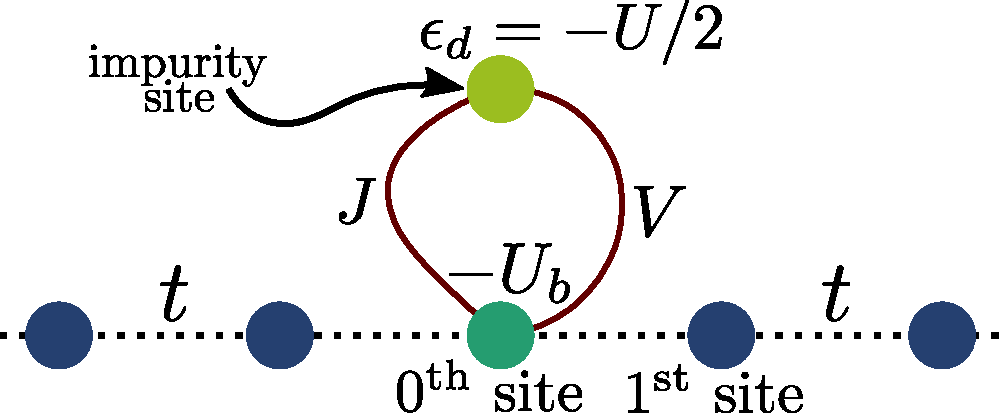
\includegraphics[width=0.95\textwidth]{figures/gen_siam.pdf}
\end{minipage}

\footcite{Schrieffer_Wolff,anderson_impurity_1961}

\end{frame}

\section{The Unitary Renormalization Group Method}
\label{method}
\begin{frame}[noframenumbering]{The Unitary Renormalization Group Method}
\footcite{anirbanurg1,anirbanurg2}

\only<1-3>{
\head{The General Idea}
\begin{minipage}{0.8\textwidth}
\begin{itemize}[<+->]
	\item Apply unitary many-body transformations to the Hamiltonian\\[10pt]
	\item Successively decouple high energy states\\[10pt]
	\item Obtain sequence of Hamiltonians and hence scaling equations
\end{itemize}
\end{minipage}
\begin{minipage}{0.15\textwidth}
\begin{figure}
	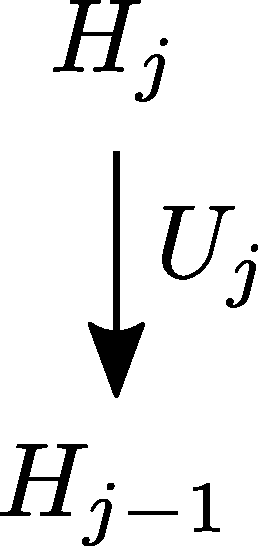
\includegraphics[width=0.7\textwidth]{figures/urg_schematic.pdf}
\end{figure}
\end{minipage}
}

\only<4>{
\head{Select a UV-IR Scheme}
\vspace*{\fill}

\begin{minipage}{0.5\textwidth}
\centering
\focus{UV shell}
\begin{gather*}
	\vec k_N ~~ \left(\text{zeroth RG step}\right)\\
\vdots\\ 
\vec k_j ~ ~ \left(j^\text{th} \text{ RG step}\right) \\
\vdots\\
\vec k_1 ~ ~ \left(\text{Fermi surface}\right)
\end{gather*}
\focus{IR shell}
\end{minipage}
\hspace*{\fill}
\begin{minipage}{0.4\textwidth}
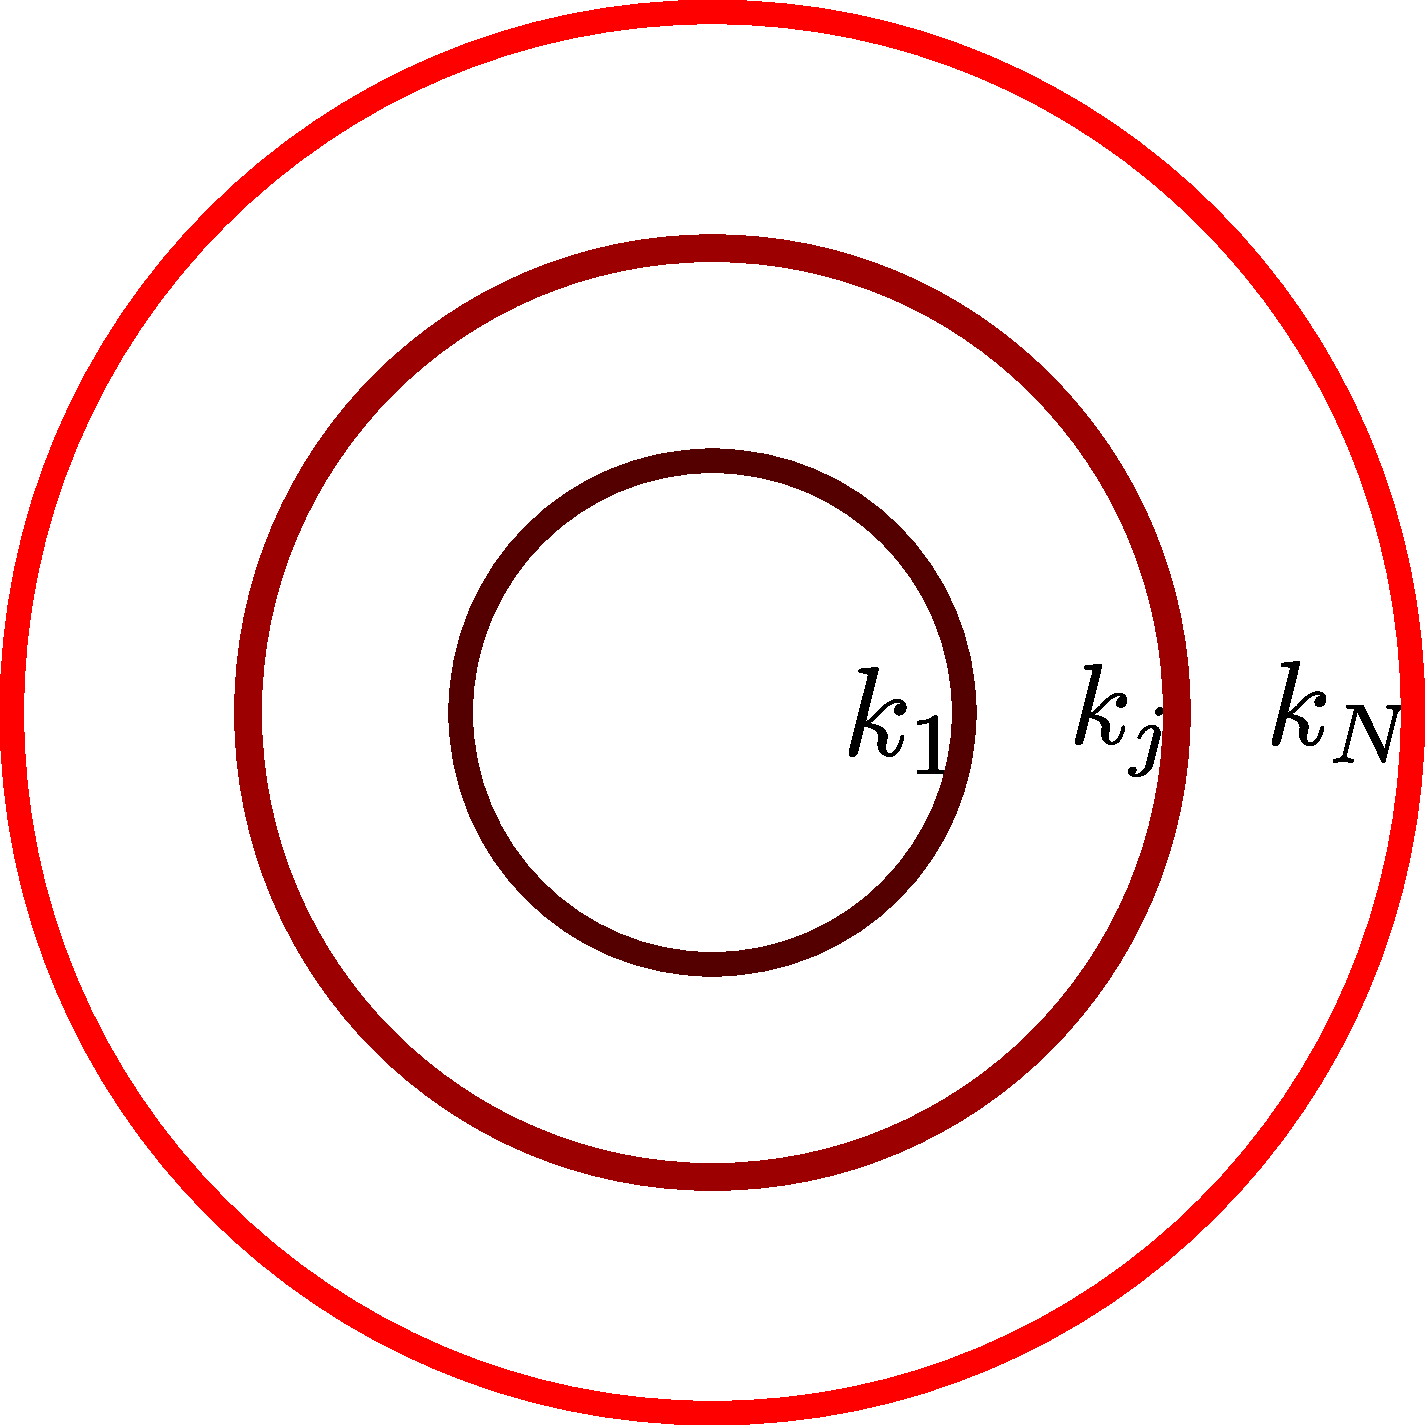
\includegraphics[width=0.9\textwidth]{figures/uv_ir_scheme.pdf}
\end{minipage}
\vspace*{\fill}
}

\only<5>{
\vspace*{-20pt}
\head{Write Hamiltonian in the basis of \(\vec k_j\)}
\vspace*{\fill}

\begin{minipage}{0.4\textwidth}
	\vspace*{-30pt}
	\[H_{(j)} = H_1 \hat n_j + H_0 \left(1 - \hat n_j\right) + c^\dagger_j T + T^\dagger c_j\]
\[
 {2^{j-1} \text{-dim.}} \longrightarrow \begin{cases}
	H_1, H_0 \longrightarrow \text{diagonal parts}\\
T \longrightarrow \text{off-diagonal part}
\end{cases}
\]
\[ (j) : j^\text{th} \text{ RG step}\]
\end{minipage}
\hspace*{\fill}
\begin{minipage}{0.5\textwidth}
\begin{figure}
	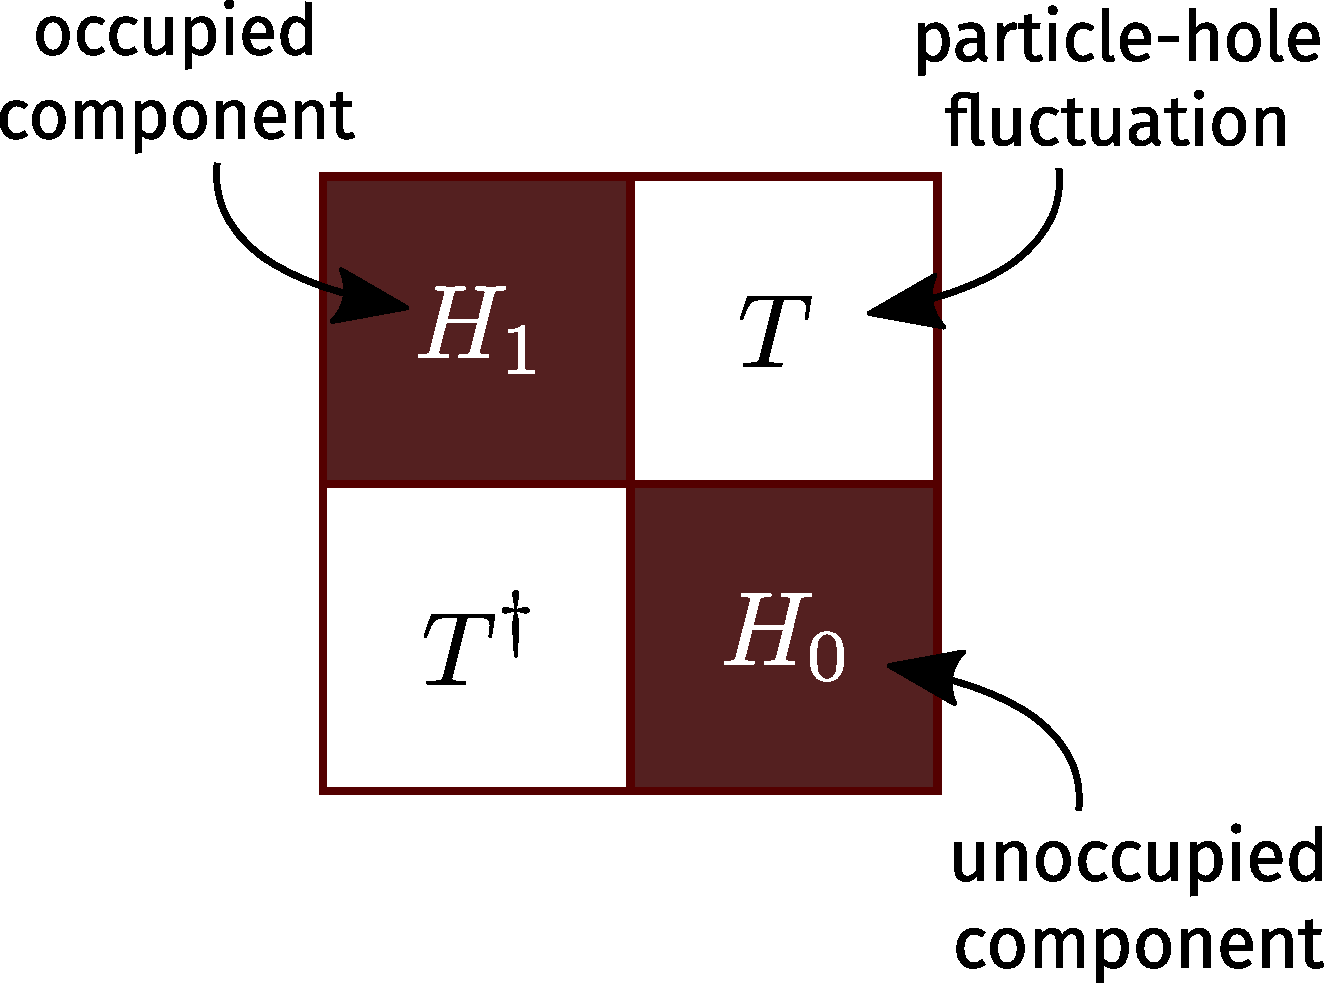
\includegraphics[width=0.9\textwidth]{figures/urg_ham.pdf}
\end{figure}
\end{minipage}
}
\only<6>{
\vspace*{-10pt}
\head{Rotate Hamiltonian and kill off-diagonal blocks}

\vspace*{\fill}

\begin{minipage}{0.45\textwidth}
\centering
\[H_{(j-1)} = U_{(j)} H_{(j)} U_{(j)}^\dagger\]
\[U_{(j)} = \frac{1}{\sqrt 2}\left(1 - \eta_{(j)} + \eta_{(j)}^\dagger\right), ~ ~ \left\{\eta_{(j)}, \eta^\dagger_{(j)}\right\} = 1 \]
\[ \eta^\dagger_{(j)} = \frac{1}{\hat \omega_{(j)} - H_D}c^\dagger_j T \Bigg \} \rightarrow {\text{many-particle}\atop{\text{rotation}}}\]
\[\hat \omega_{(j)} = \left(H_{1} + H_{0}\right)_{(j-1)} + \Delta T_{(j)}\]
\[\text{\focus{\Big(quantum fluctuation operator\Big)}}\]
\vspace*{\fill}
\end{minipage}
\hspace*{\fill}
\begin{minipage}{0.5\textwidth}
\begin{figure}
	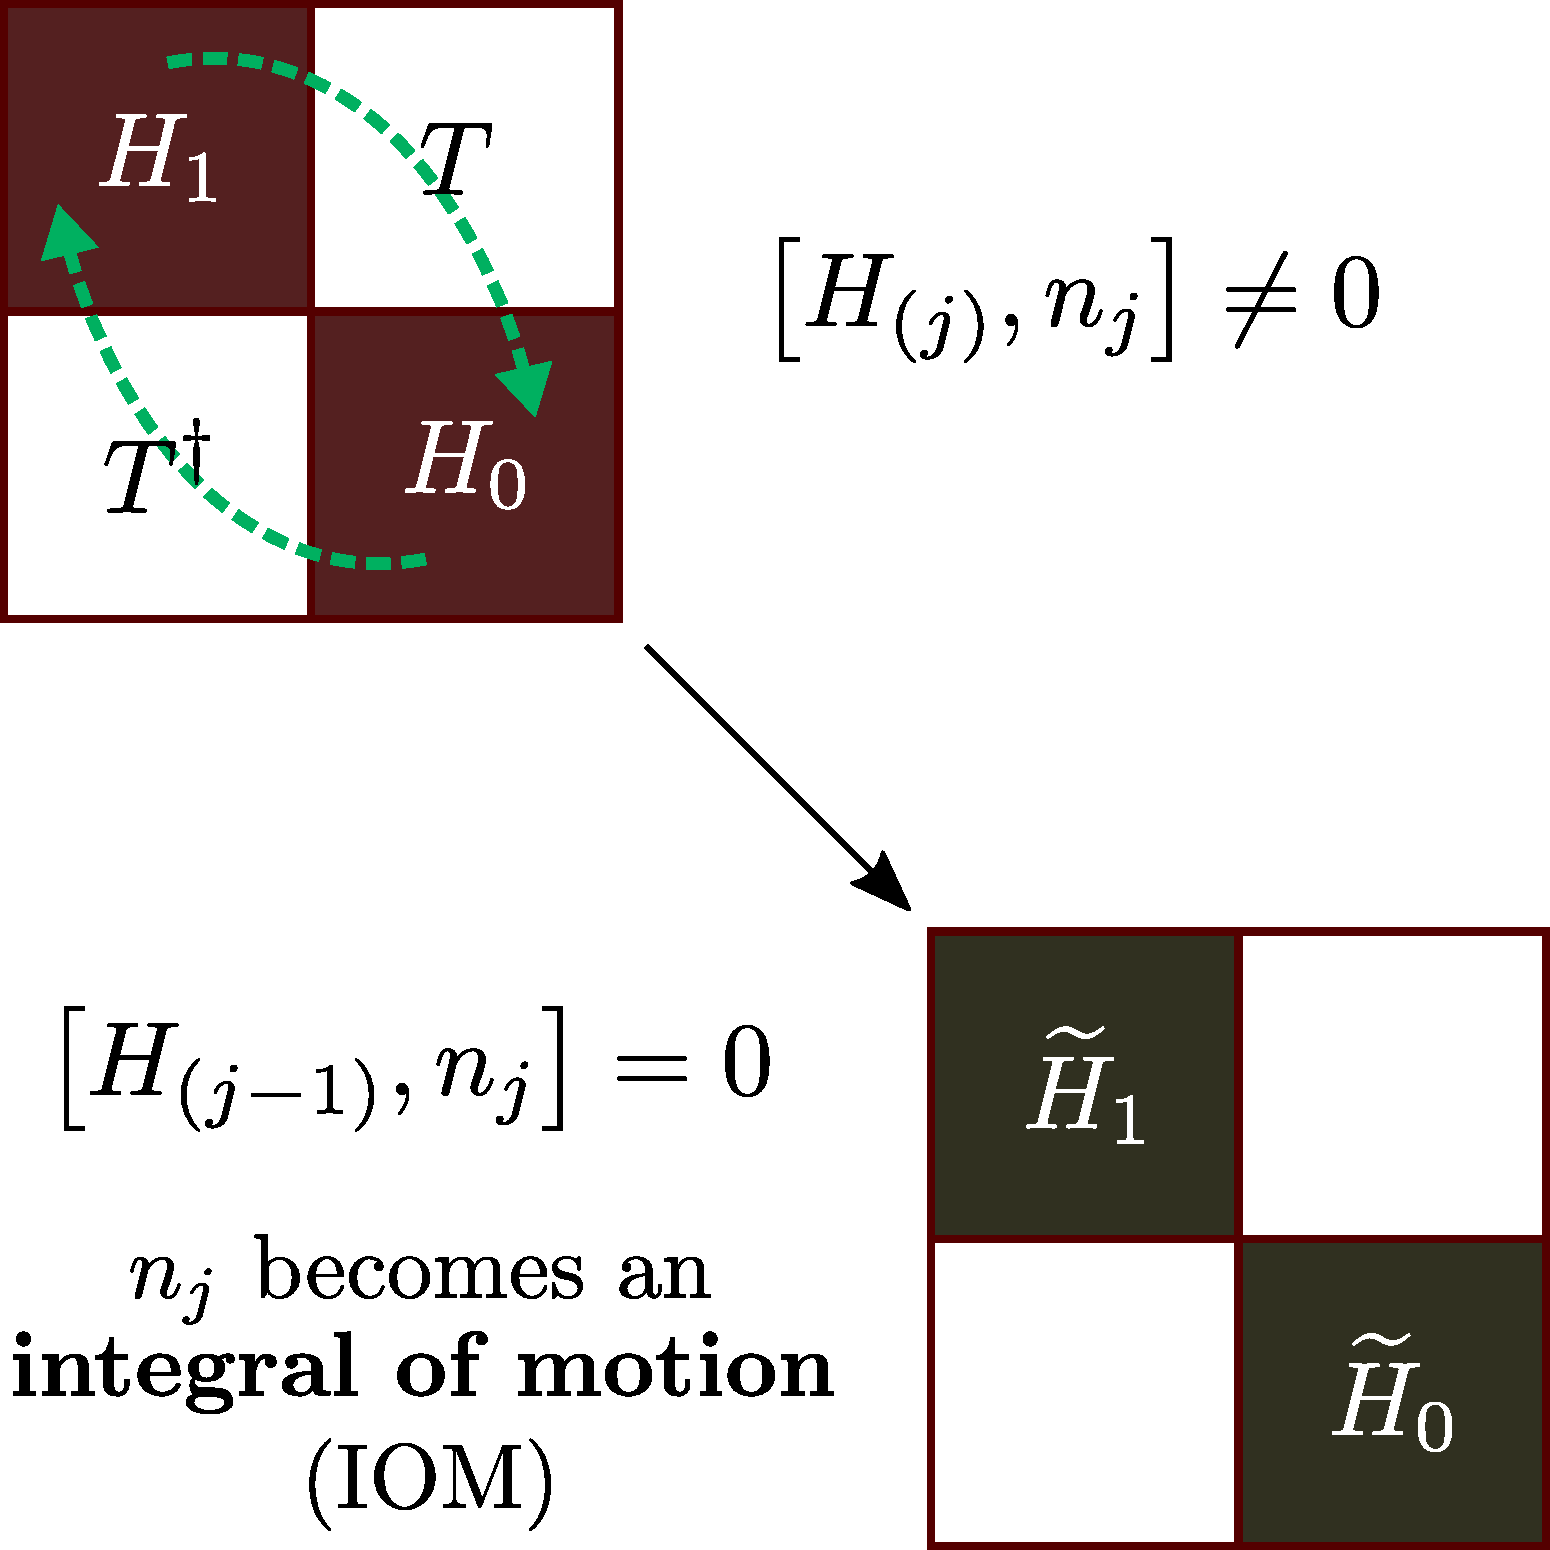
\includegraphics[width=0.8\textwidth]{figures/urg_rot.pdf}
\end{figure}
\end{minipage}
}

\only<7>{

\head{Repeat with renormalised Hamiltonian}

\begin{minipage}{0.53\textwidth}
	\[H_{(j-1)} = \widetilde H_1 \hat n_j + \widetilde H_0 \left(1 - \hat n_j\right)\]
	\[\widetilde H_1 = H_1 \hat n_{j-1} + H_0 \left(1 - \hat n_{j-1}\right) + c^\dagger_{j-1} T + T^\dagger c_{j-1}\]
\vspace*{\fill}
\end{minipage}
\hspace*{\fill}
\begin{minipage}{0.45\textwidth}
\begin{figure}
	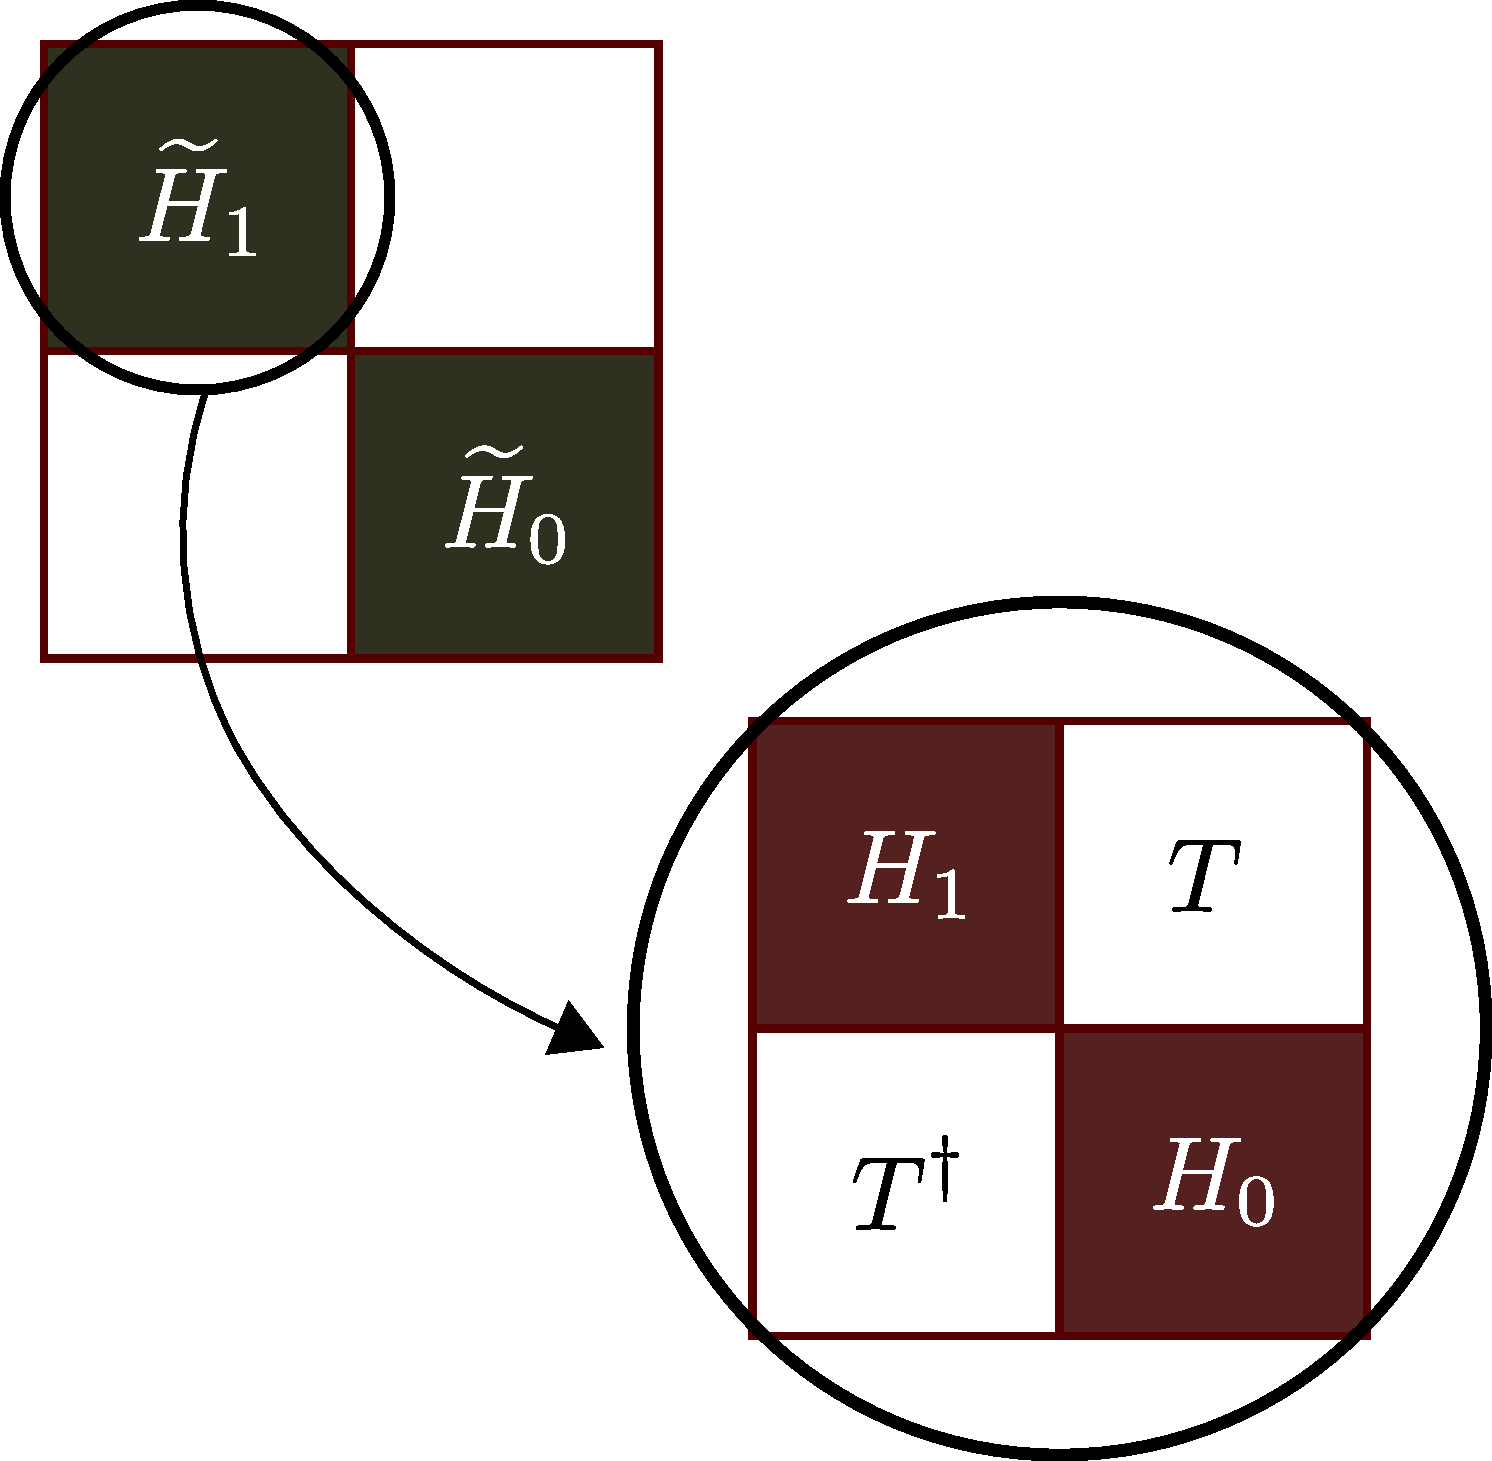
\includegraphics[width=\textwidth]{figures/urg_next.pdf}
\end{figure}
\end{minipage}
}

\only<8>{
\vspace*{-30pt}
\head{RG Equations and Denominator Fixed Point}

\vspace*{40pt}
\begin{minipage}{0.4\textwidth}
	\centering
\[ \Delta H_{(j)} = \left(\hat n_j - \frac{1}{2}\right) \left\{c^\dagger_j T, \eta_{(j)}\right\} \]
\[\eta^\dagger_{(j)} = \frac{1}{\hat \omega_{(j)} - H_D}c^\dagger_j T\] 
\[\text{{Fixed point:}}~ ~ ~\hat \omega_{(j^*)} - \left(H_D\right)^* = 0\]
\focus{eigenvalue of \(\hat \omega\) coincides with that of \(H\)}
\end{minipage}
\hspace*{\fill}
\begin{minipage}{0.58\textwidth}
	\centering
	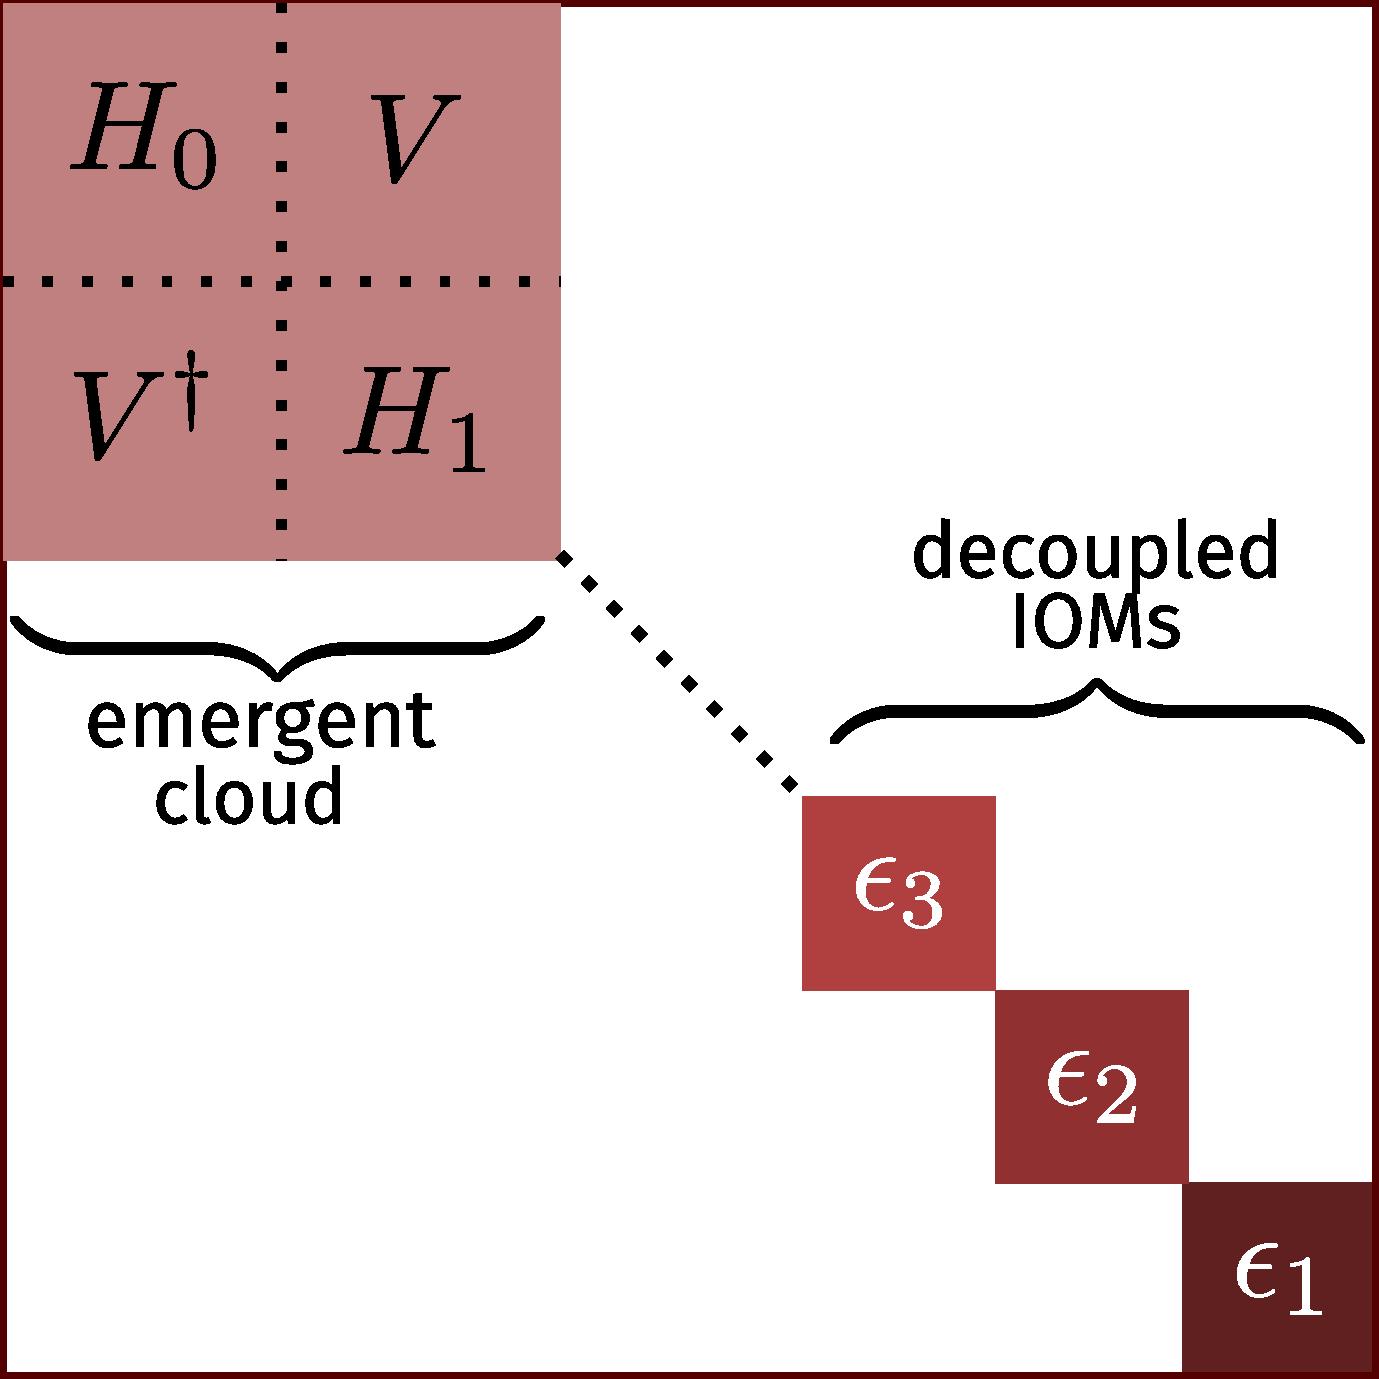
\includegraphics[width=0.65\textwidth]{figures/urg_ham_full.pdf}
\end{minipage}
\vspace*{\fill}
}
\end{frame}

\begin{frame}[noframenumbering]{The Unitary Renormalization Group Method}
\head{Novel Features of the Method}
% \hspace*{-20pt}
\begin{minipage}{0.65\textwidth}
\begin{itemize}[<+->]
	\item \focus{Quantum fluctuation scale} \(\hat \omega\)	that tracks all orders of renormalisation\\[10pt]
	\item Finite-valued fixed points for finite systems - leads to \focus{emergent degrees of freedom}\\[10pt]
	\item \focus{Spectrum-preserving} unitary transformations - partition function does not change\\[10pt]
	\item Tractable low-energy effective Hamiltonians - allows \focus{renormalised perturbation theory} around them 
\end{itemize}
\end{minipage}
\hspace*{\fill}
\begin{minipage}{0.3\textwidth}
\begin{flushleft}
	\(H_{(j-1)} = U_{(j)} H_{(j)} U_{(j)}^\dagger\)\\[15pt]
	\(U_{(j)} = \frac{1}{\sqrt 2}\left(1 - \eta_{(j)} + \eta_{(j)}^\dagger\right) \)\\[15pt]
	\( \eta^\dagger_{(j)} = \frac{1}{\hat \omega_{(j)} - H_D}c^\dagger_j T\)\\[15pt]
	\( \Delta H_{(j)} = \left(\hat n_j - \frac{1}{2}\right) \left\{c^\dagger_j T, \eta_{(j)}\right\} \)
\end{flushleft}
\end{minipage}
\end{frame}
\section{URG Analysis: \(U_b=0\)}
\label{urg-1}
\begin{frame}[noframenumbering]{\(U_b = 0:\) Flow towards strong-coupling}
\centering
% \vspace*{-10pt}
{\(\mathbf{U > 0, J > 0}\)}

\vspace*{10pt}

\only<+>{
\centering

{\large \(\Delta V = \frac{3n_j VJ}{8}\left(\frac{1}{|d_2|} + \frac{1}{|d_1|}\right) > 0\), ~ ~ \(\Delta J = \frac{n_j J^2}{|d_2|} > 0\)}

{\large \(d_0 = \omega - \frac{D}{2} - \frac{U}{2} + \frac{K}{4}, \quad d_1 = \omega - \frac{D}{2} + \frac{U}{2} + \frac{J}{4}\), ~ ~
\(d_2 = \omega - \frac{D}{2} + \frac{J}{4}\)}

\hspace*{-50pt}
\vspace*{-20pt}

	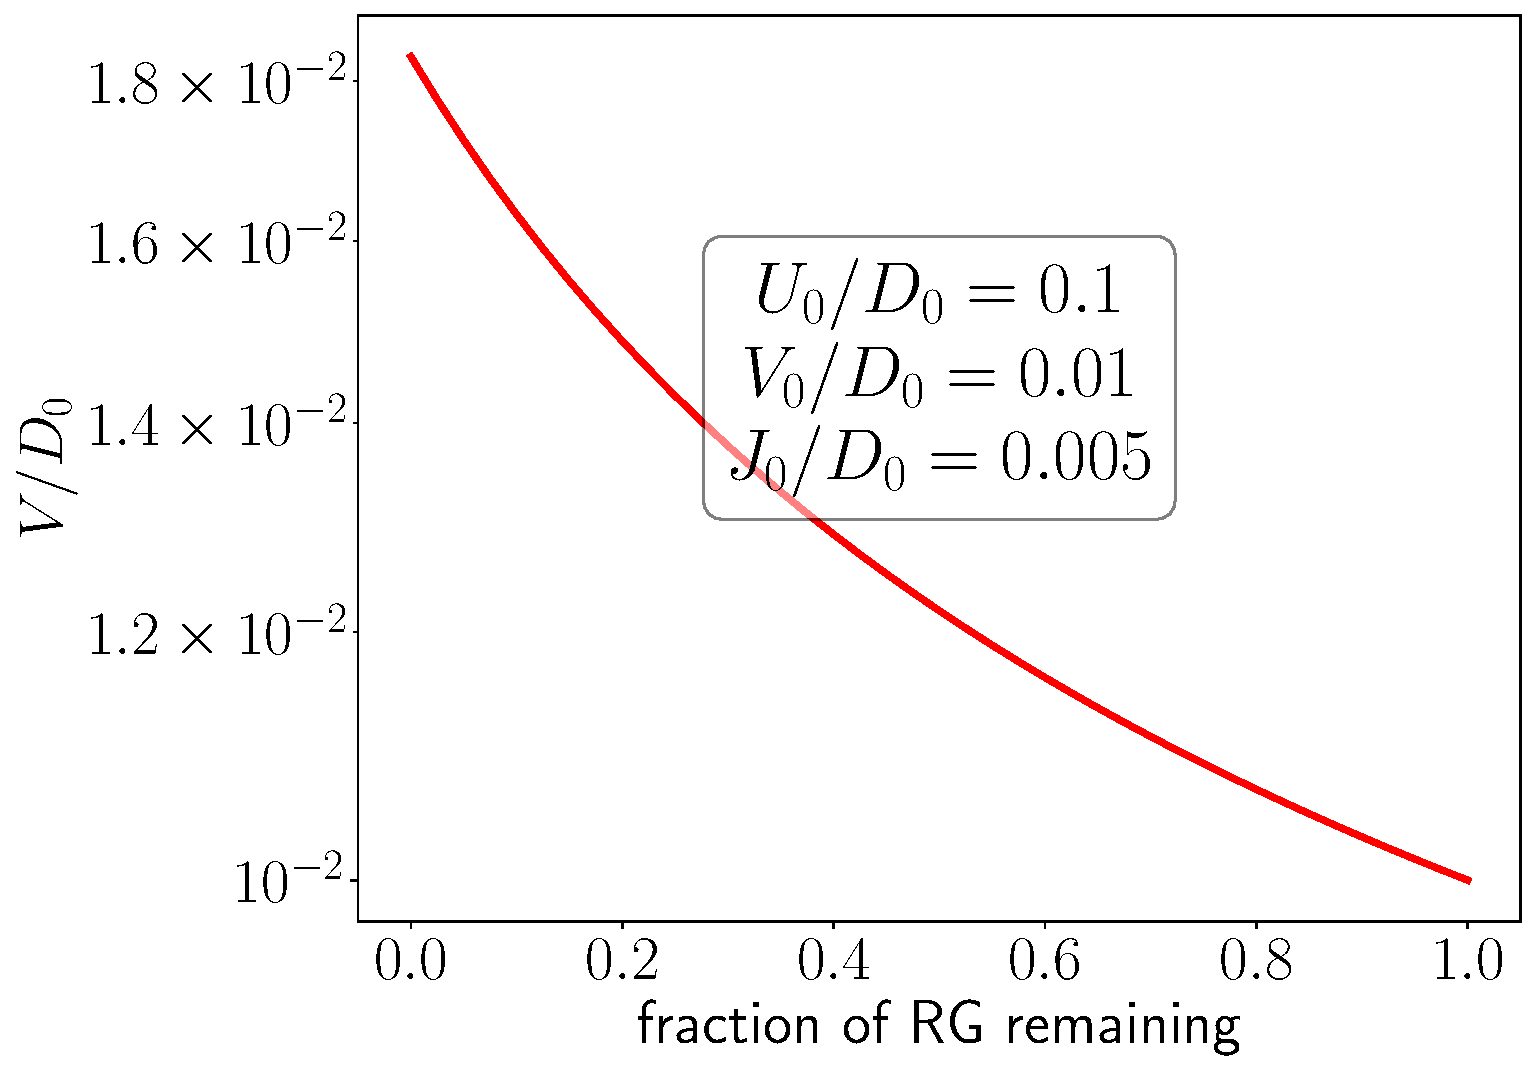
\includegraphics[width=0.49\textwidth]{figures/U_irr,U>0,V.pdf}
	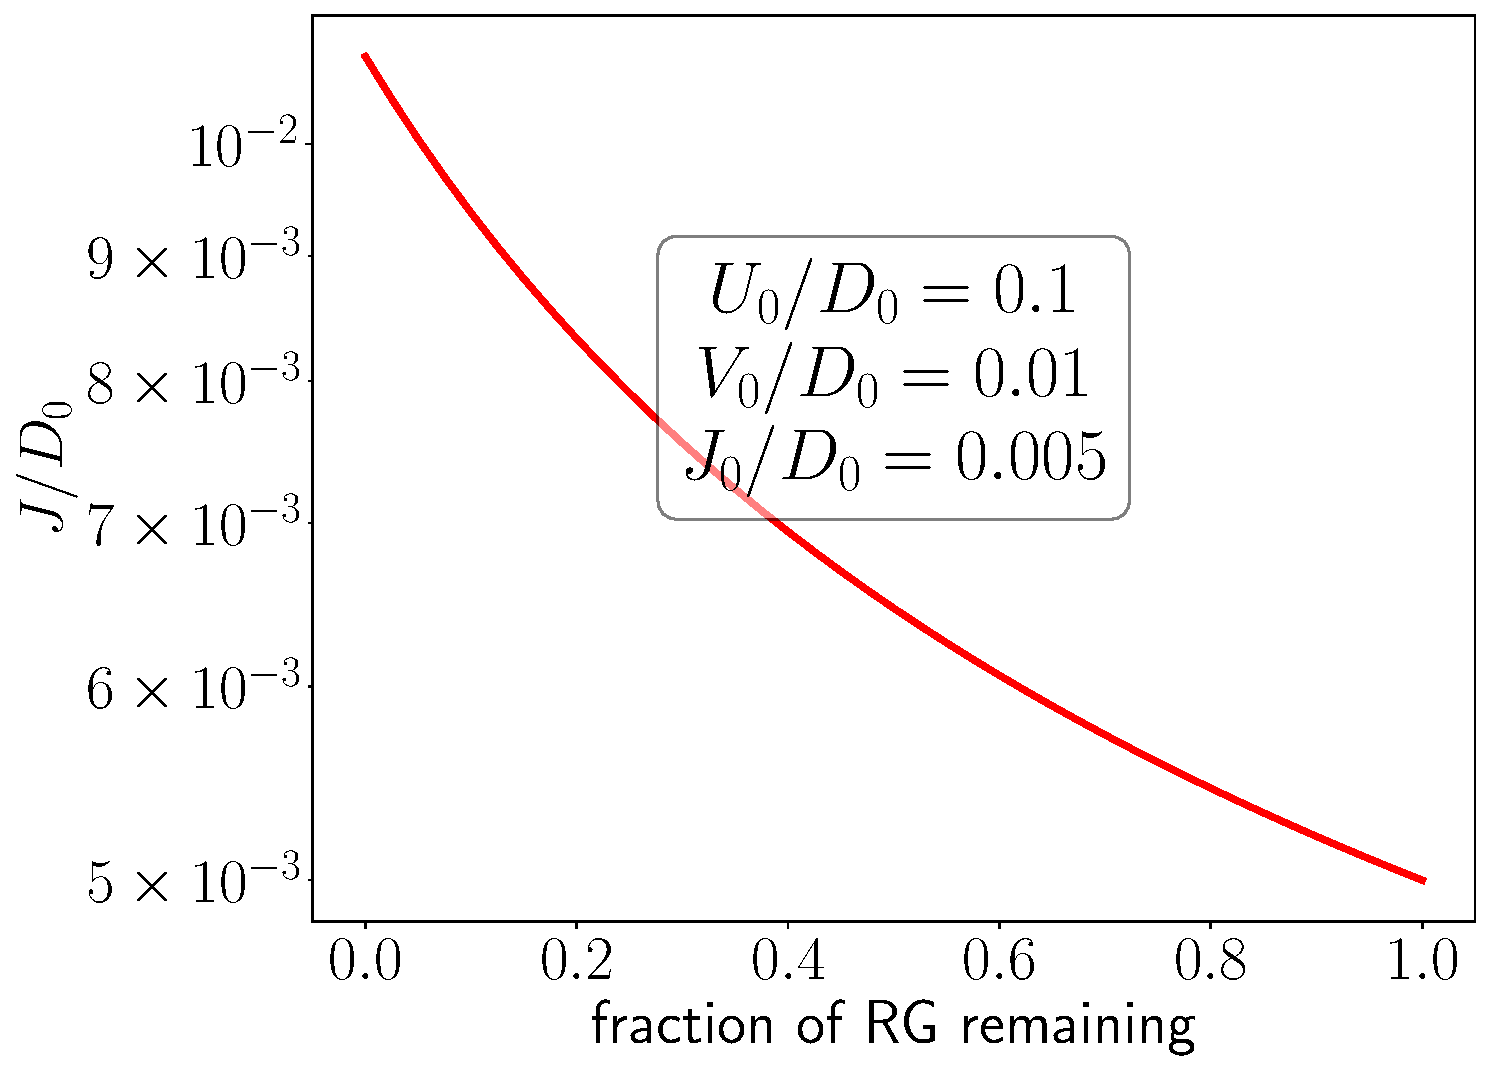
\includegraphics[width=0.49\textwidth]{figures/U_irr,U>0,J.pdf}
}
\only<+>{
{\large \(\Delta U = 4V^2 n_j\left(\frac{1}{d_1} - \frac{1}{d_0}\right) - n_j\frac{J^2}{d_2}\)}

% \vspace*{-10pt}

\begin{minipage}{0.49\textwidth}
\centering
{\large\( V > J\)}

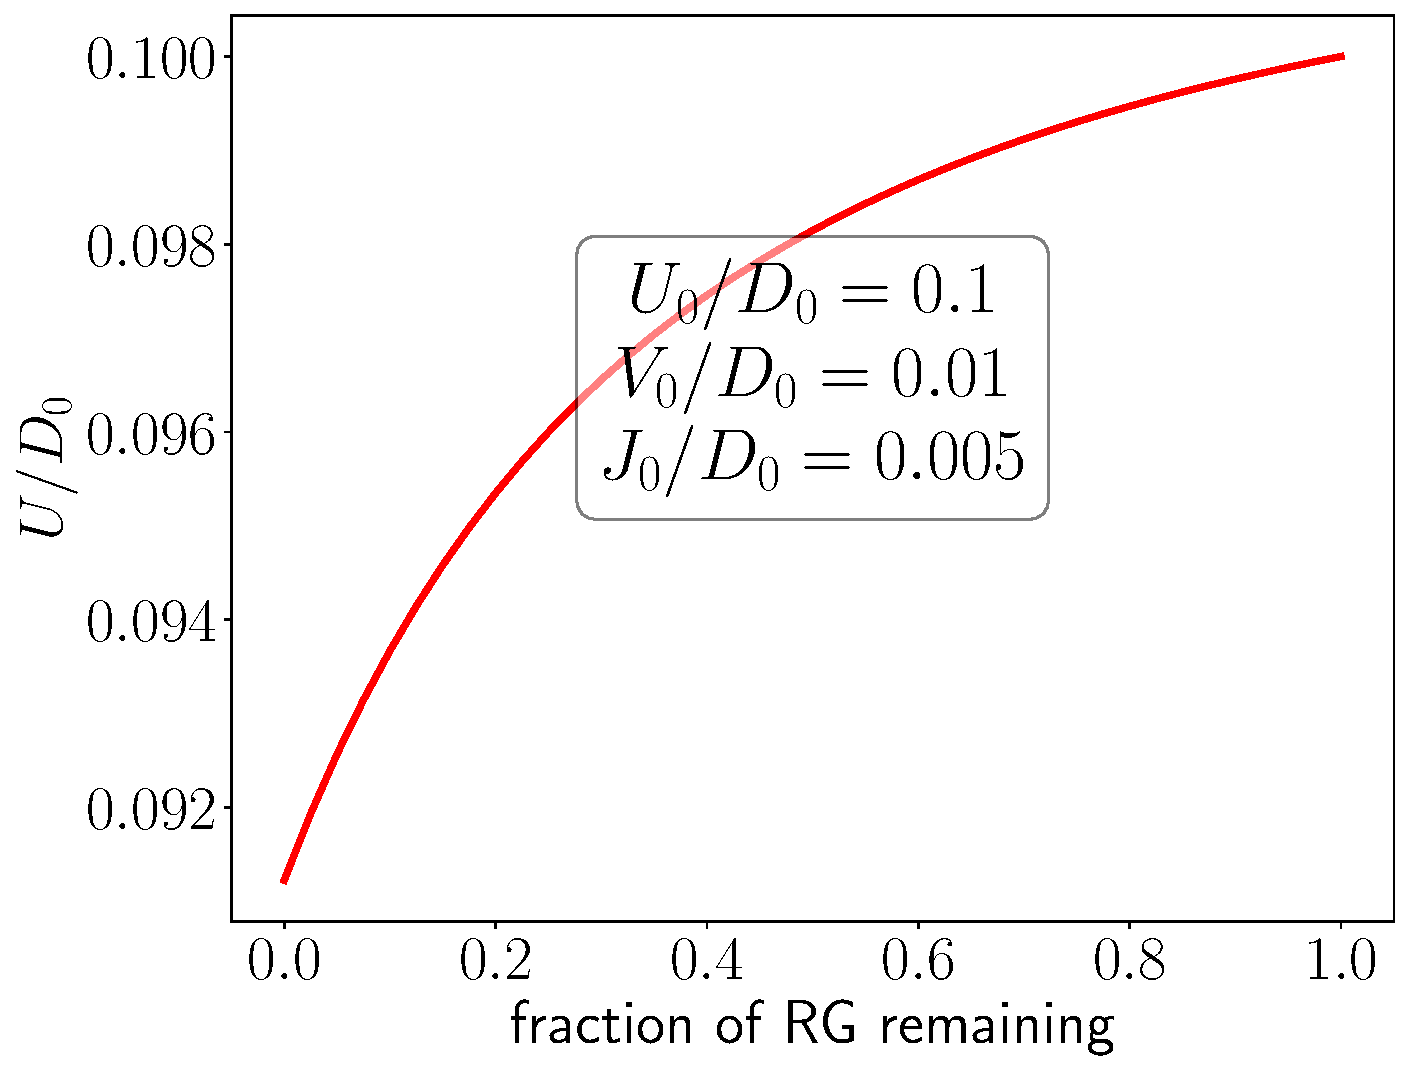
\includegraphics[width=\textwidth]{figures/U_irr,U>0,U.pdf}
\end{minipage}
\begin{minipage}{0.49\textwidth}
\centering
{\large\( V < J\)}

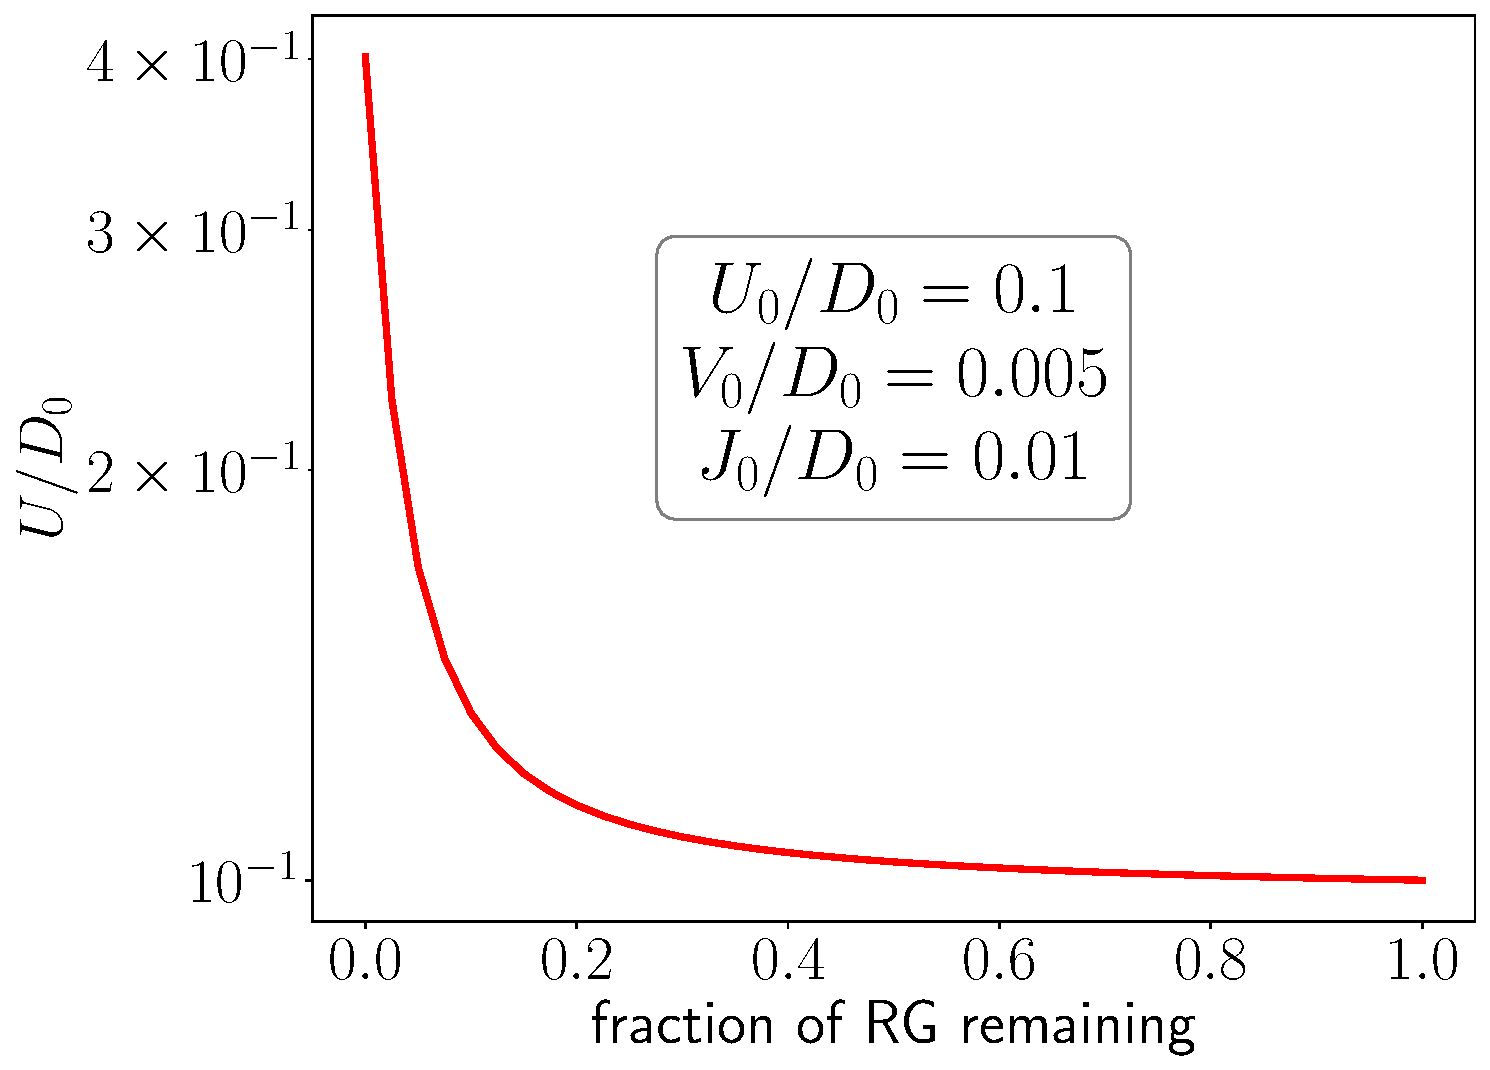
\includegraphics[width=\textwidth]{figures/U_rel,U>0,U.pdf}
\end{minipage}
}

\end{frame}

\begin{frame}[noframenumbering]{\(U > 0\) Fixed point Hamiltonian}
\begin{minipage}{0.48\textwidth}
	\[H^* = \sum_{k < k^*,\sigma}\epsilon_{k}\hat{n}_{k\sigma} ~ + \frac{U^*}{2}\left(\hat n_{d \uparrow} - \hat n_{d \downarrow}\right)^2 ~ + J^* \vec{S}_d\cdot \vec{s}_<\]
	\[+ ~ V^* \sum_{k < k^*,\sigma}\left(c^\dagger_{d\sigma}c_{k\sigma} + \text{h.c.}\right)\]

	\vspace*{20pt}
	\[\vec{s}_< = \frac{1}{2}\sum_{k,k^\prime < k^*}c^{\dagger}_{k\alpha}\vec{\sigma}_{\alpha\beta}c_{k^\prime,\beta}\]
\end{minipage}
\begin{minipage}{0.5\textwidth}
	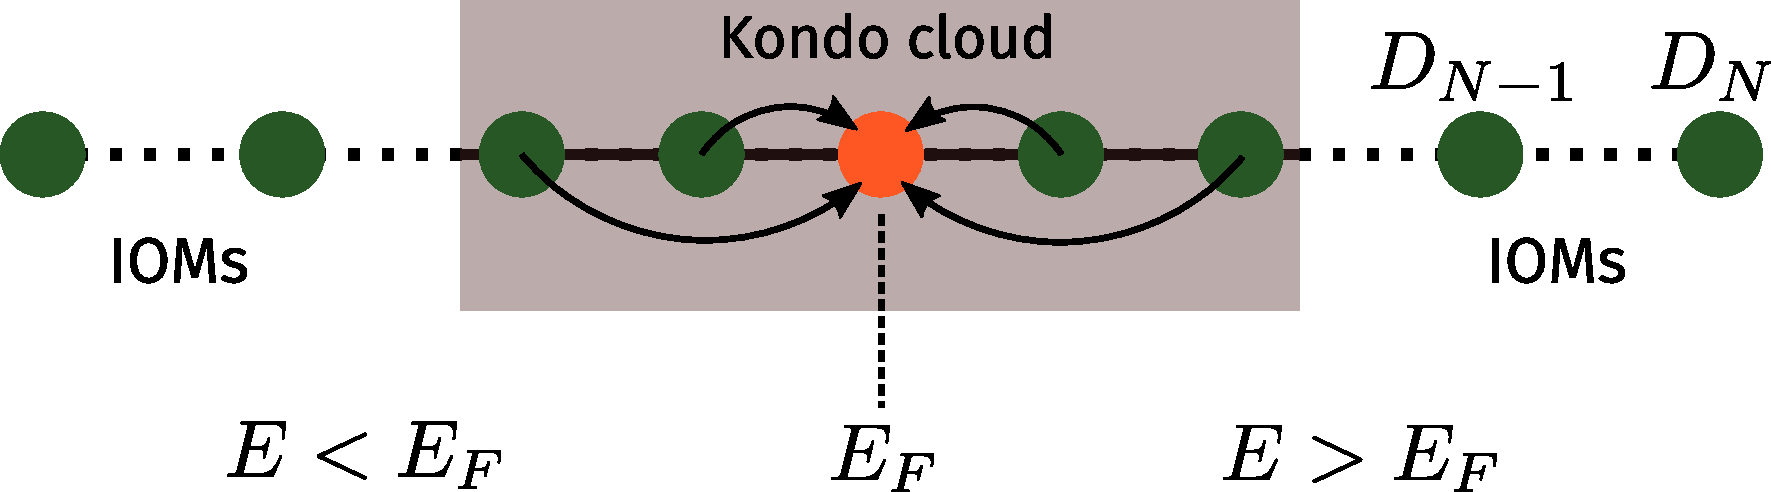
\includegraphics[width=\textwidth]{figures/kondo_fp_1D.pdf}
\end{minipage}
\end{frame}

\begin{frame}[noframenumbering]{Impurity Spectral Function}
\centering

\focus{no gap} at arbitrarily large $U$

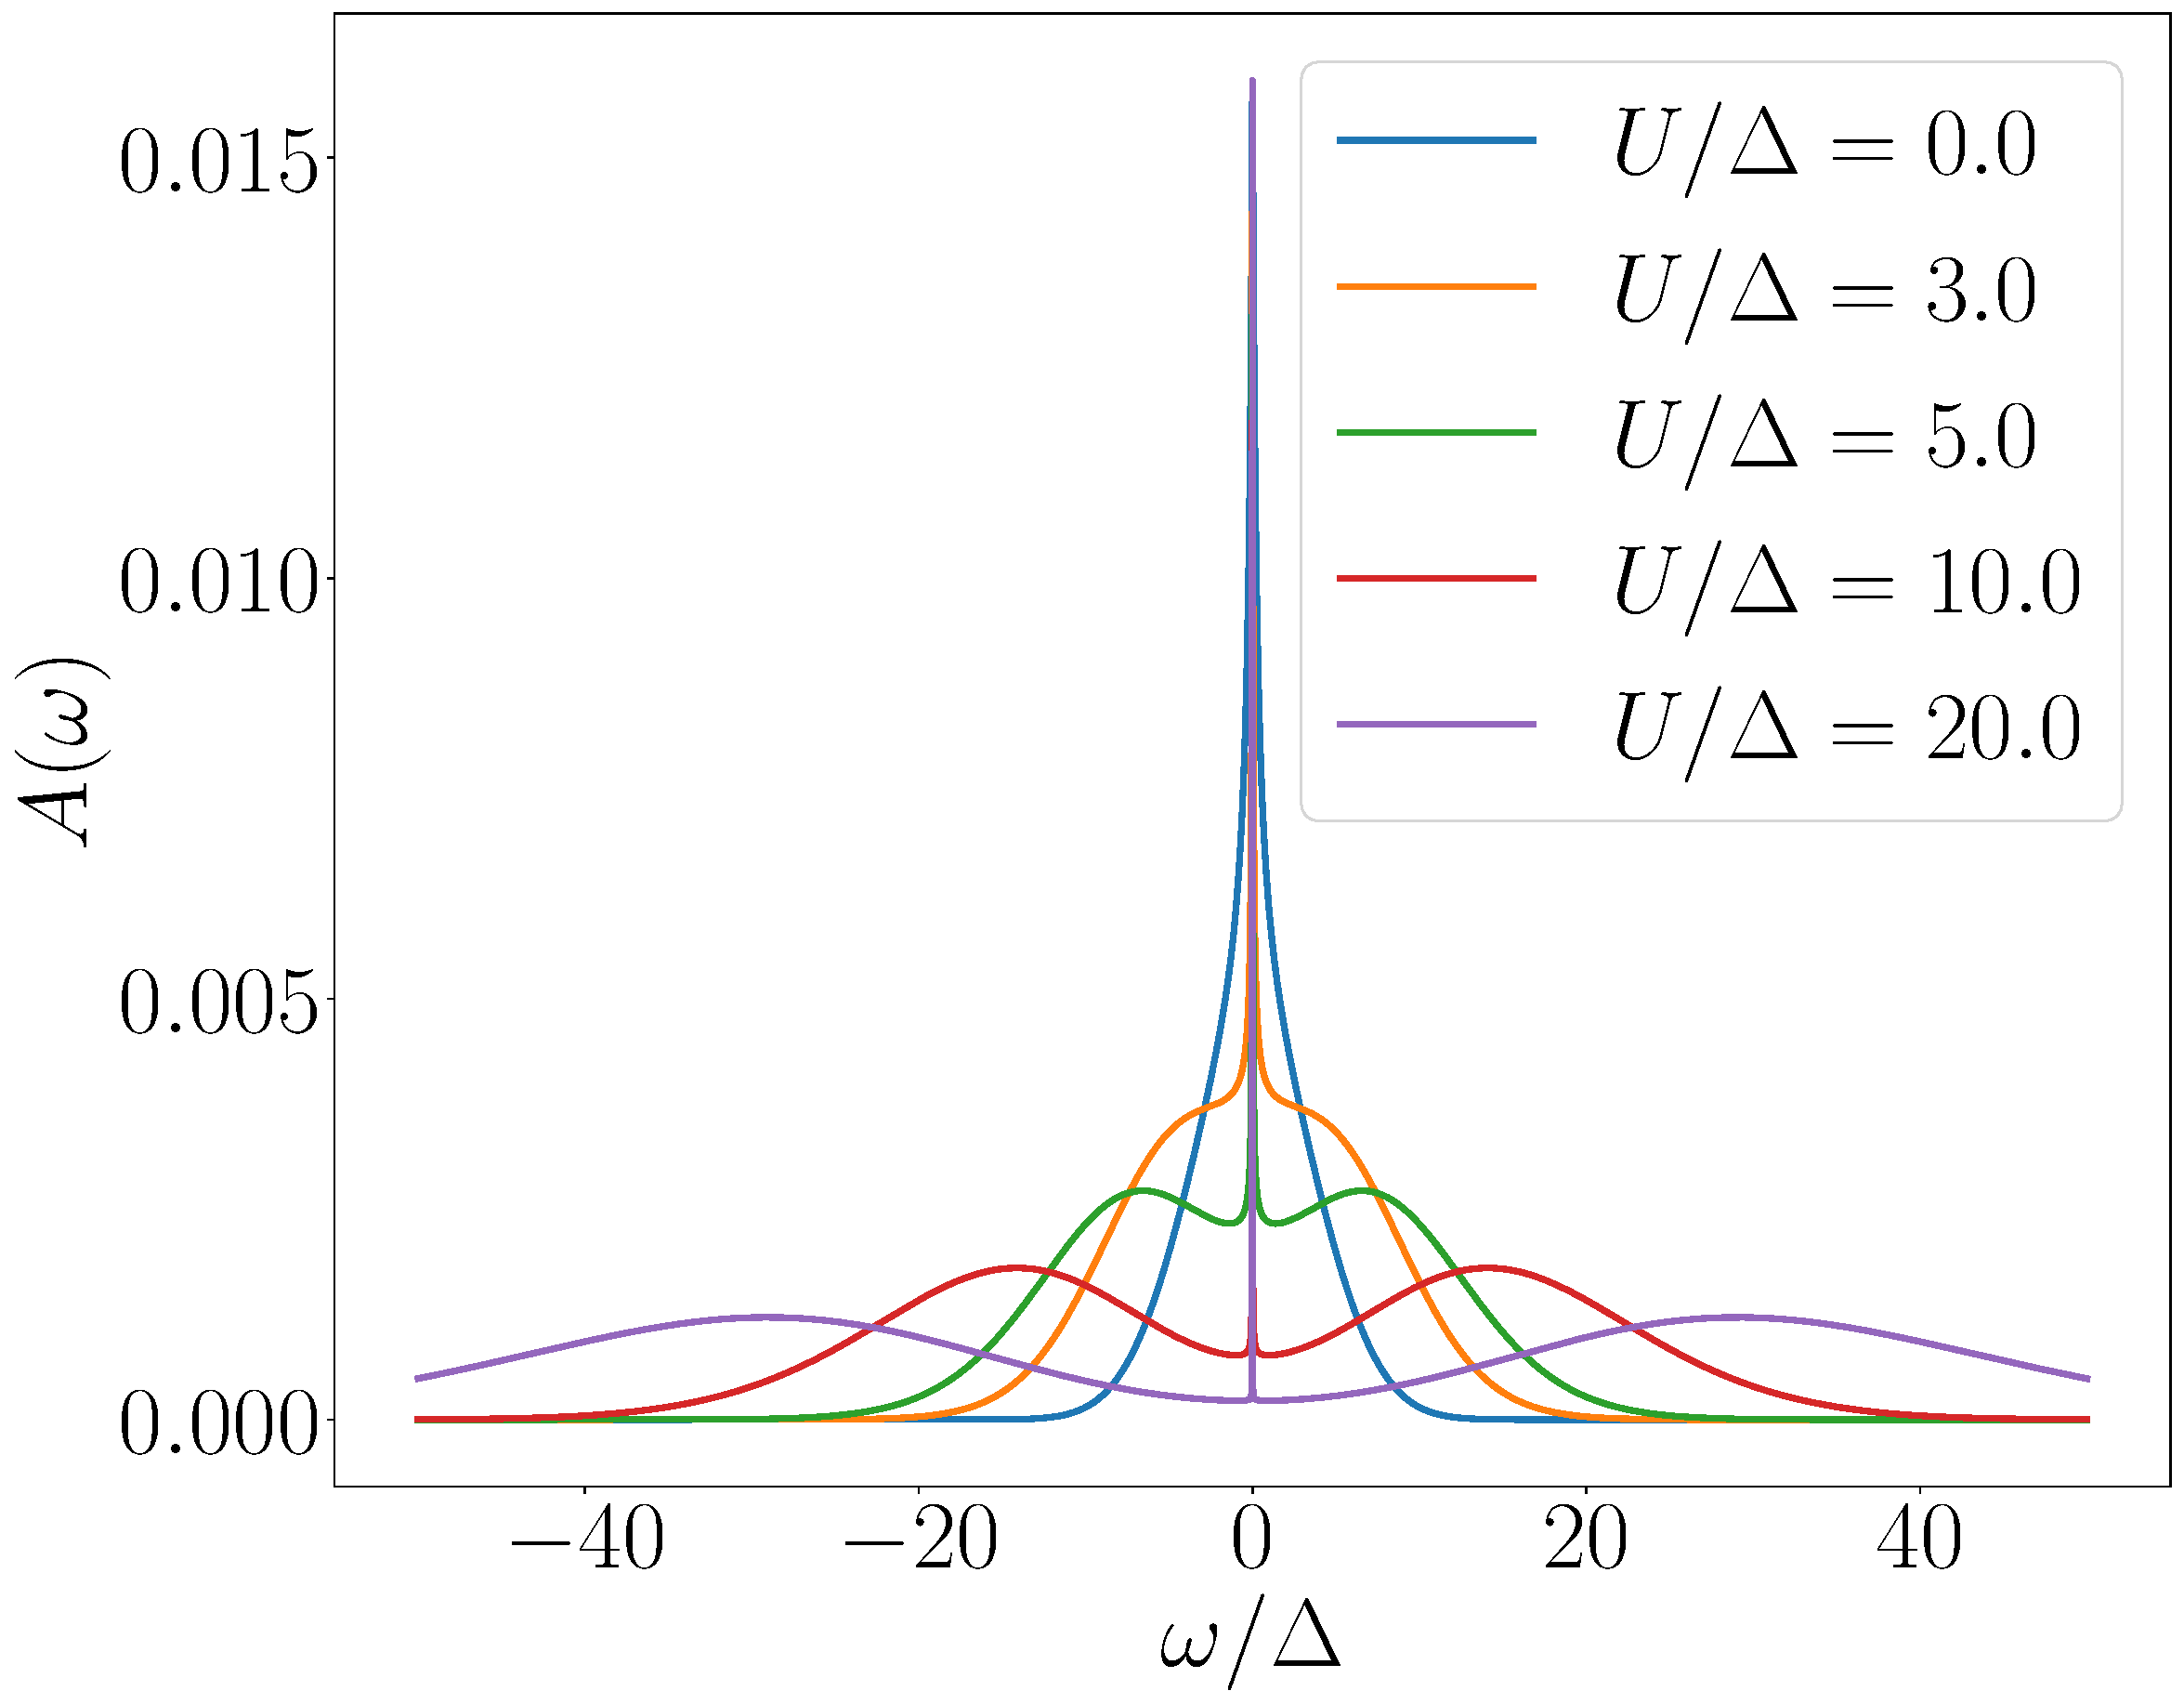
\includegraphics[width=0.6\textwidth]{./figures/gen_siam_spec_func.pdf}

\end{frame}

\section{URG Analysis: \(U_b \neq 0\)}
\label{urg-2}

\begin{frame}[noframenumbering]{\(U > 0\) RG Equations}

\begin{itemize}[<+->]
	\item \(U_b\) is \focus{marginal}: ~ ~ ~\(\Delta U_b = 0\)
	\item Spin-exchange couling \(J\) can now be \focus{driven irrelevant} by \(U_b\): 
	\begin{equation*}
	\Delta J = -\frac{n_j J\left(J + 4U_b\right)}{d_2} \longrightarrow \begin{cases}
	\text{\textcolor{blue}{relevant} when }J+4U_b > 0\\
	\text{\textcolor{red}{irrelevant} when }J+4U_b < 0\\
	\end{cases}
	\end{equation*}
	\item Same can be said for the hybridisation \(V\):
	\begin{equation*}
	\Delta V = -\frac{3n_j V}{8}\left[\left(J + \frac{4U_b}{3}\right) \left(\frac{1}{d_2} + \frac{1}{d_1}\right) + \frac{4U_b}{3}\left(\frac{1}{d_3} + \frac{1}{d_0}\right)\right] \longrightarrow \begin{cases}
	\text{\textcolor{blue}{rel.},}J+4U_b > 0\\
	\text{\textcolor{red}{irrel.},}J+4U_b < 0\\
	\end{cases}
	\end{equation*}
	\item \focus{\(U\) can be relevant if \(J\) decays slower than \(V\)}; needs to be checked numerically
\end{itemize}
\end{frame}

\begin{frame}[noframenumbering]{\(U > 0\) Phase Diagram}
\hspace*{-15pt}
\begin{minipage}{0.5\textwidth}
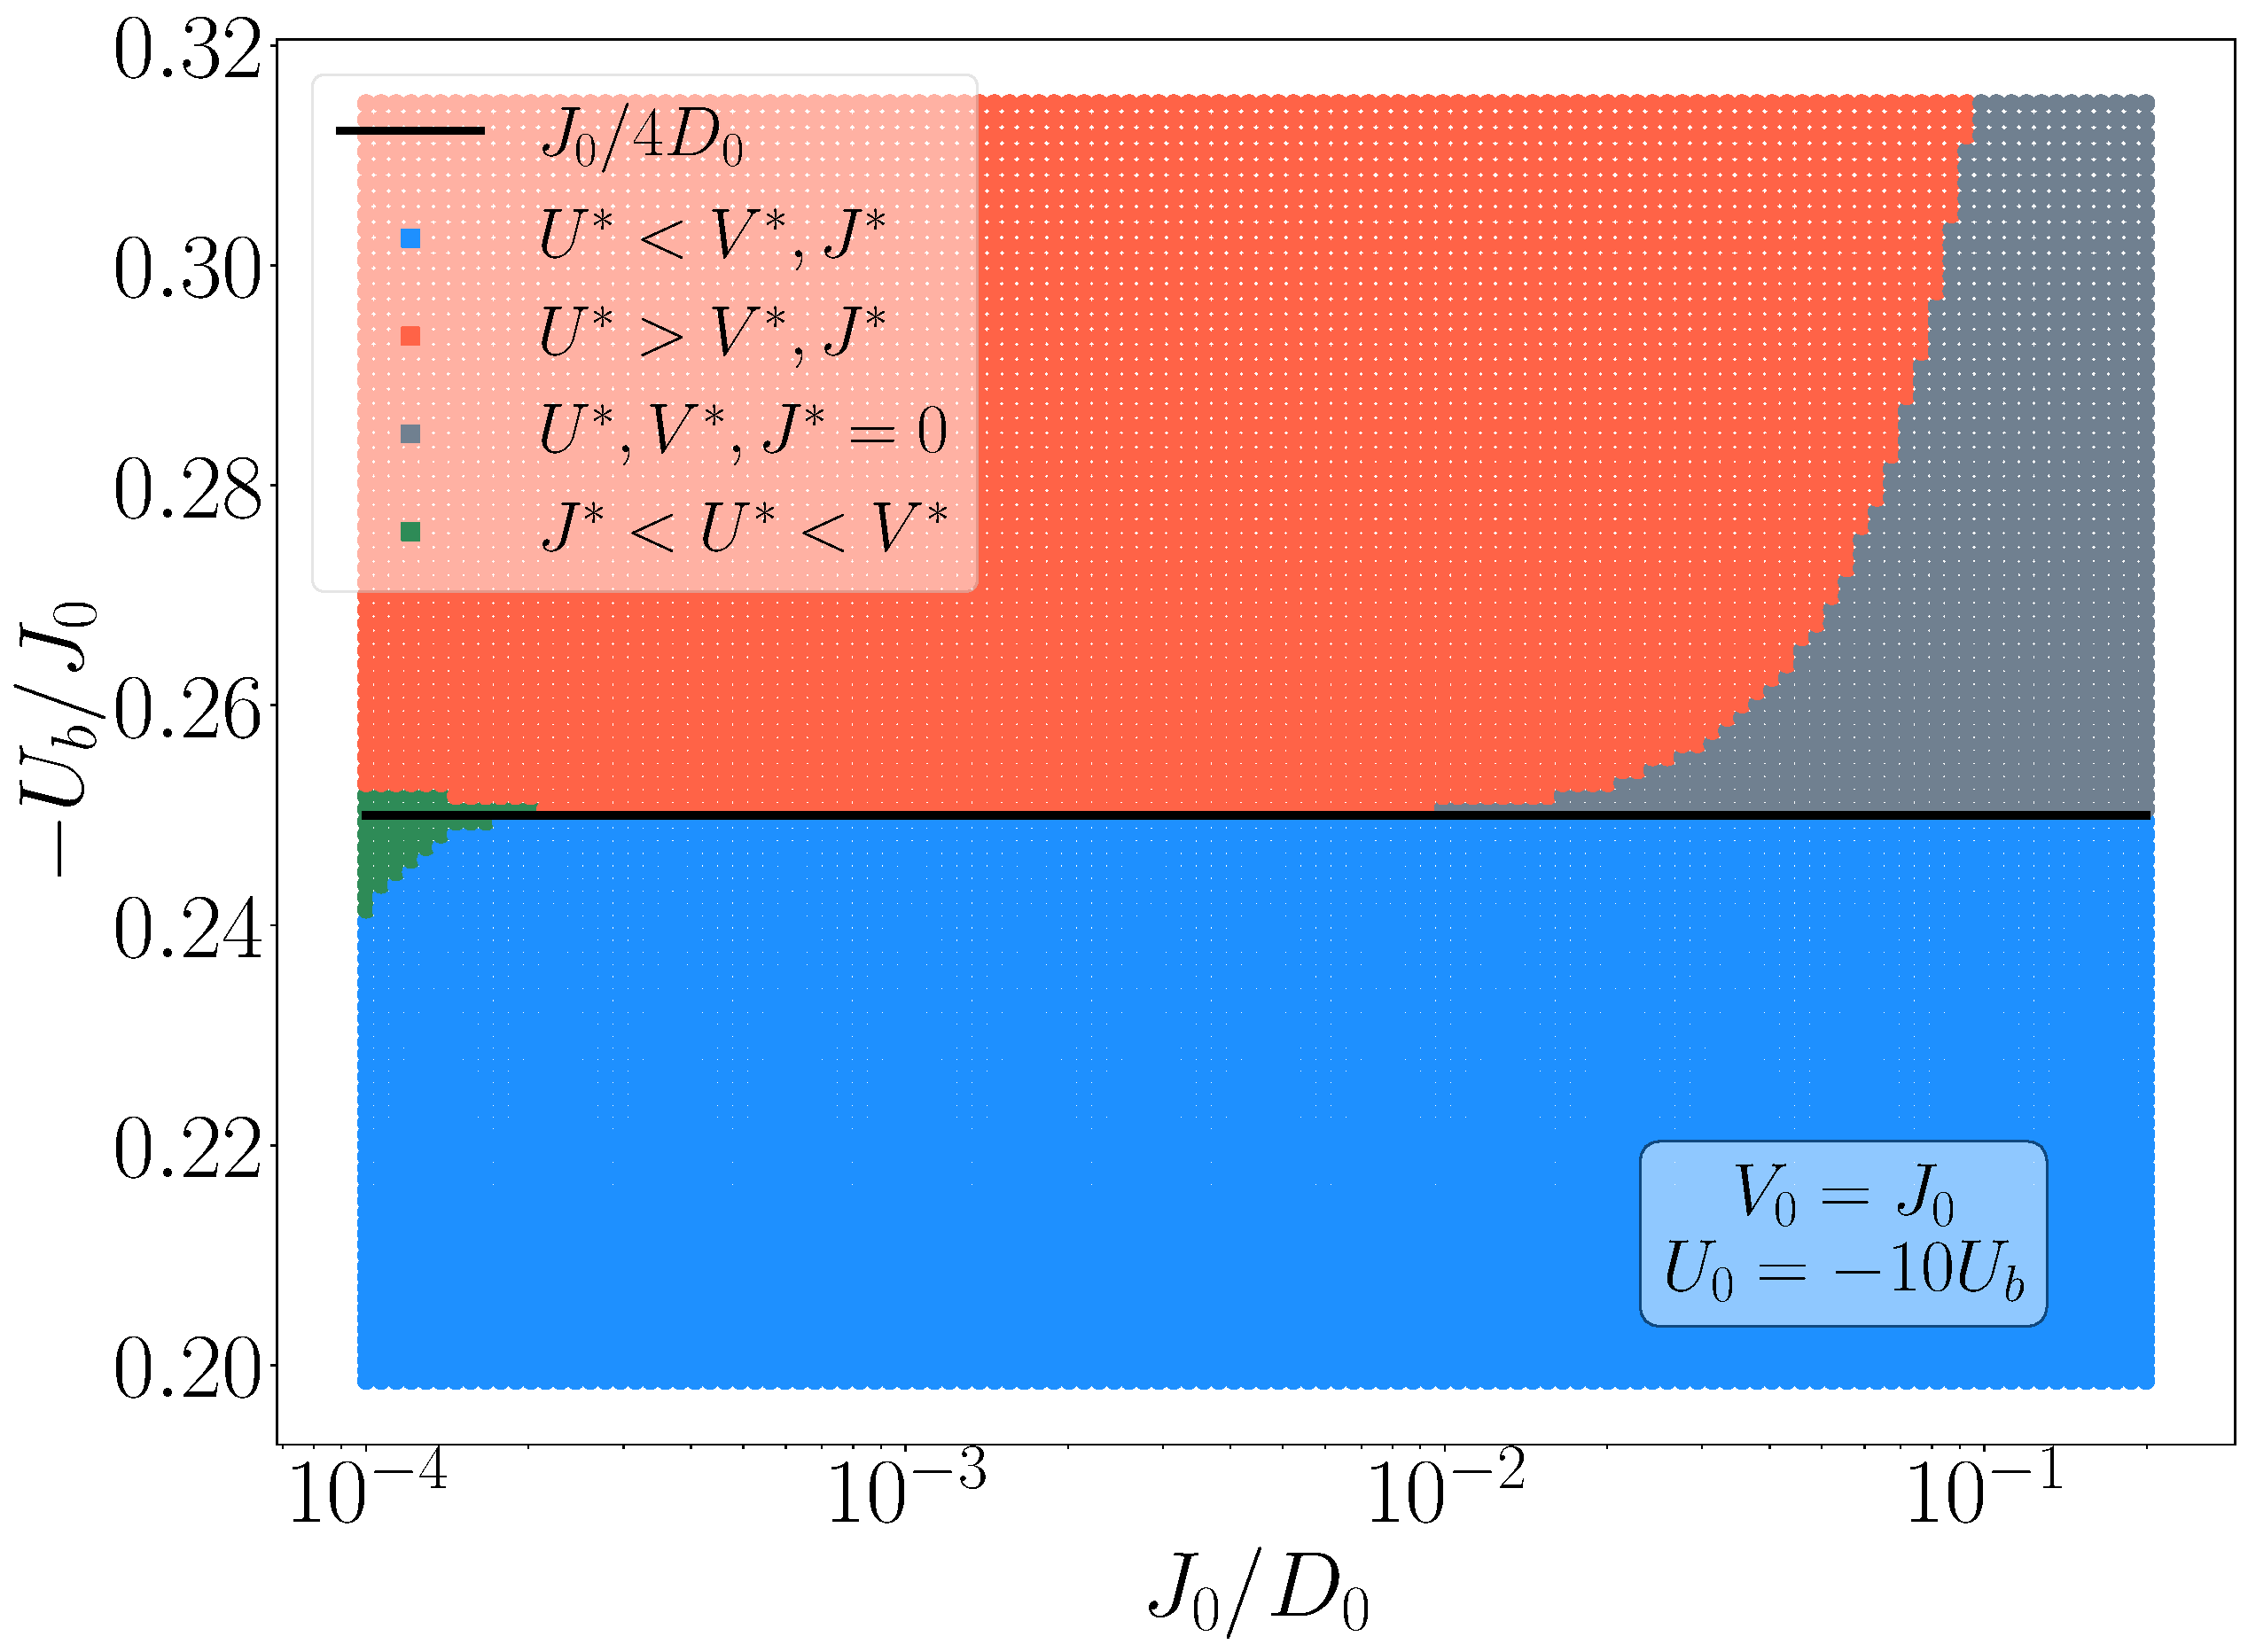
\includegraphics[width=\textwidth]{./figures/phase-map-MIT.pdf}
\end{minipage}
\begin{minipage}{0.52\textwidth}
	\begin{itemize}[<+->]
		\item black line: \focus{critical points} at \(U_b^* = -J^*/4\)\\[10pt]
		\item blue: \focus{screened} impurity (strong-coup.)\\[10pt]
		\item red: \focus{unscreened} local mom. (\(J=V=0\))\\[10pt]
	\item gray: imp. level absent (\(U=J=V=0\))\\[10pt]
	\item green: \(J\) vanishes (\(J < U\))
	\end{itemize}
\end{minipage}

\vspace*{-10pt}
\hspace*{\fill}
\begin{minipage}{0.3\textwidth}
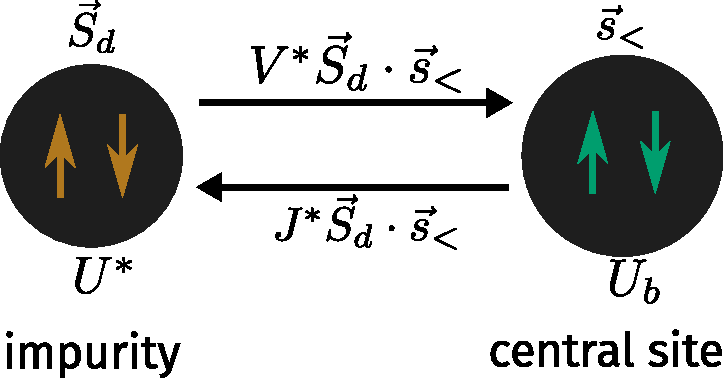
\includegraphics[width=\textwidth]{./figures/zeromode.pdf}
\end{minipage}
\hspace*{\fill}
\begin{minipage}{0.55\textwidth}
\only<2>{
\[\Delta J>0,\Delta V>0,\Delta U <0, ~ ~ ~ J^* \gg V^* \gg U^*\]
\[\frac{1}{\sqrt 2}\left(\ket{\uparrow,\downarrow} - \ket{\downarrow,\uparrow}\right) \]
}
\only<3>{
\[\Delta J<0,\Delta V<0,\Delta U >0, ~ ~ ~ J^* = V^* = 0, U^* \geq 0\]
\[\left\{\ket{\uparrow}, \ket{\downarrow}\right\} \otimes \left\{\ket{0}, \ket{2}\right\} \]
}
\only<4>{
\[\Delta J<0,\Delta V<0,\Delta U < 0, ~ ~ ~ J^* = V^* = U^* = 0\]
\[\left\{\ket{\uparrow}, \ket{\downarrow}, \ket{0}, \ket{2} \right\} \otimes \left\{\ket{0}, \ket{2}\right\} \]
}
\only<5>{
\[J^* < U^* < V^*\]
\[\frac{c}{\sqrt 2}\left(\ket{\uparrow,\downarrow} - \ket{\downarrow,\uparrow}\right) + \frac{\sqrt{1 - c^2}}{\sqrt 2}\left(\ket{2,0} + \ket{0,2}\right)\]
}
\end{minipage}
\end{frame}

\section{Evolution of two-site ground state and correlations across the transition}
\label{transition}

\begin{frame}[noframenumbering]{Overlap of ground state against spin singlet and charge triplet zero states}
	\centering
\only<1>{\(J_0/D_0 = 10^{-4}\)

\vspace*{-20pt}
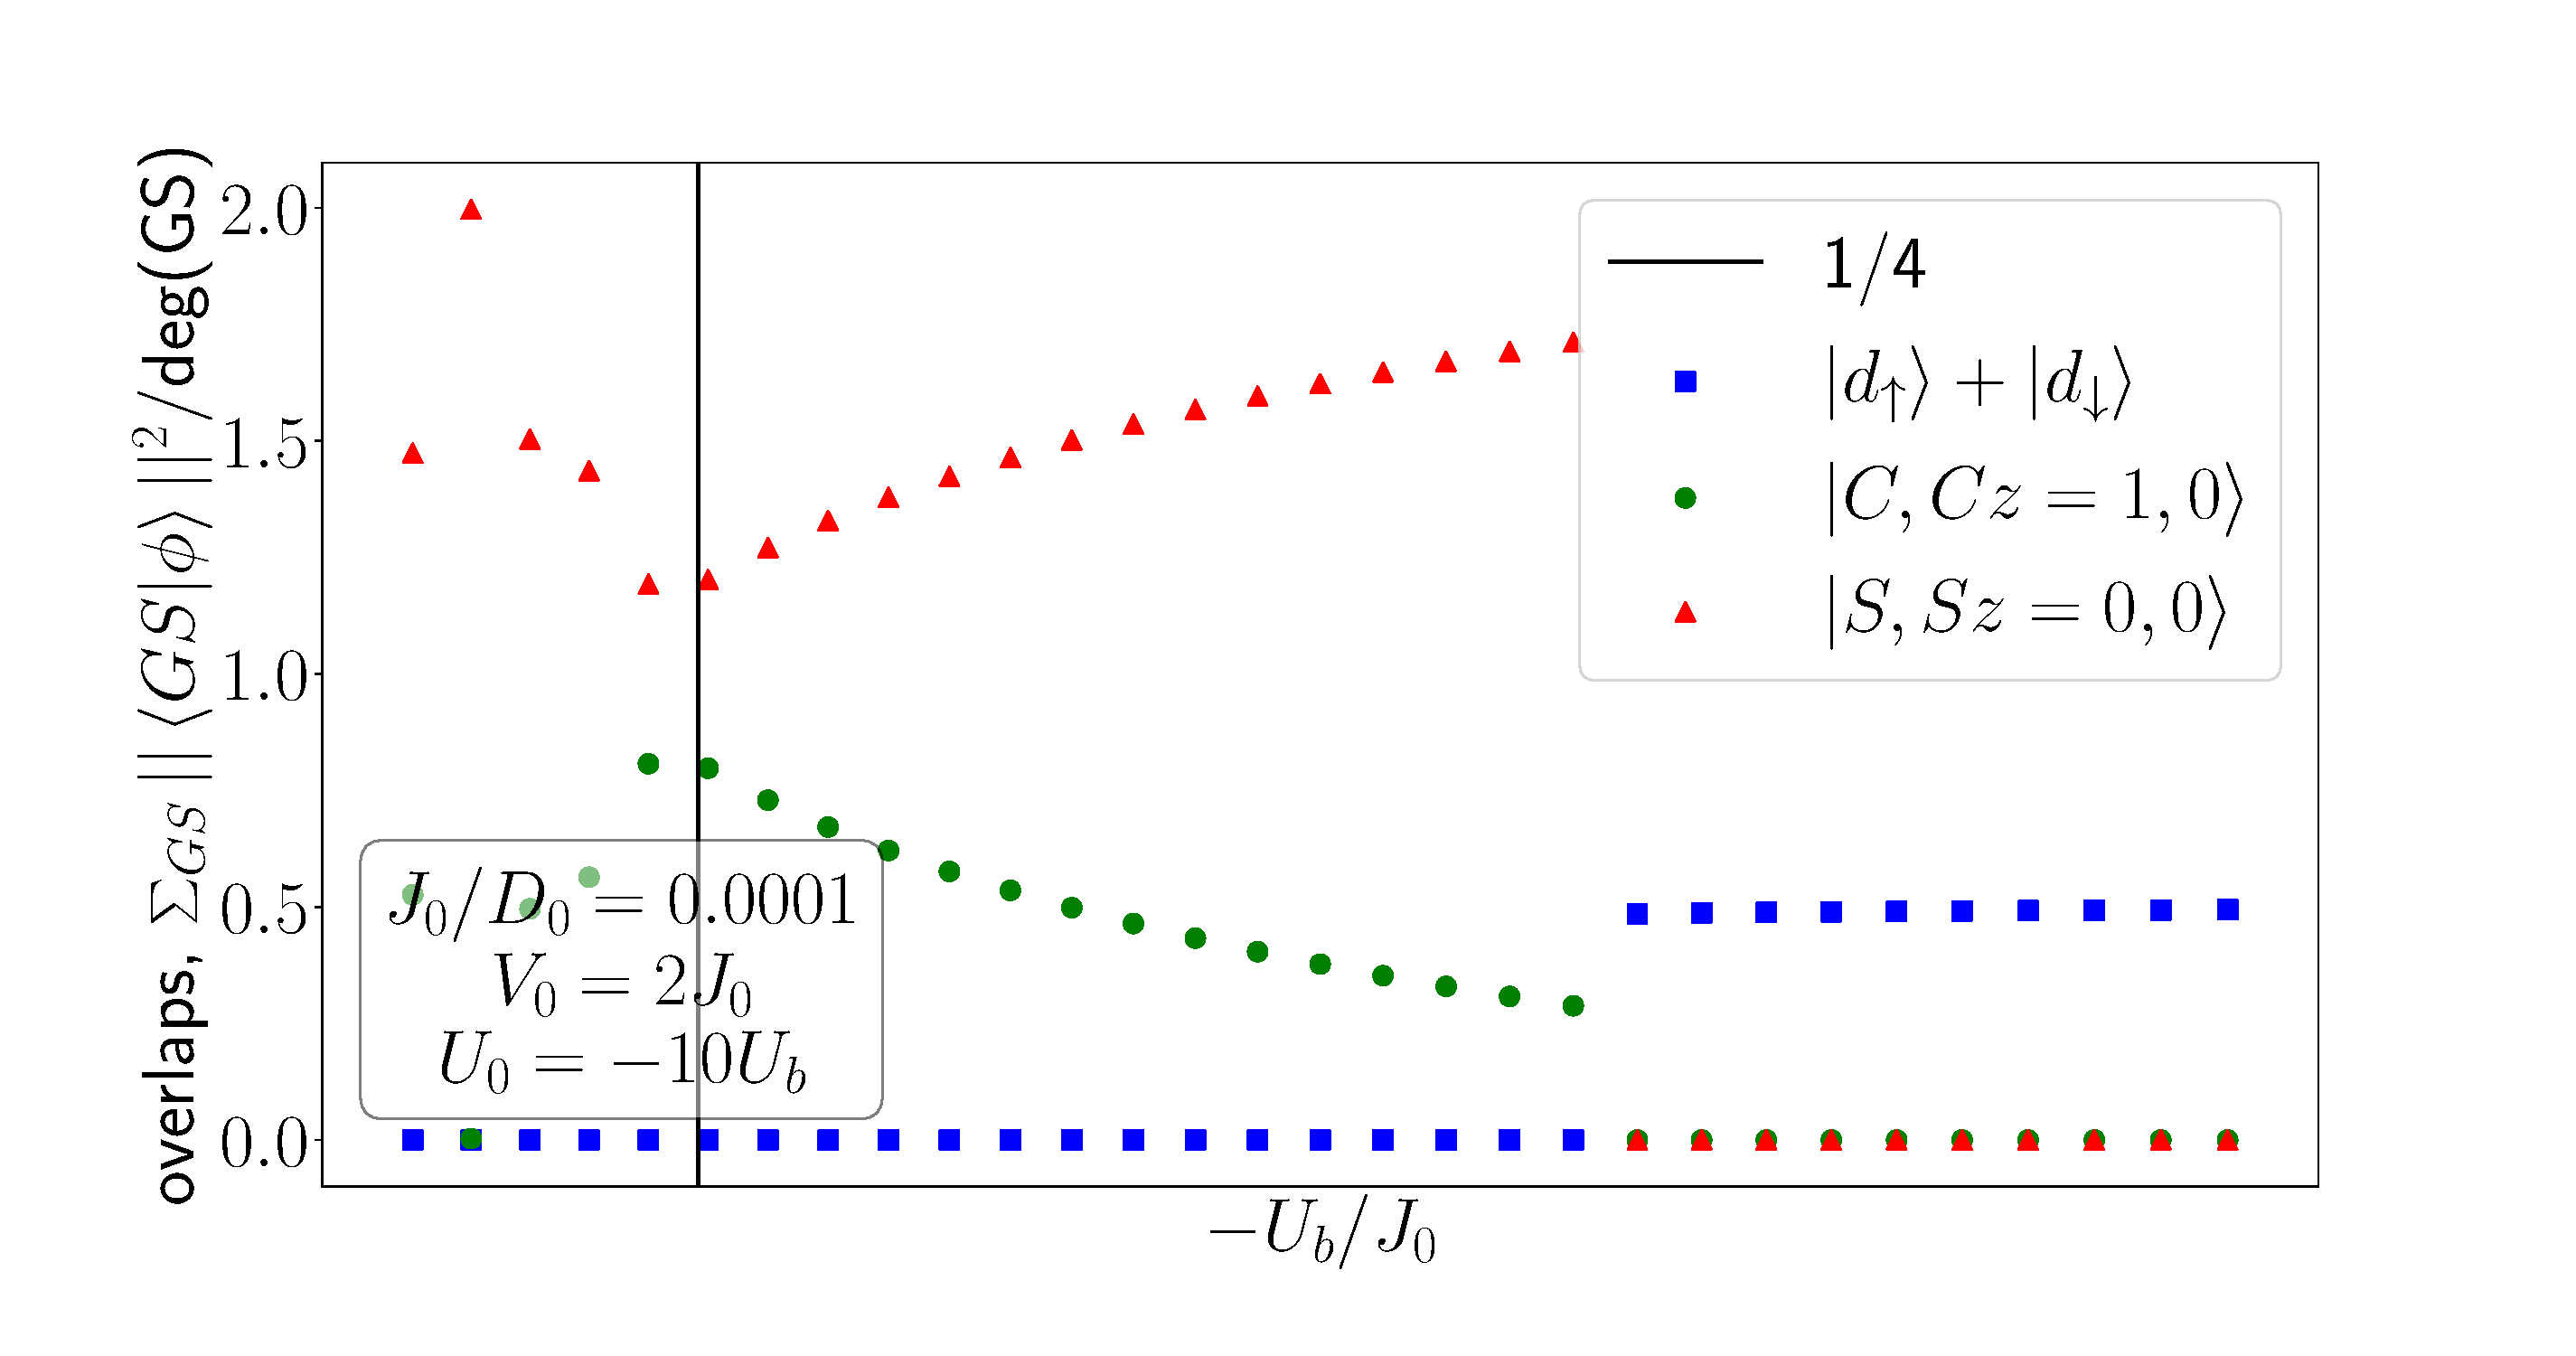
\includegraphics[width=\textwidth]{./figures/overlaps_gs-J=0.100.pdf}
}

\only<2>{\(J_0/D_0 = 10^{-2}\)

\vspace*{-20pt}
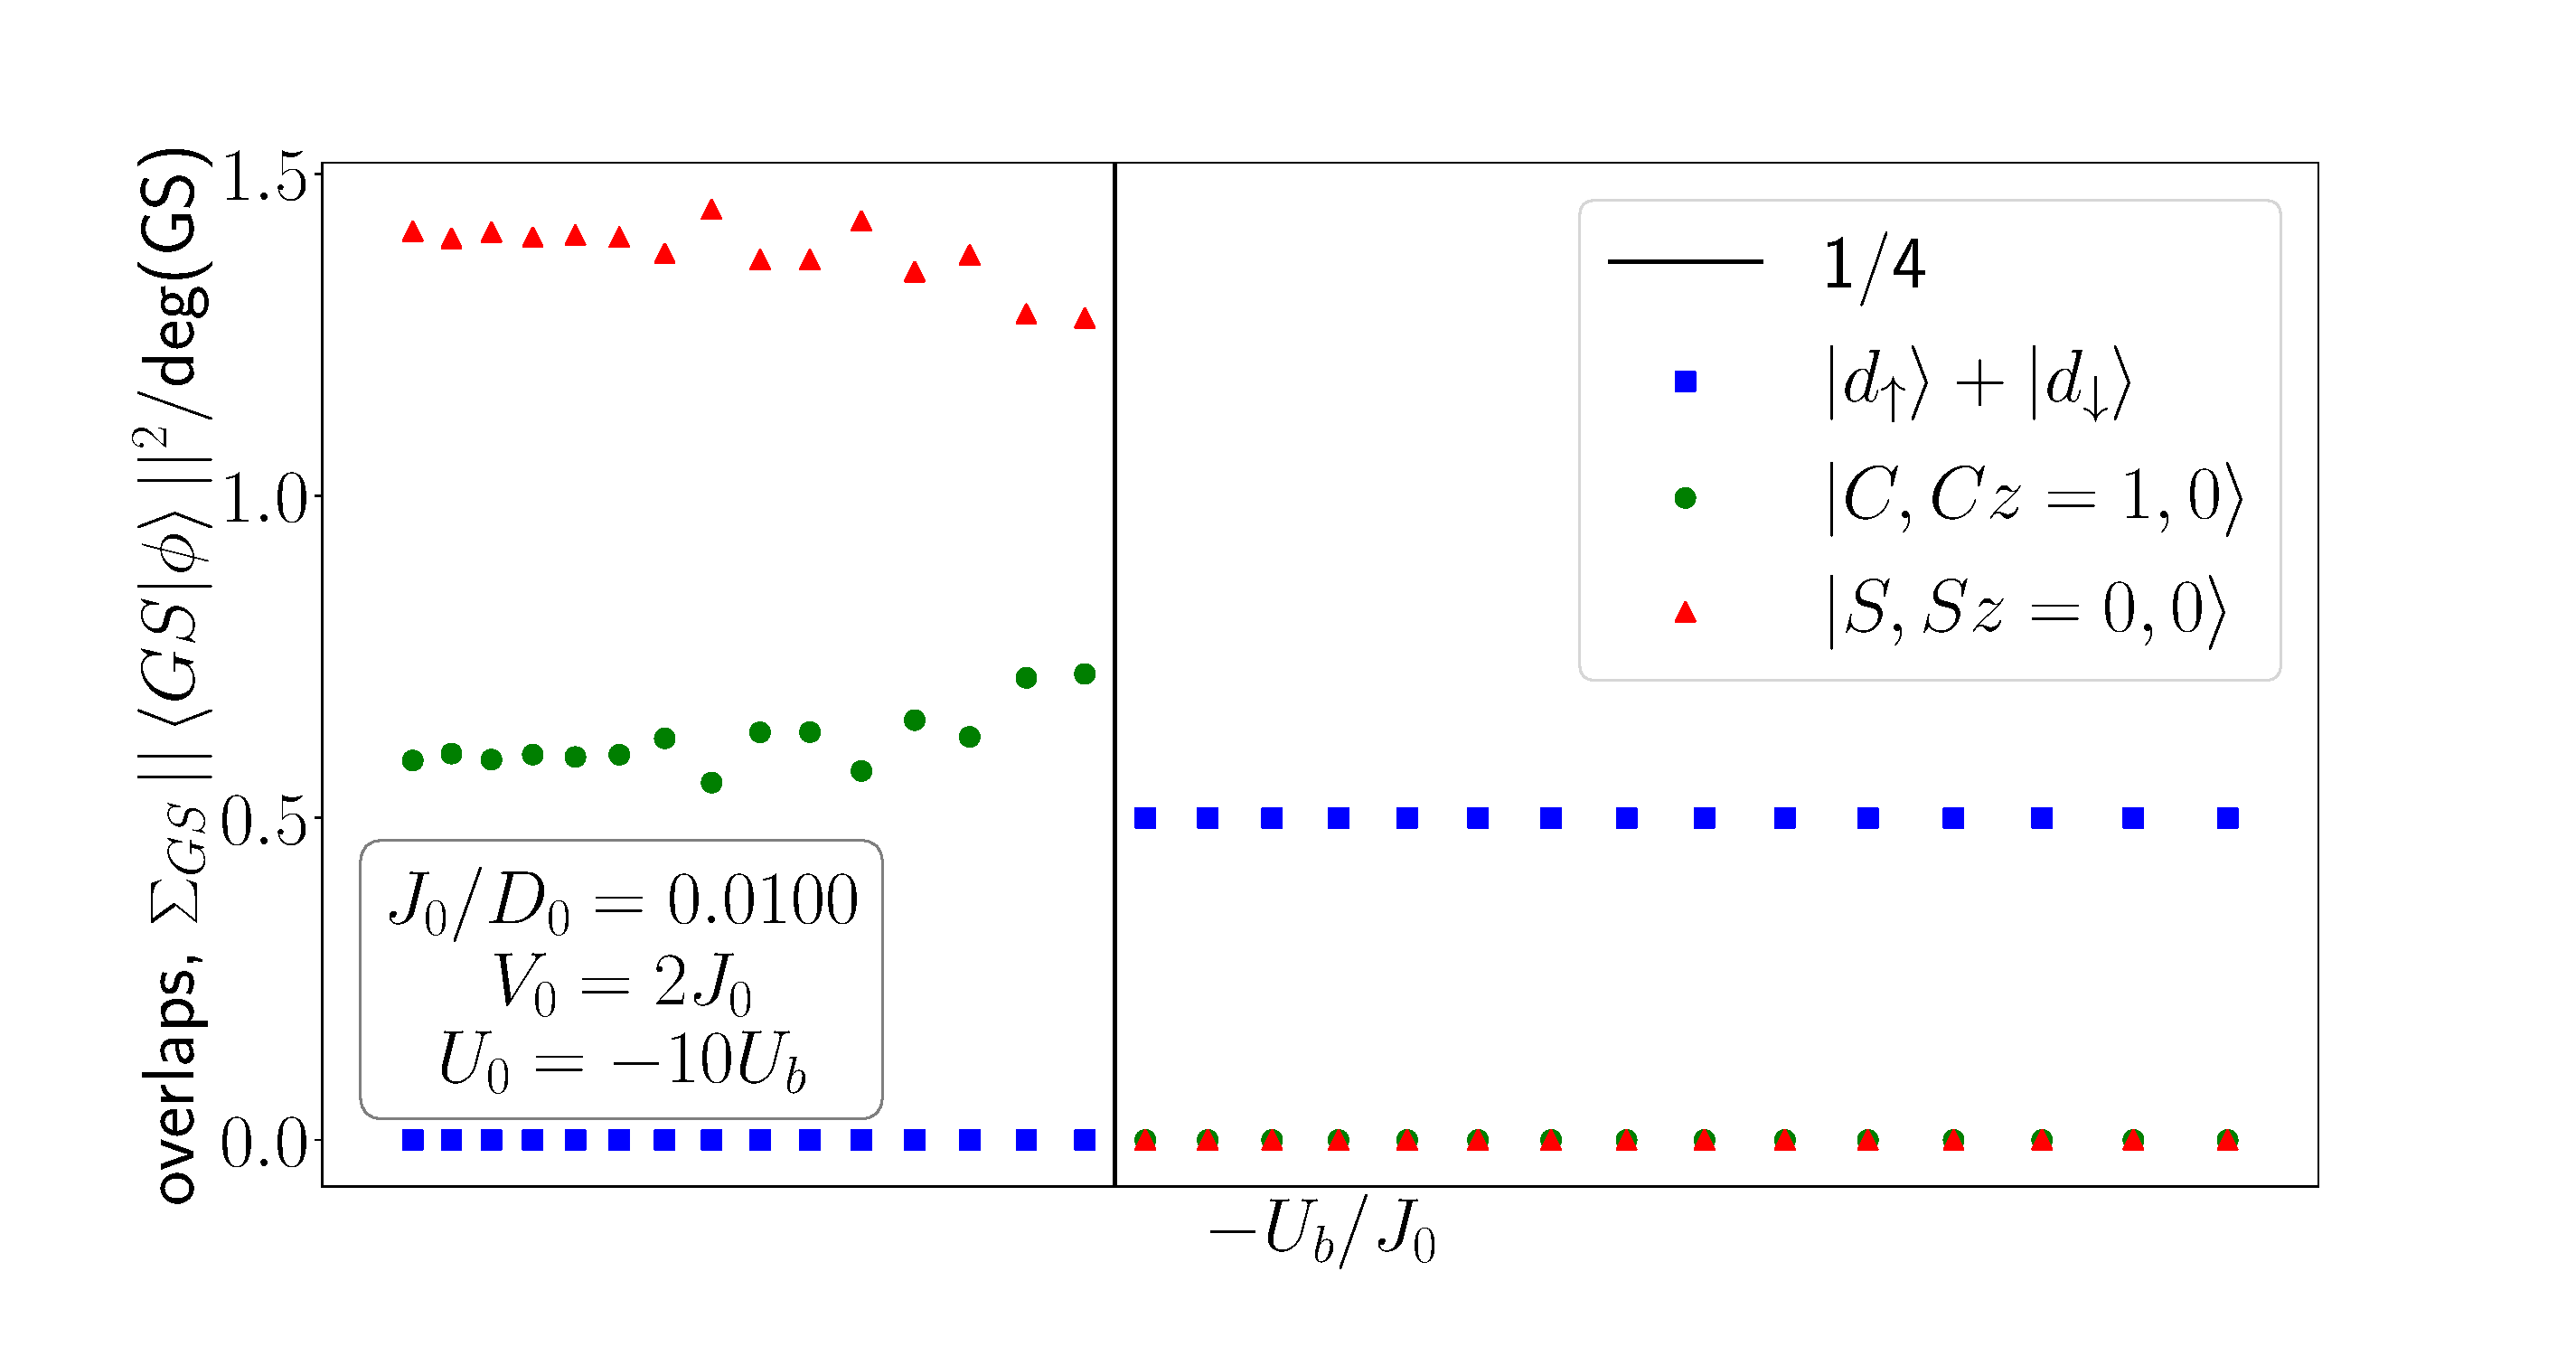
\includegraphics[width=\textwidth]{./figures/overlaps_gs-J=10.000.pdf}}

\only<3>{\(J_0/D_0 = 10^{-1}\)

\vspace*{-20pt}
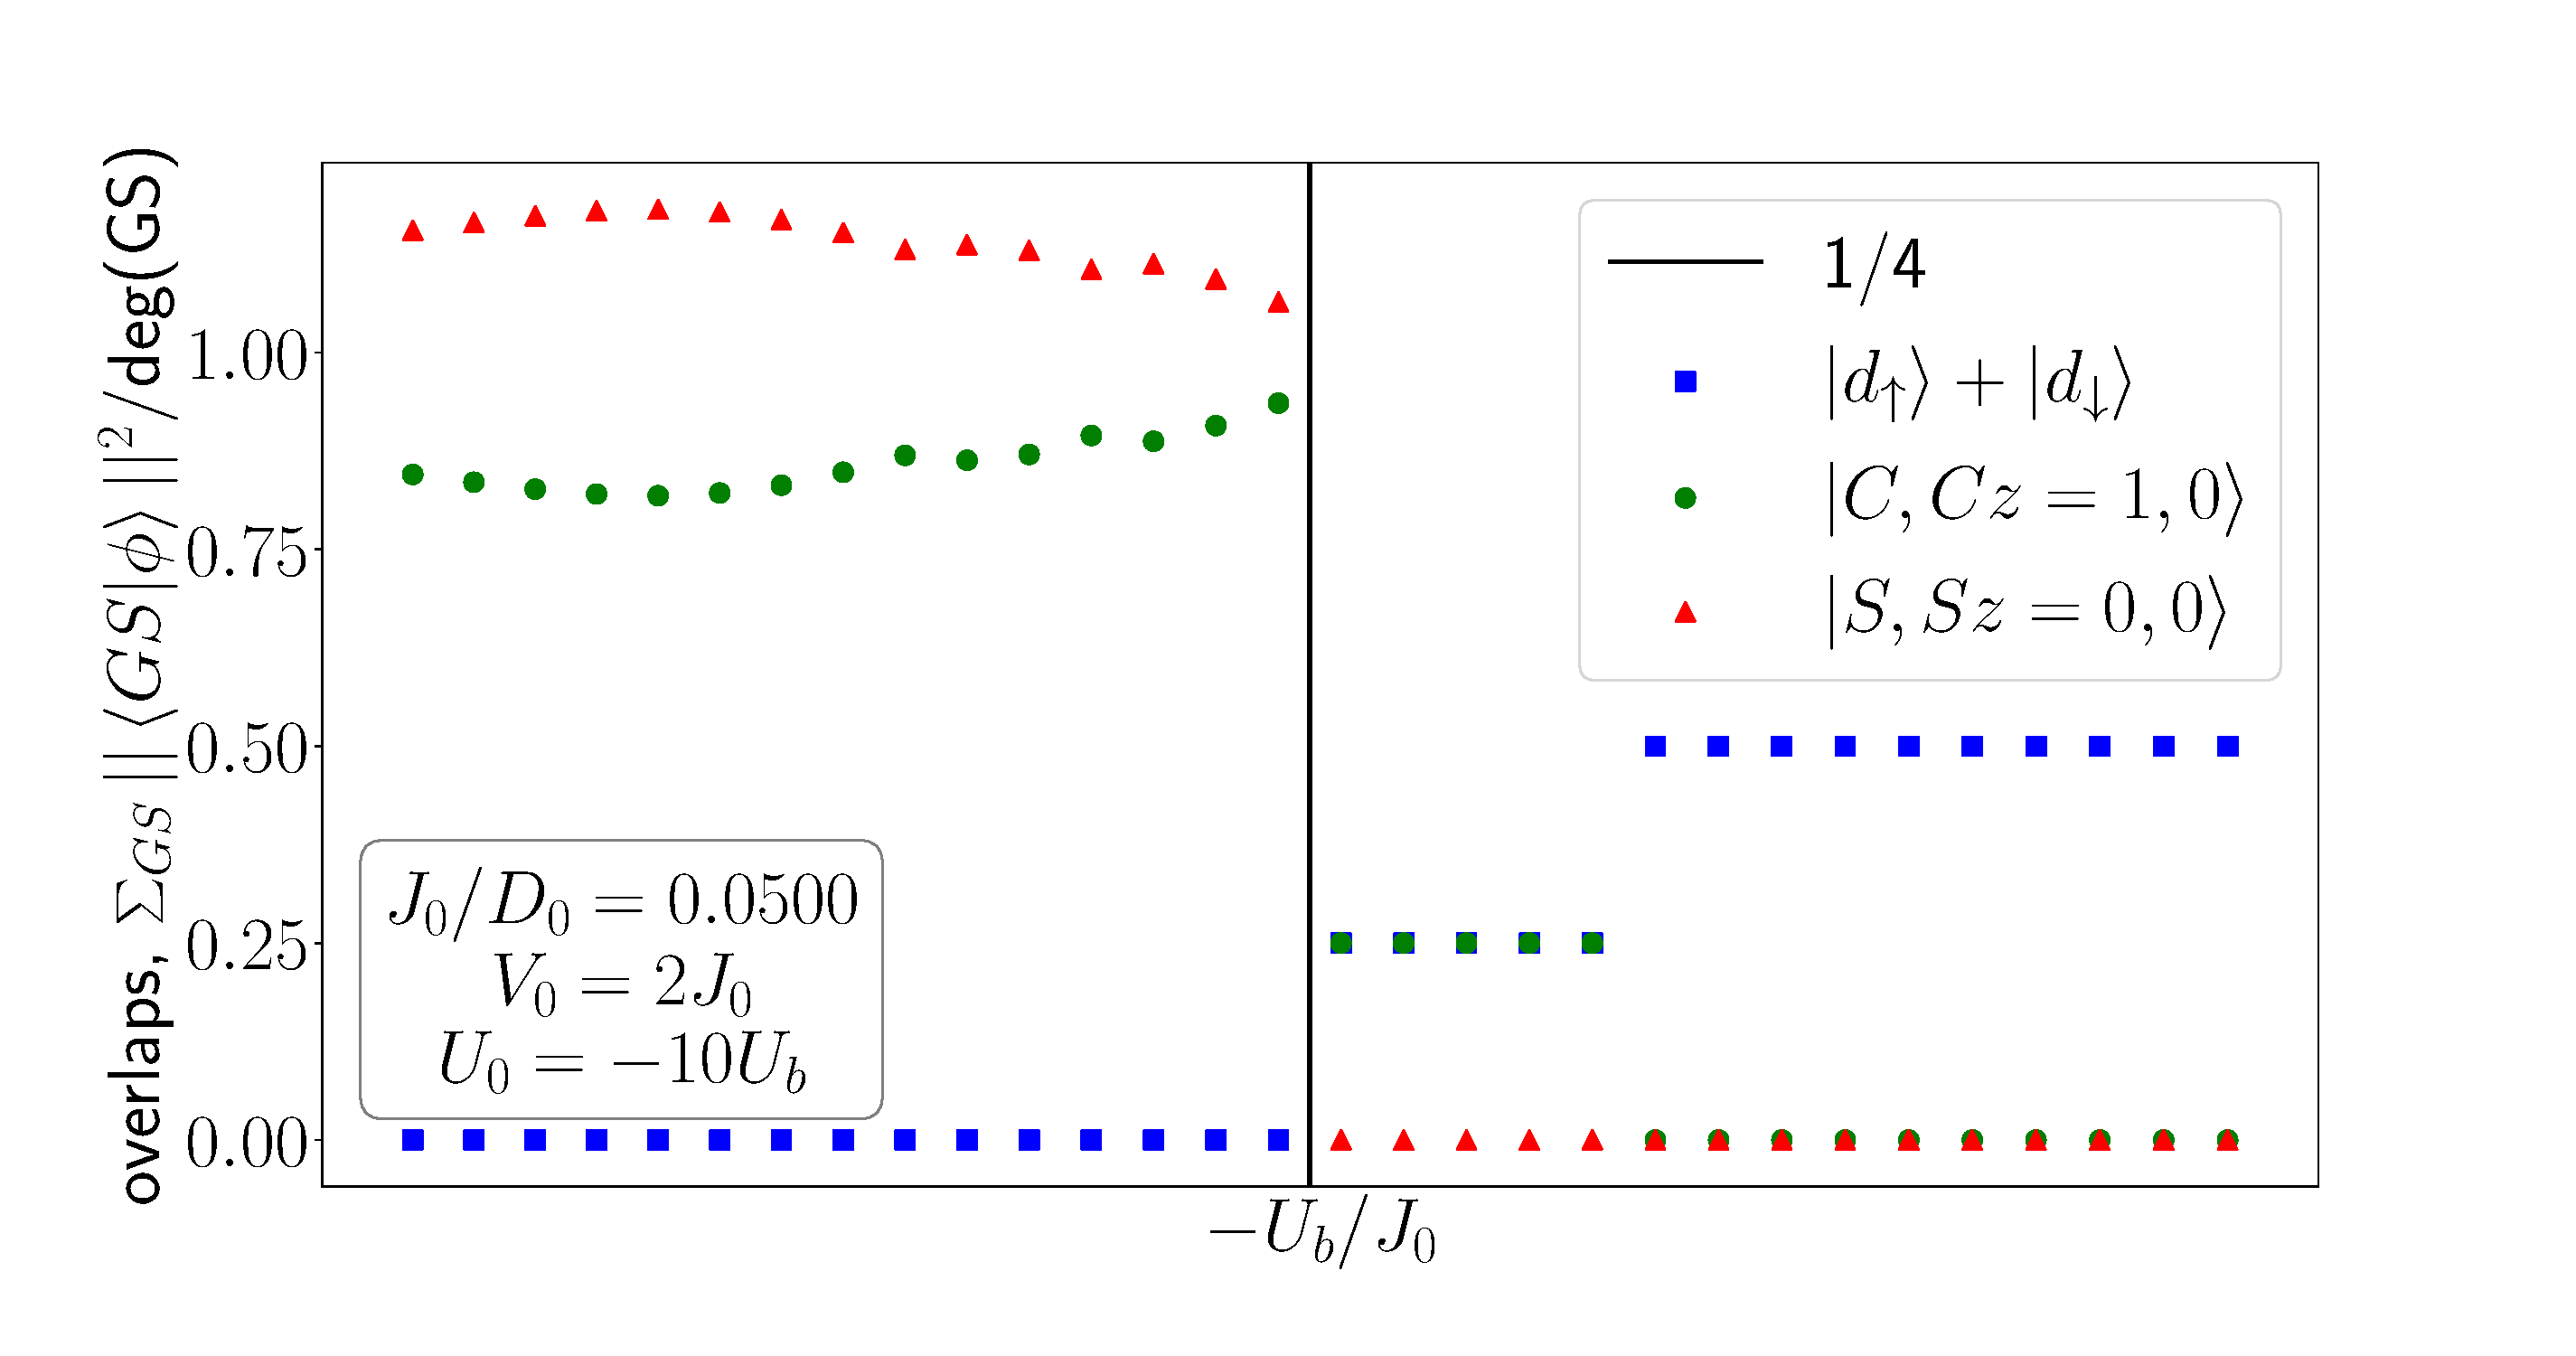
\includegraphics[width=\textwidth]{./figures/overlaps_gs-J=50.000.pdf}}

\end{frame}

\begin{frame}[noframenumbering]{Spin and charge correlations in ground state}
	\centering
\only<1>{\(J_0/D_0 = 10^{-4}\)

\vspace*{-20pt}
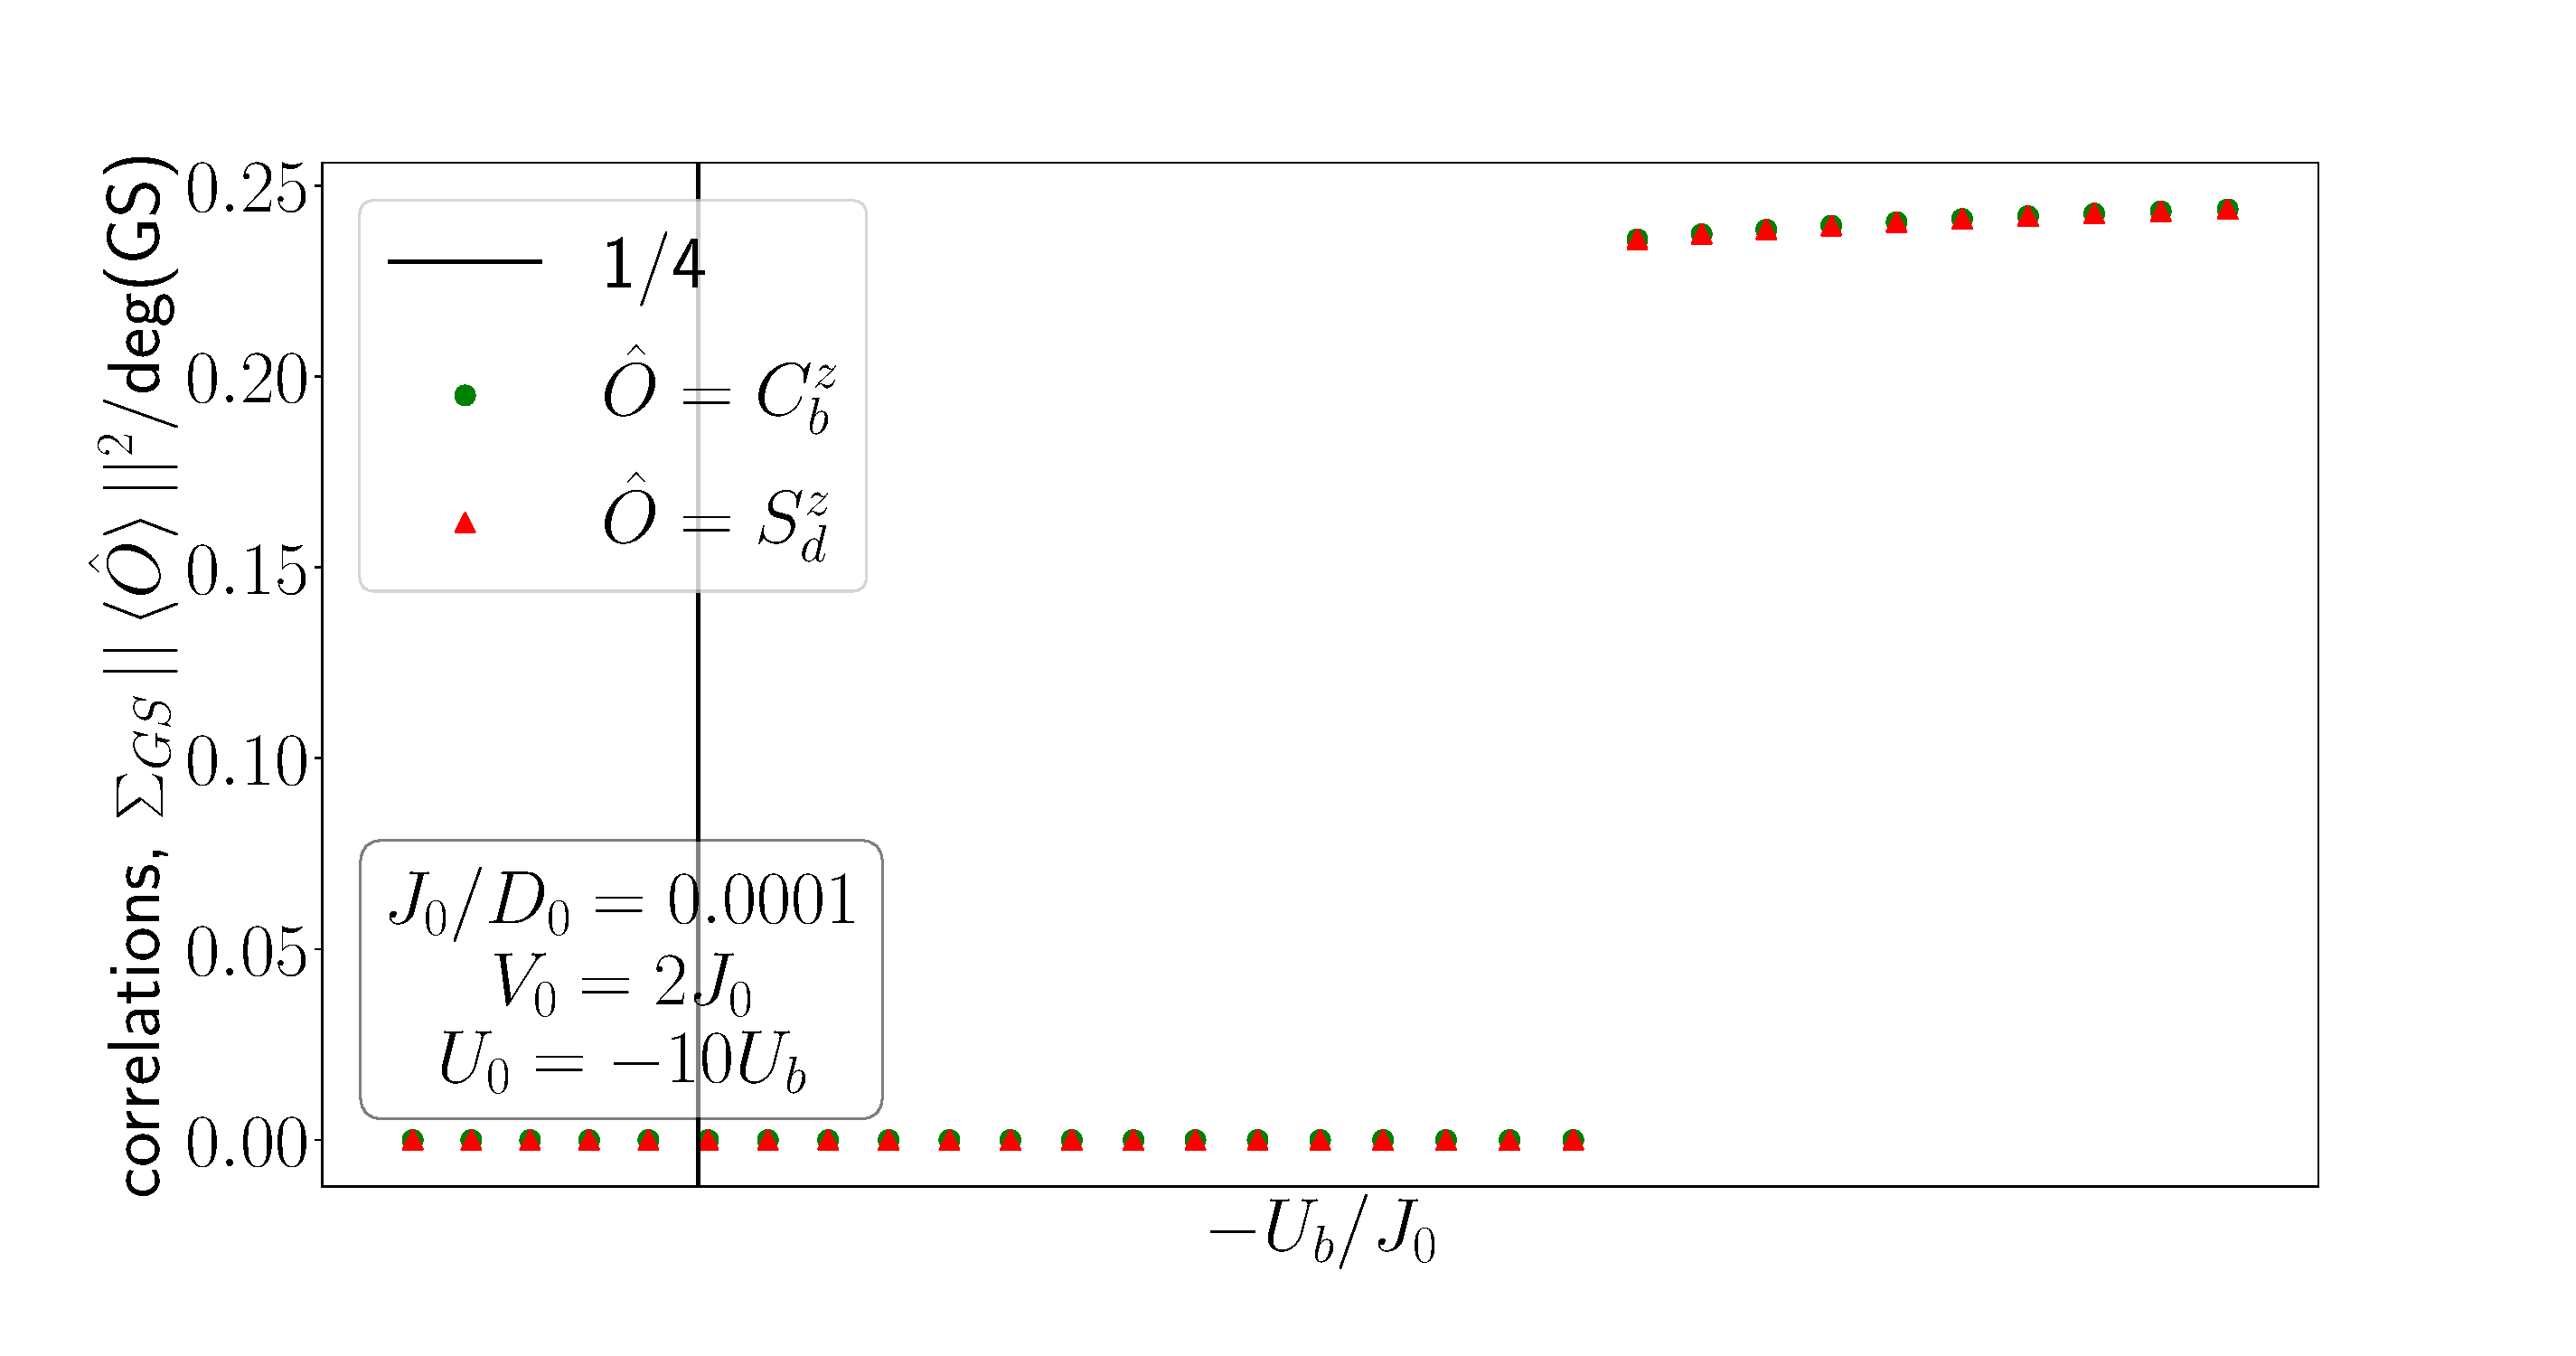
\includegraphics[width=\textwidth]{./figures/corrs_gs-J=0.100.pdf}
}

\only<2>{\(J_0/D_0 = 10^{-2}\)

\vspace*{-20pt}
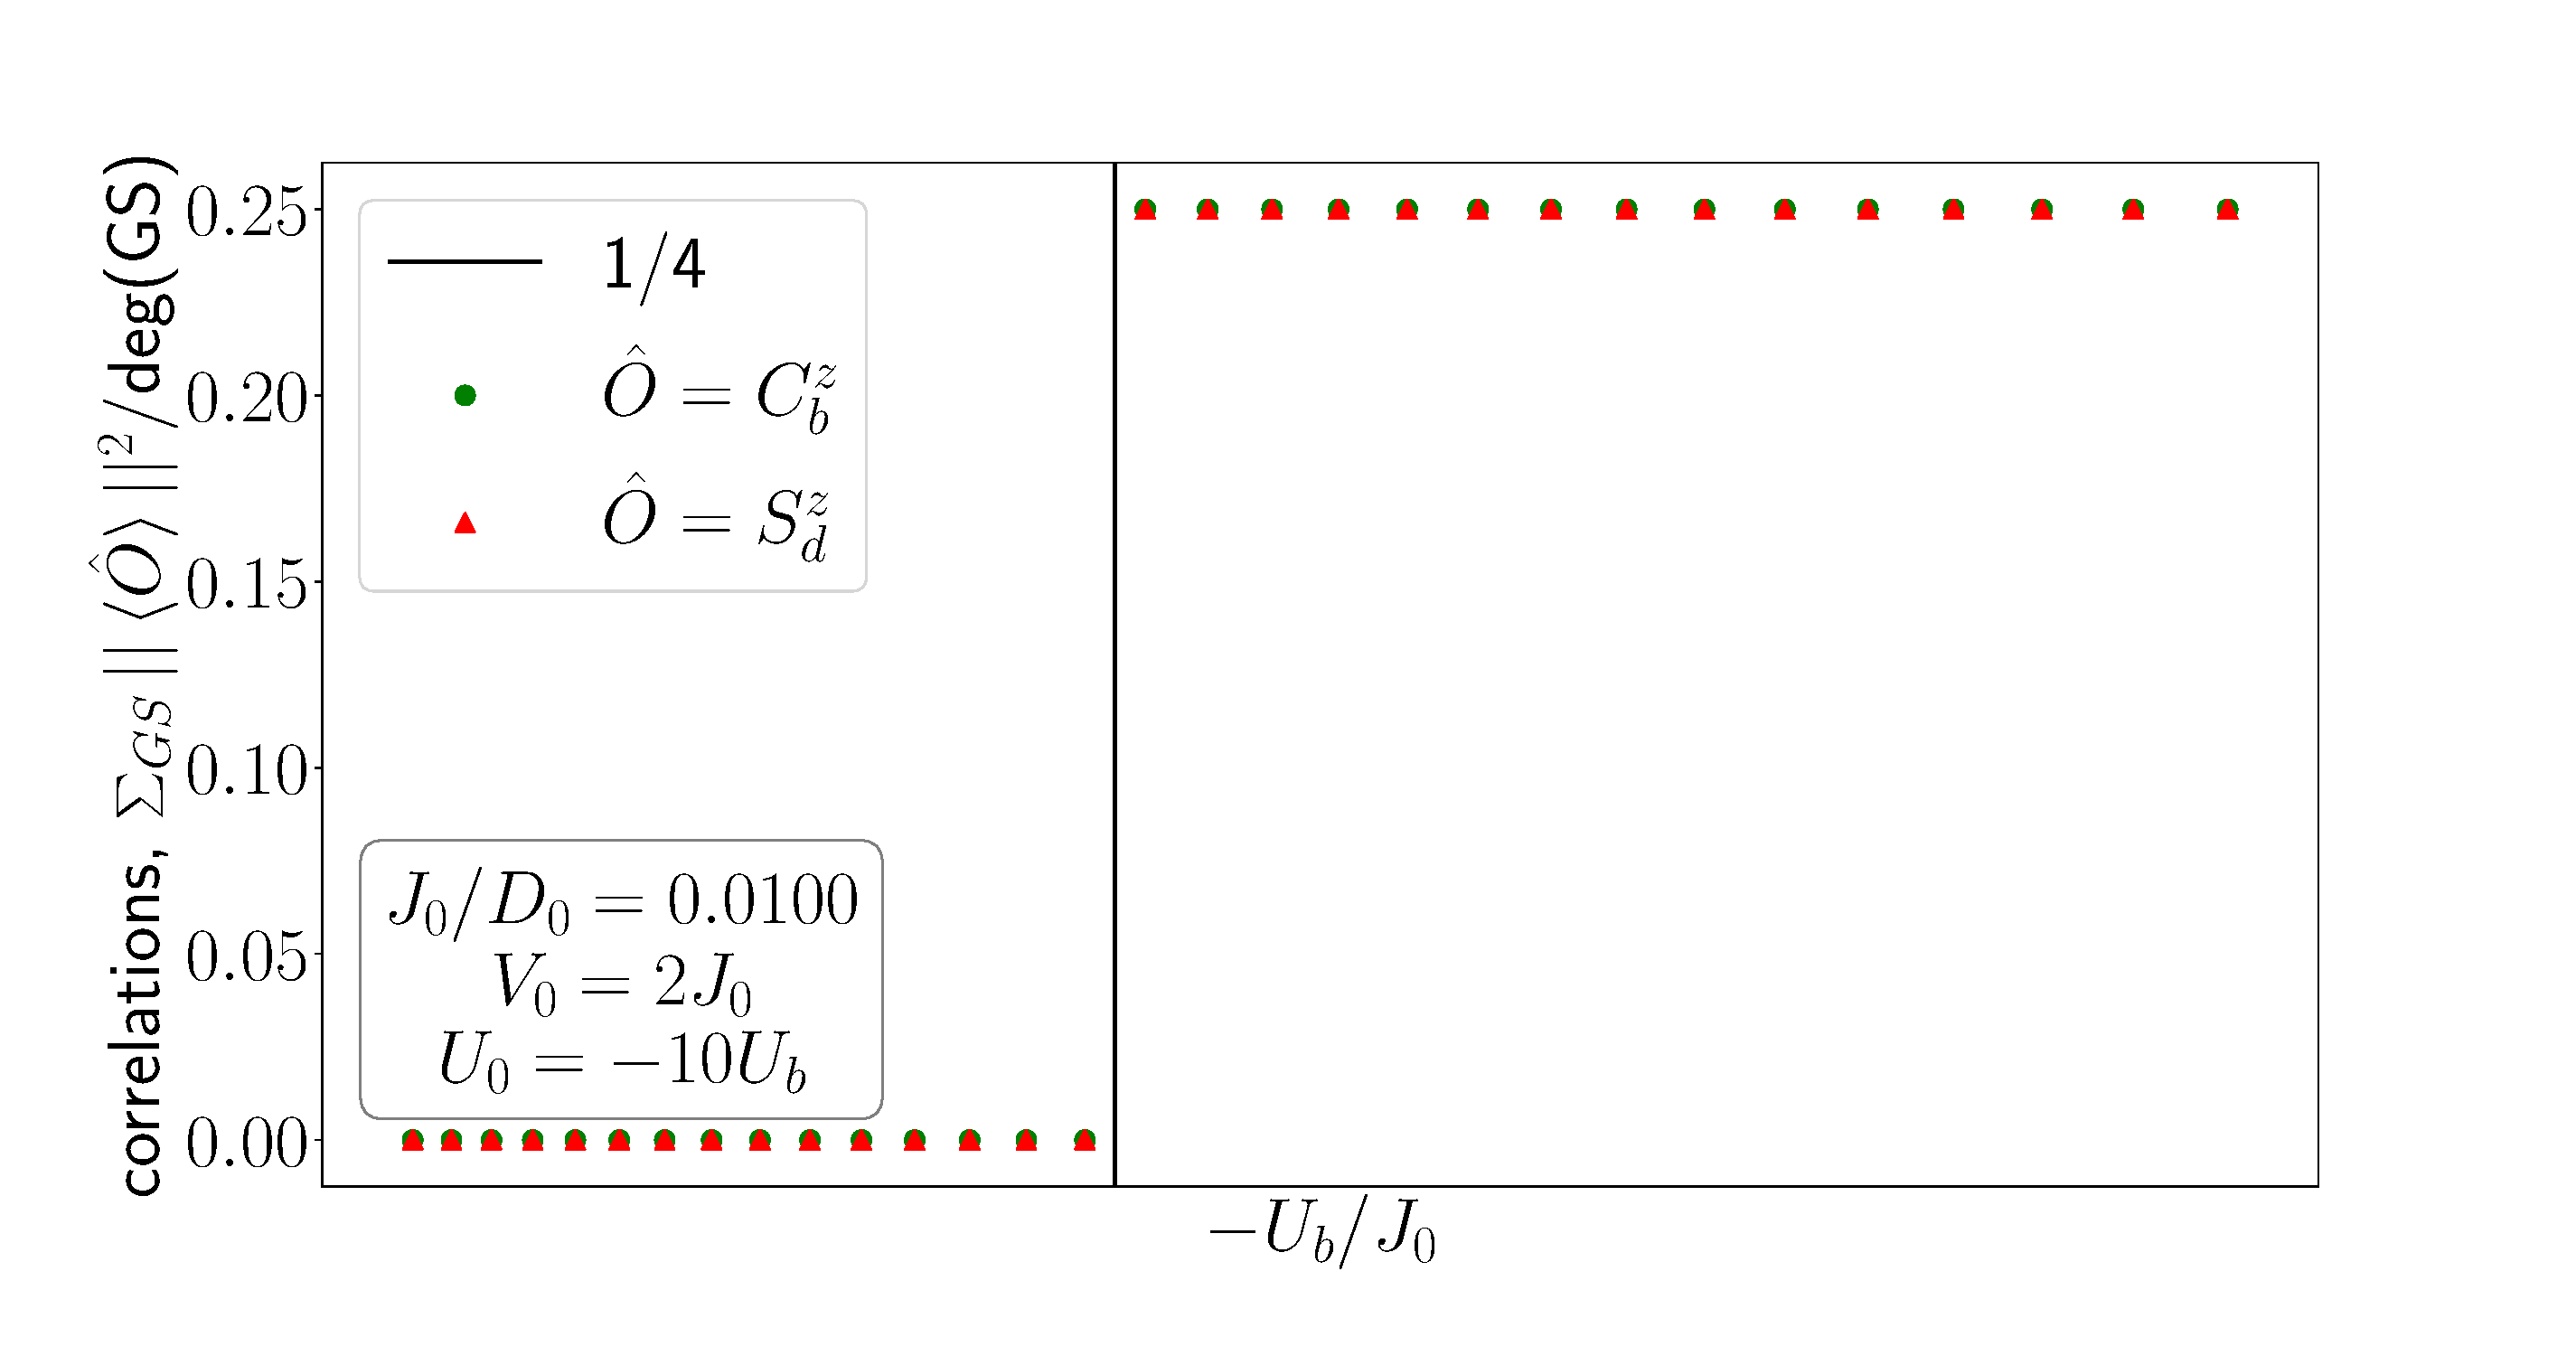
\includegraphics[width=\textwidth]{./figures/corrs_gs-J=10.000.pdf}}

\only<3>{\(J_0/D_0 = 10^{-1}\)

\vspace*{-20pt}
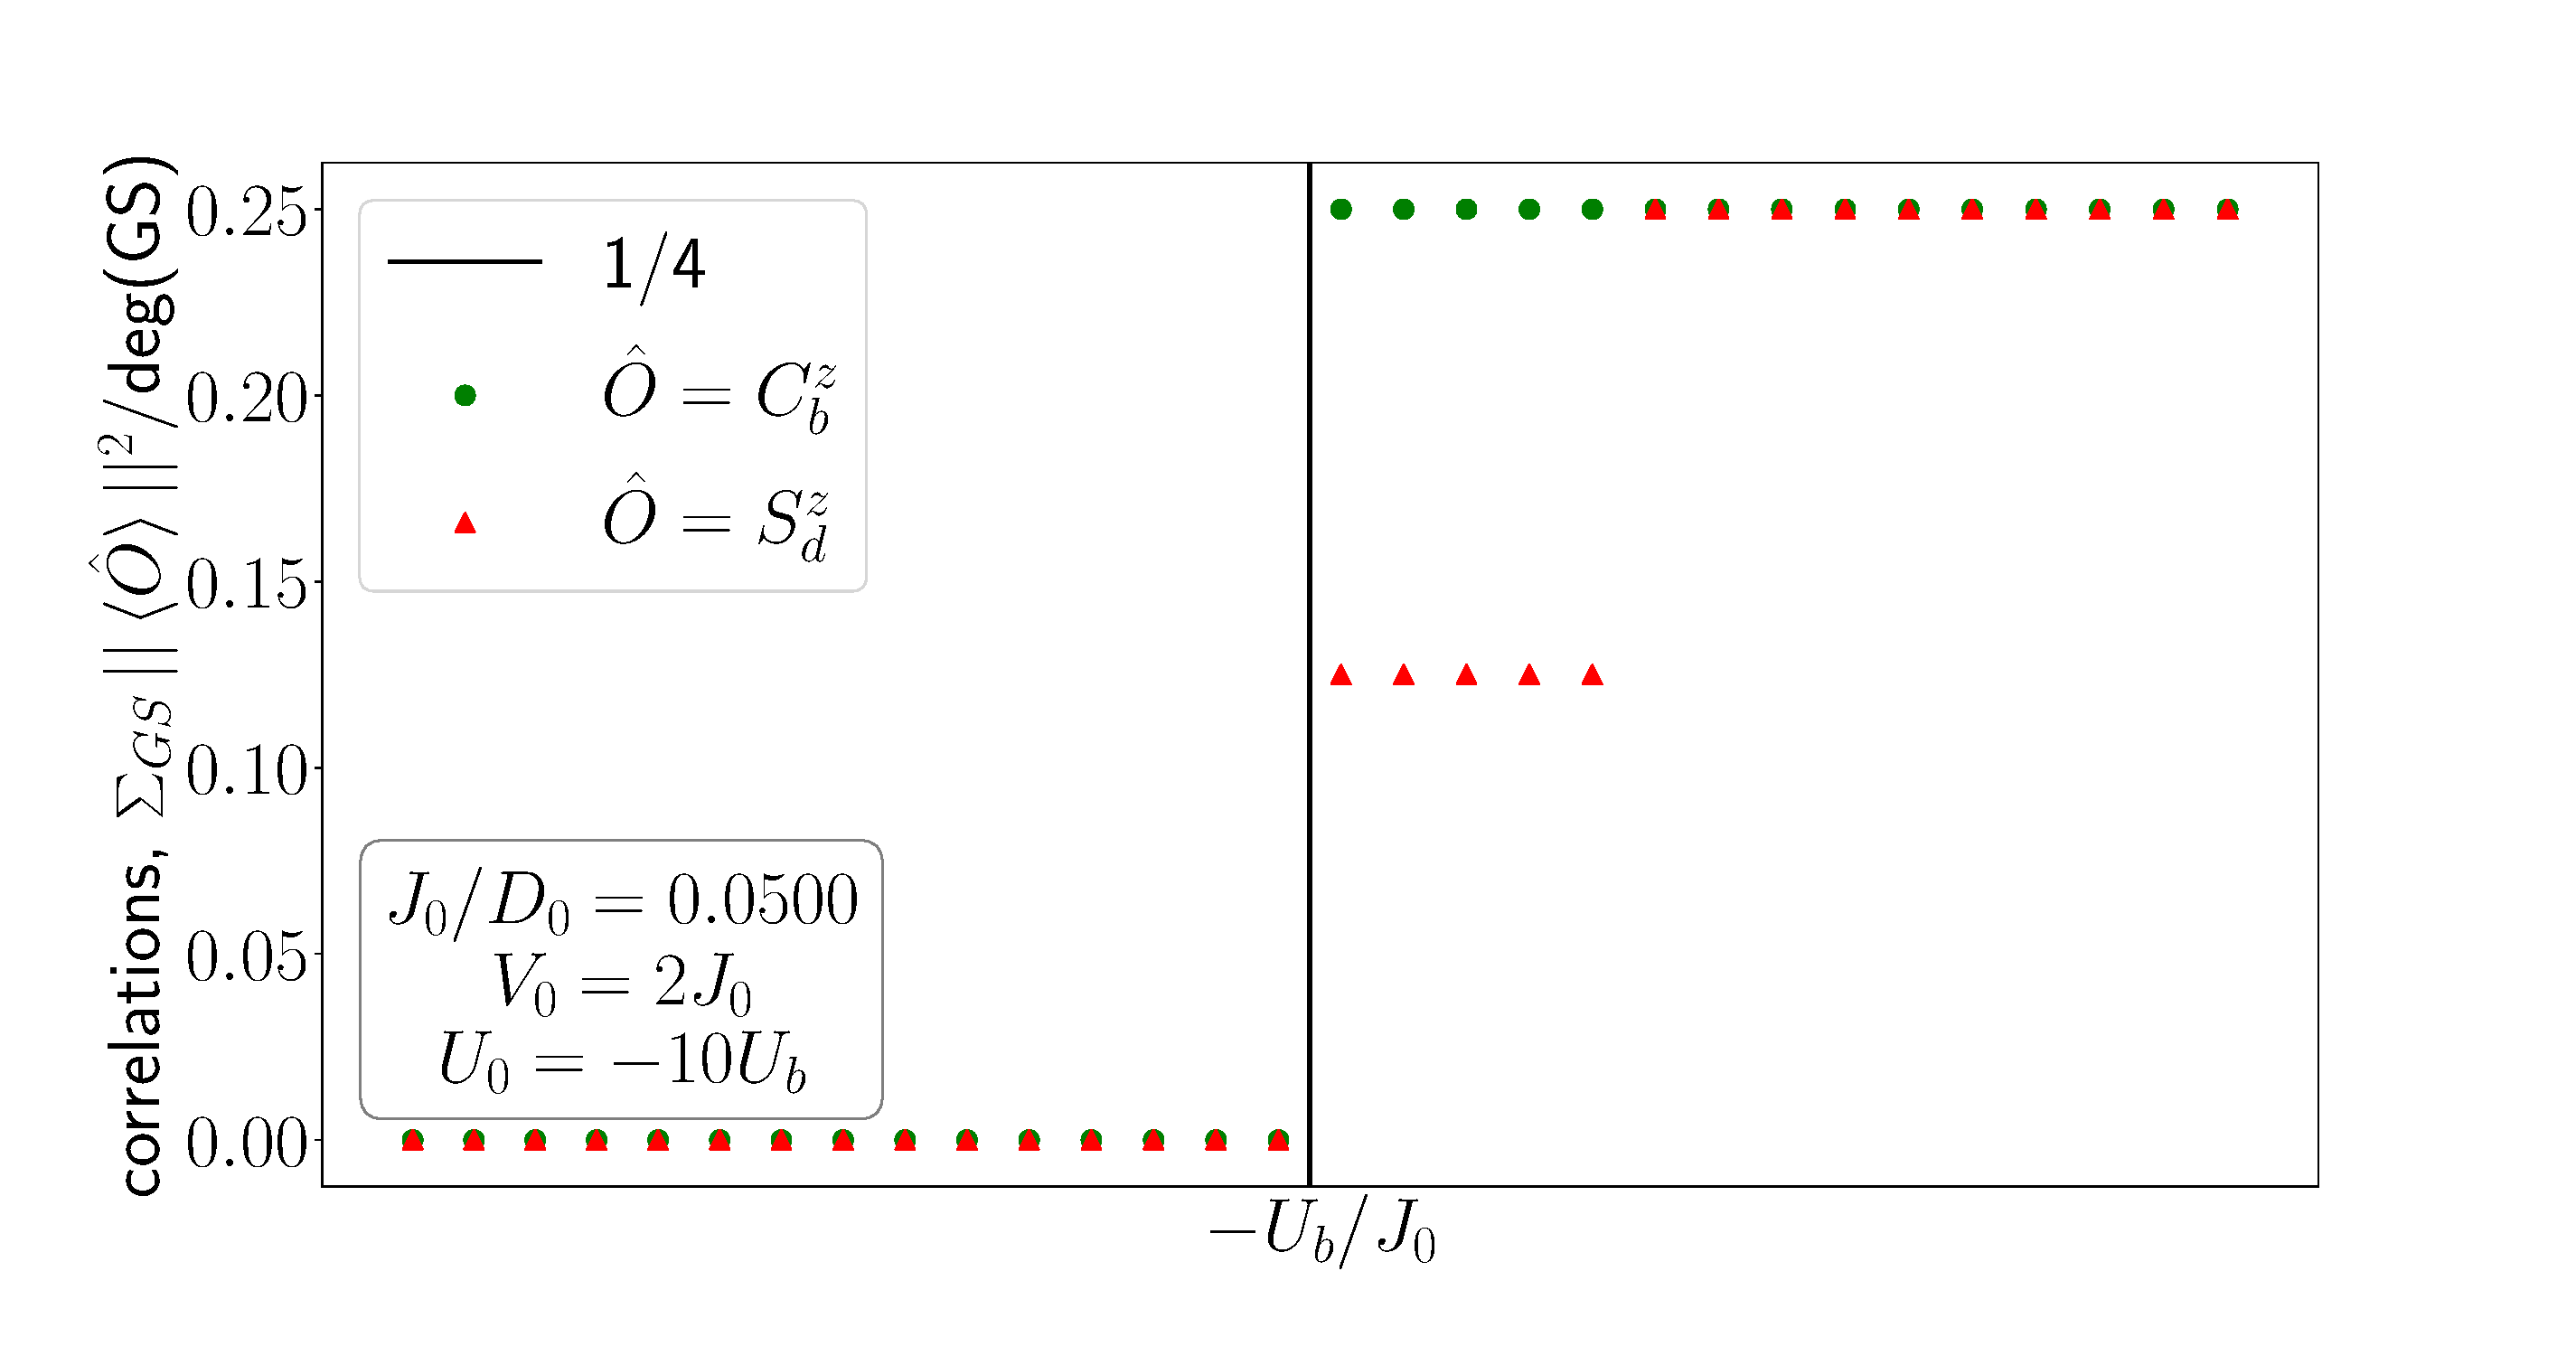
\includegraphics[width=\textwidth]{./figures/corrs_gs-J=50.000.pdf}}

\end{frame}

\begin{frame}[noframenumbering]{Correlation measures: Local Fermi liquid}
\vspace*{20pt}
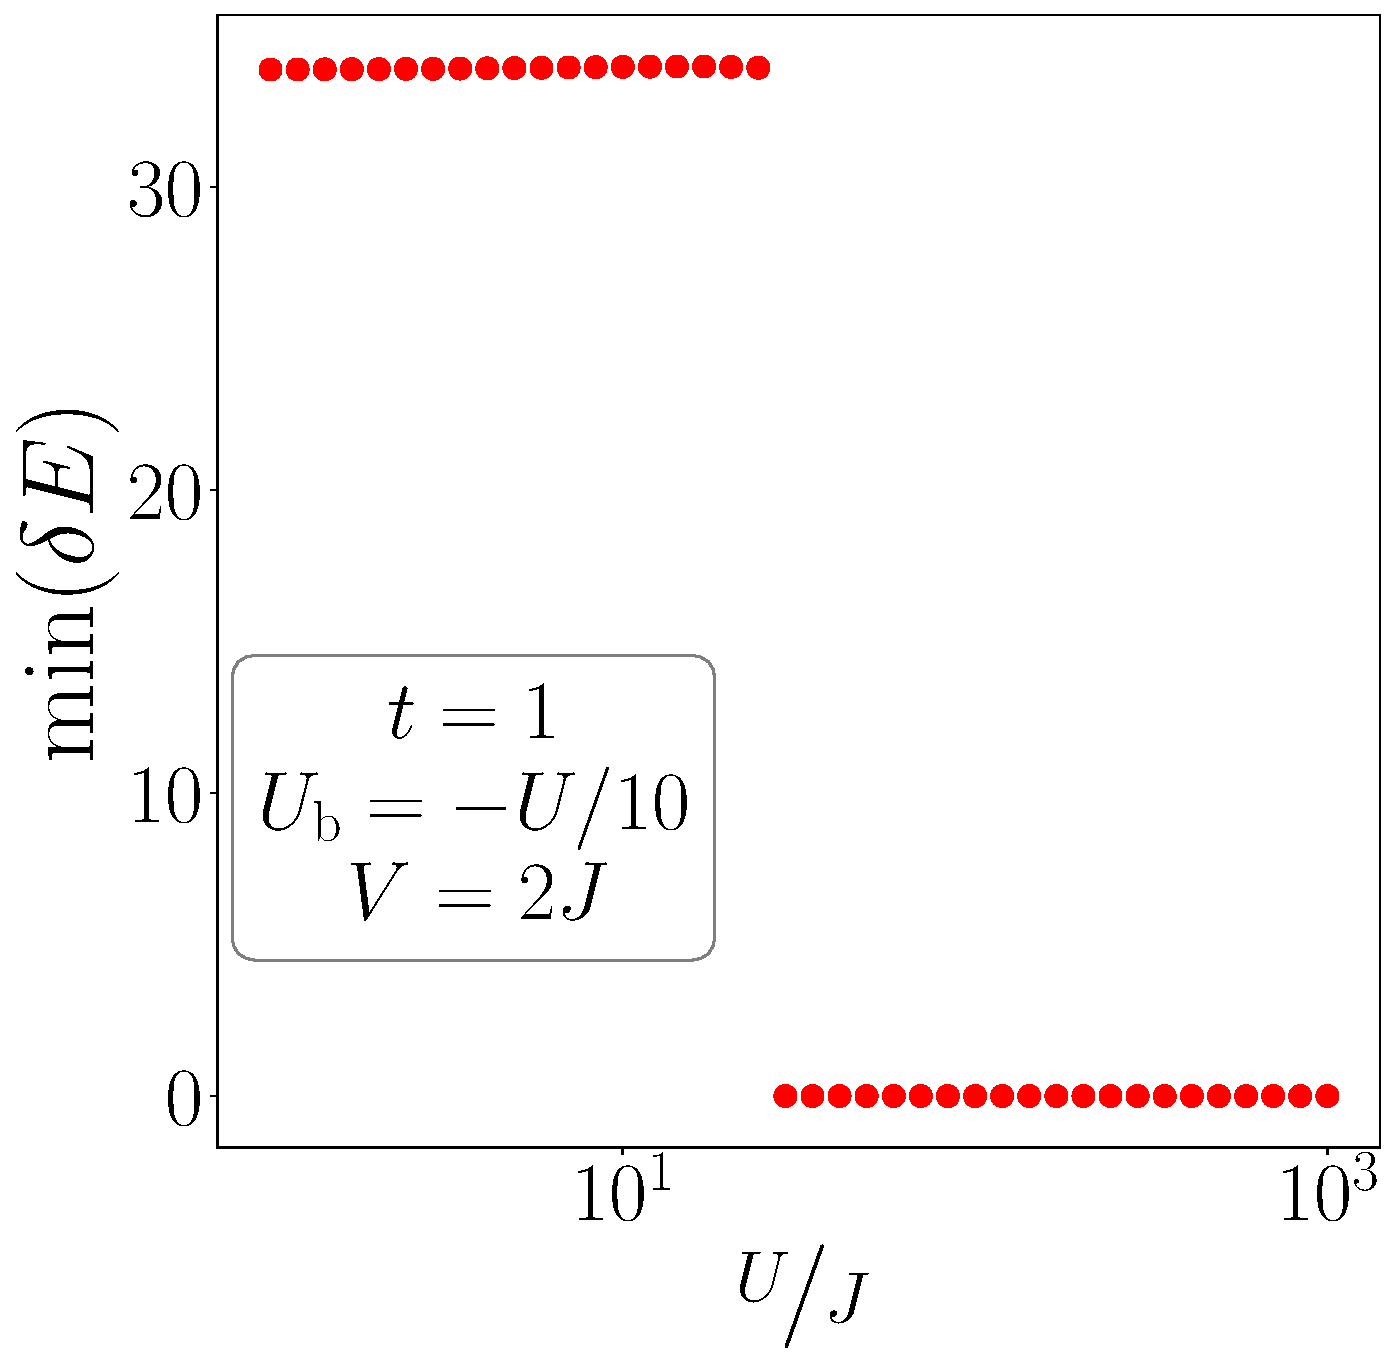
\includegraphics[width=0.49\textwidth]{./figures/gap-t=1.000,J=10.000,0.000,40,V=3J,Ubath=-U_by_10,N=4,U=1.000,1000.000,40.pdf}
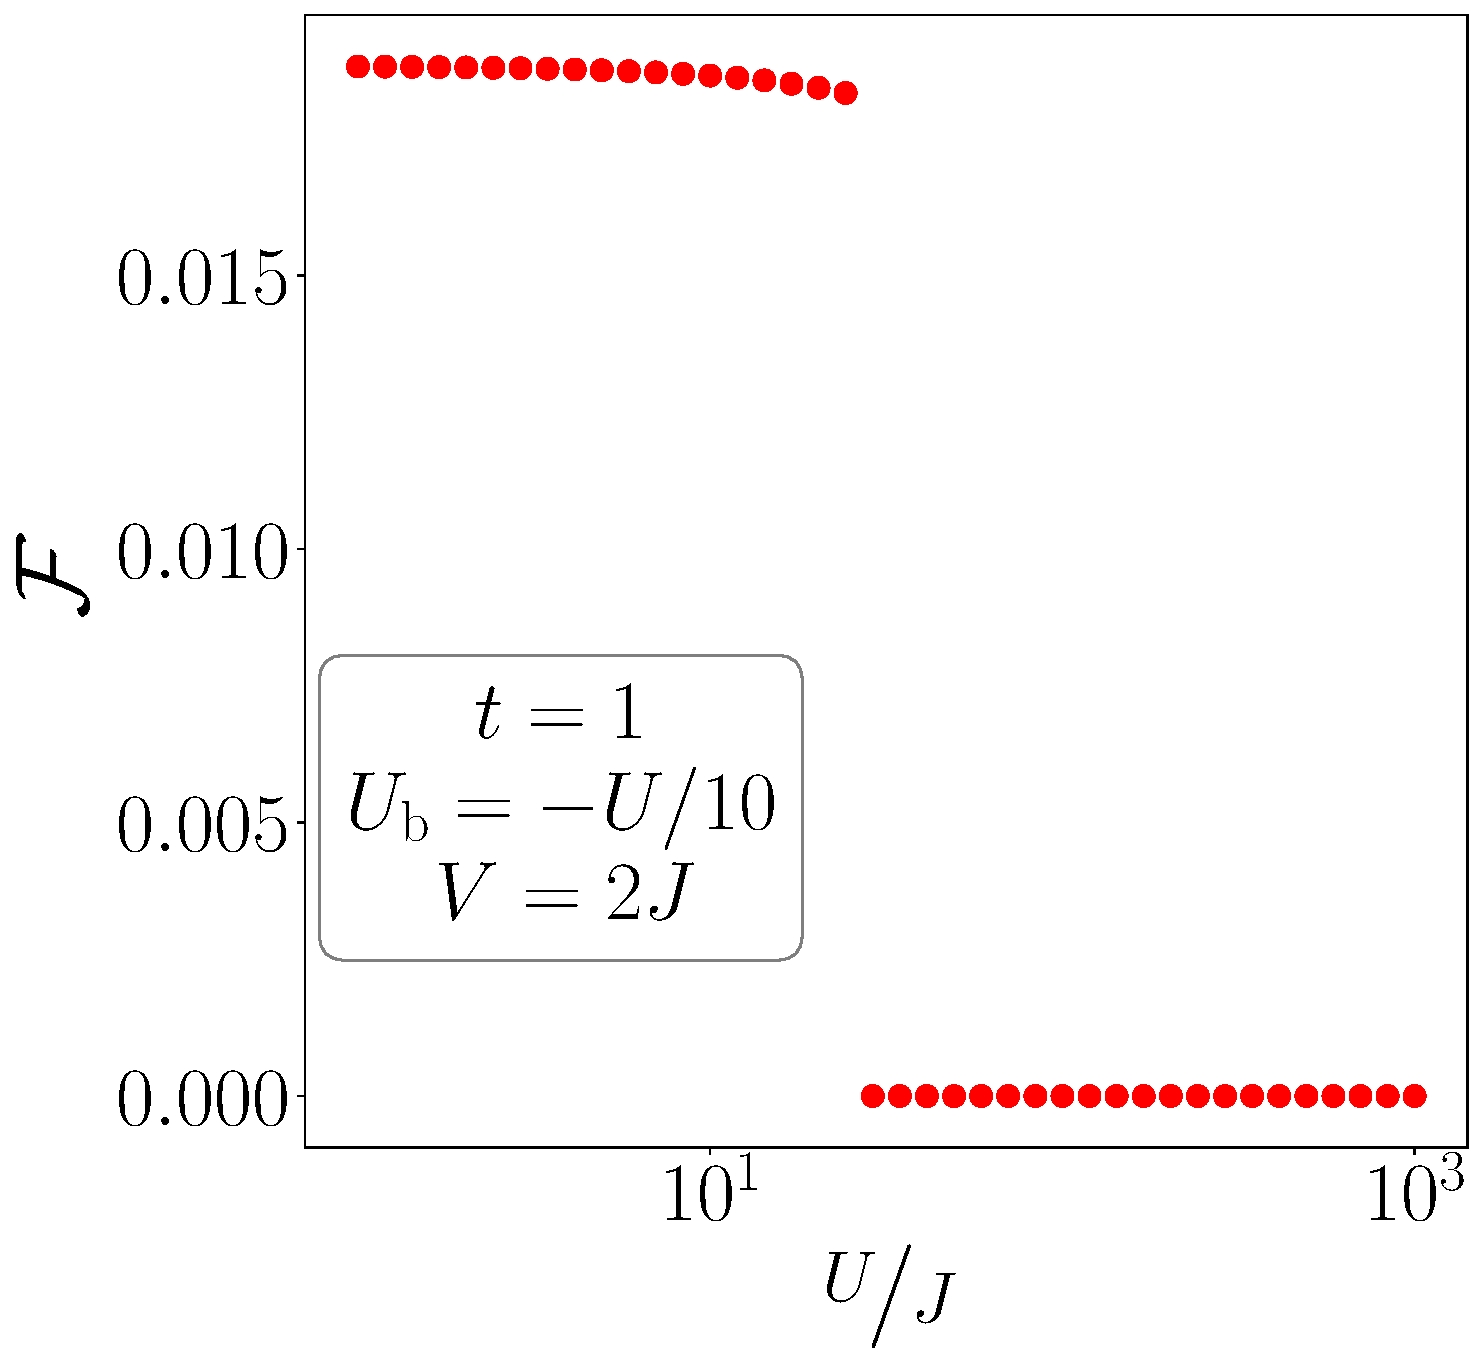
\includegraphics[width=0.49\textwidth]{./figures/lfl-t=1.000,J=10.000,0.000,40,V=3J,Ubath=-U_by_10,N=4,U=1.000,1000.000,40.pdf}
\end{frame}


\begin{frame}[noframenumbering]{Correlation measures: Kondo cloud}
\vspace*{20pt}
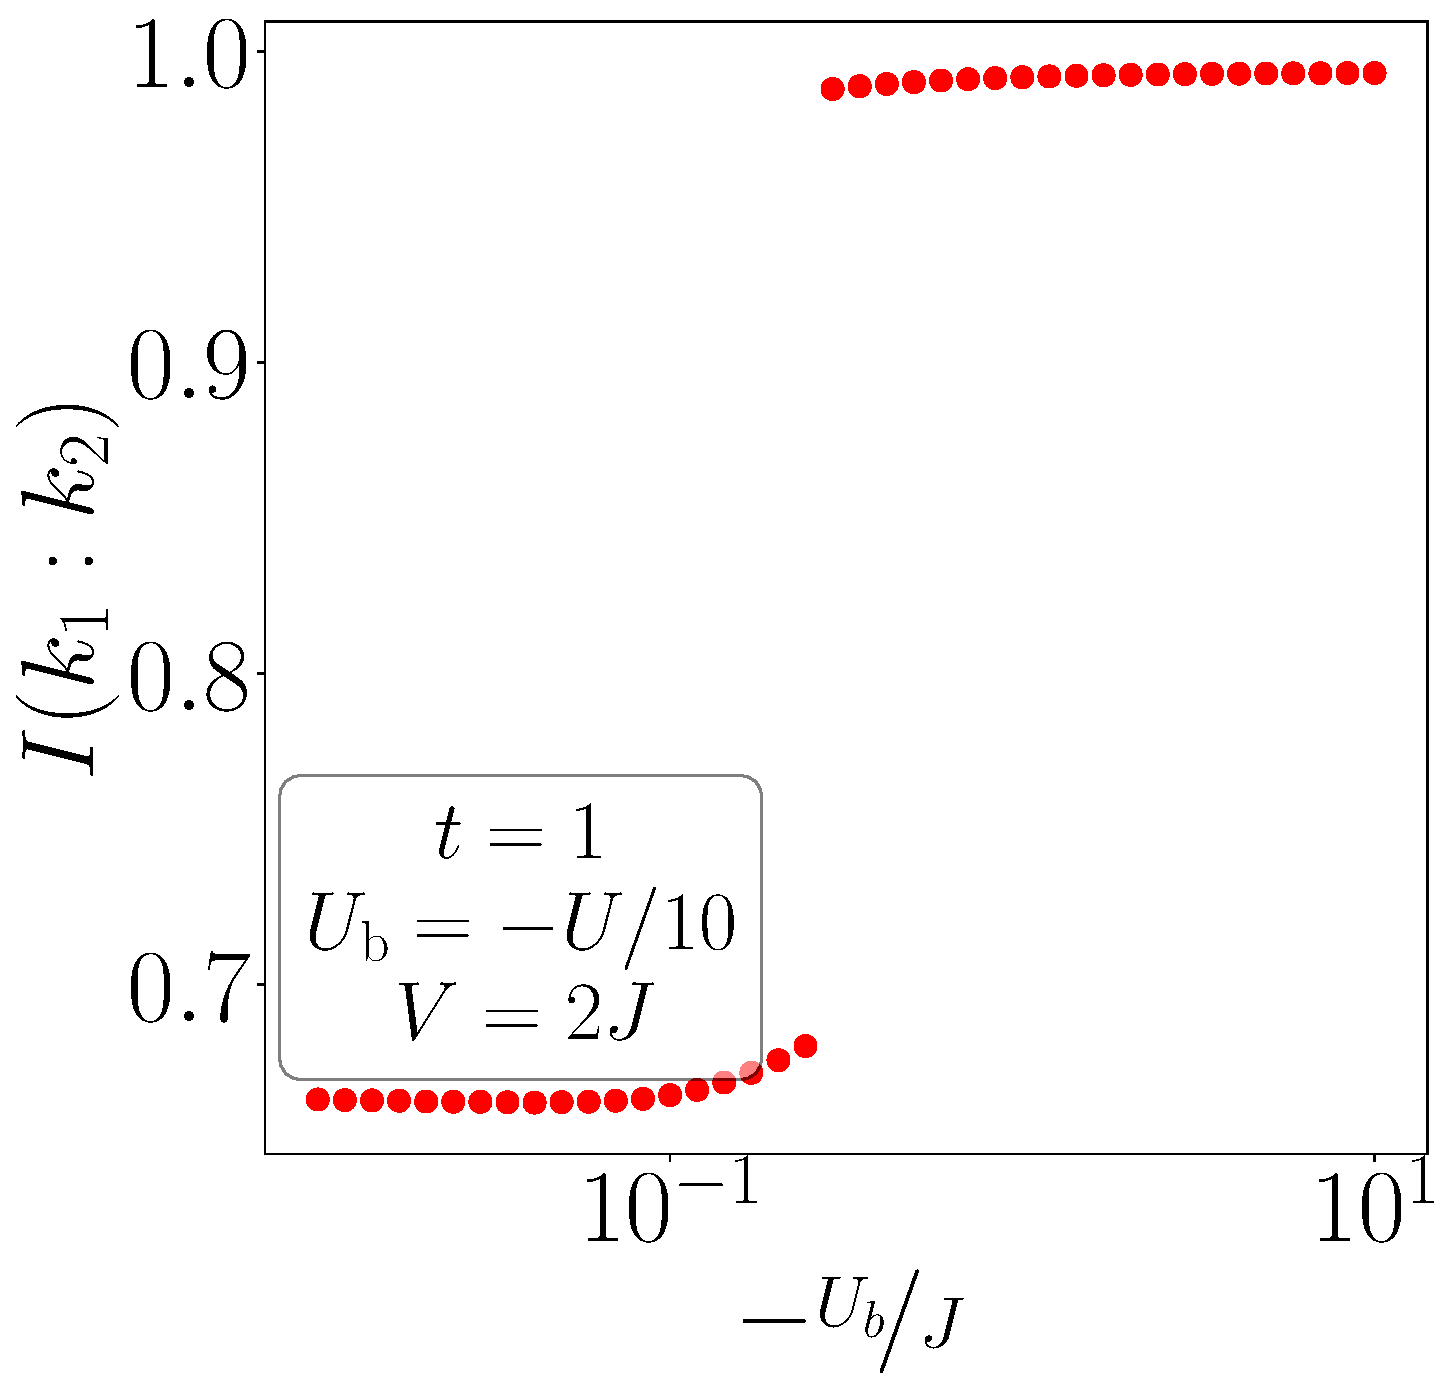
\includegraphics[width=0.49\textwidth]{./figures/corr-k-t=1.000,J=10.000,0.000,40,V=3J,Ubath=-U_by_10,N=4,U=1.000,1000.000,40.pdf}
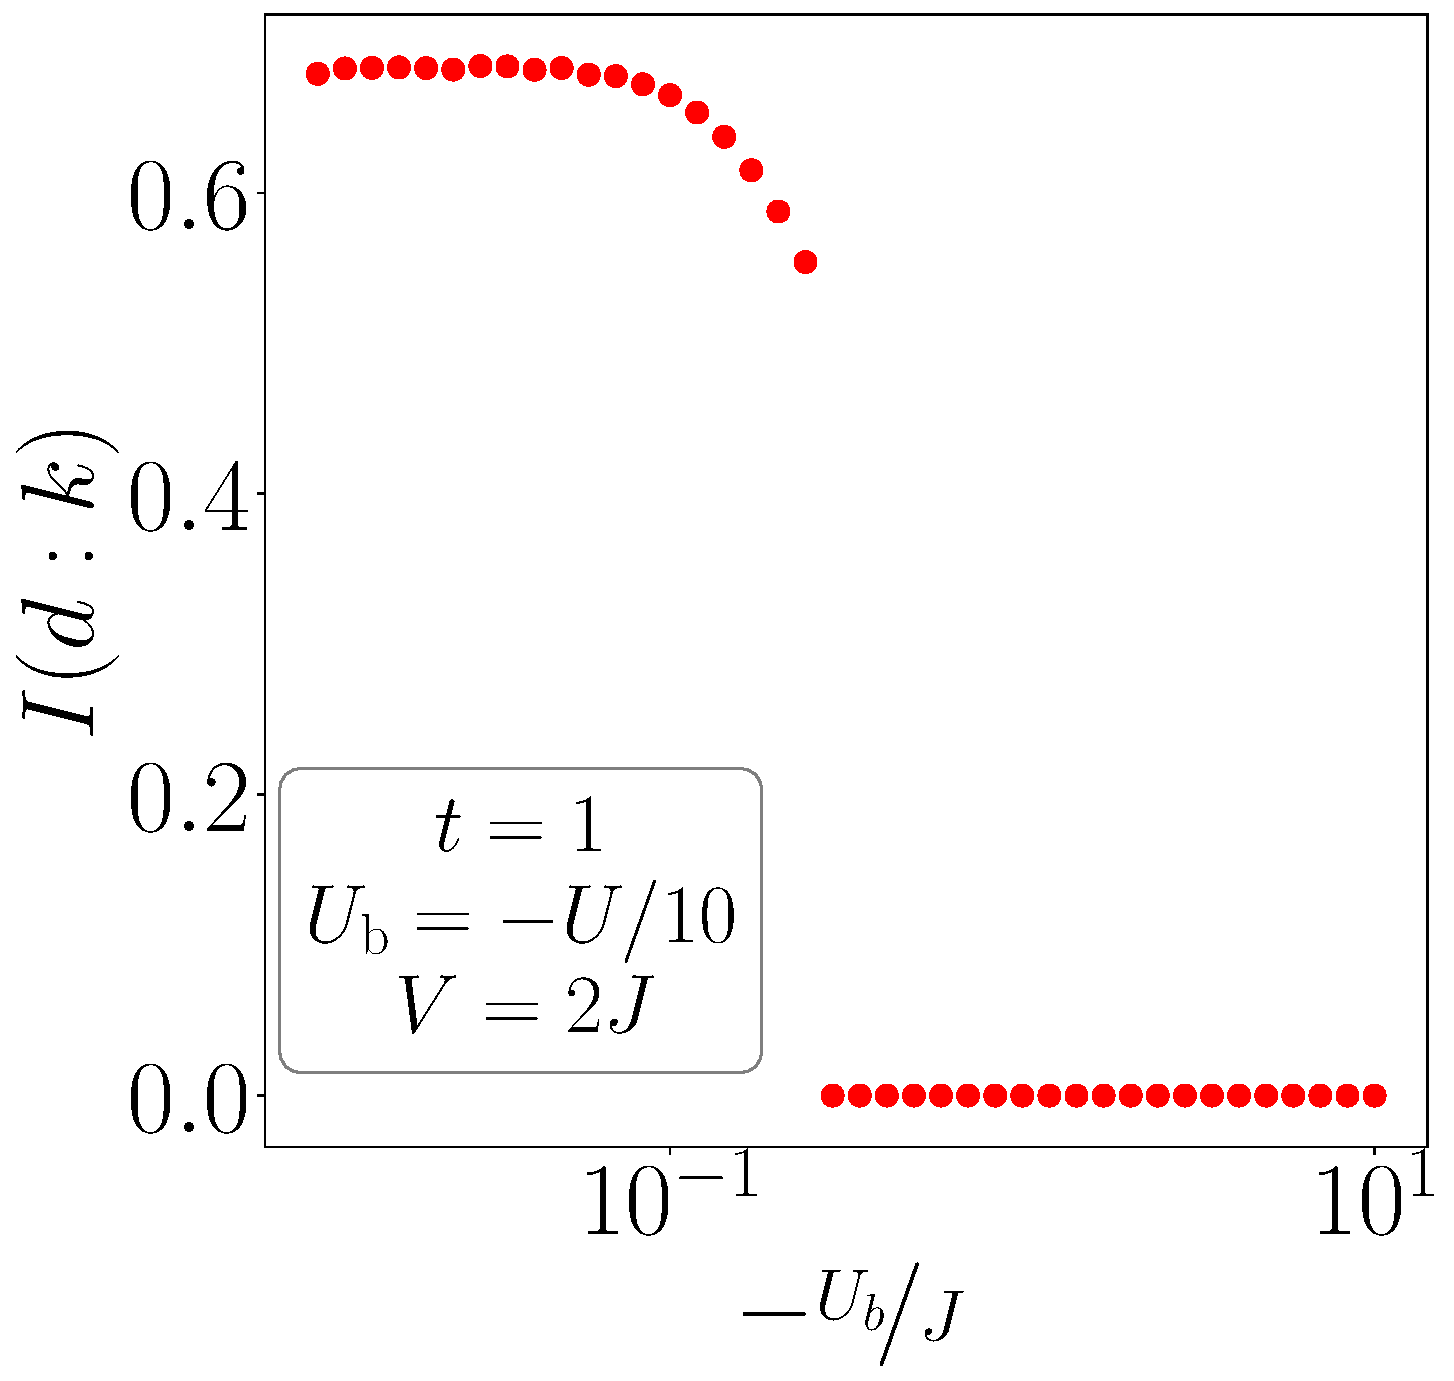
\includegraphics[width=0.49\textwidth]{./figures/mi-dk-t=1.000,J=10.000,0.000,40,V=3J,Ubath=-U_by_10,N=4,U=1.000,1000.000,40.pdf}
\end{frame}

\begin{frame}[noframenumbering]{Correlation measures: Real space mutual information}
\vspace*{20pt}
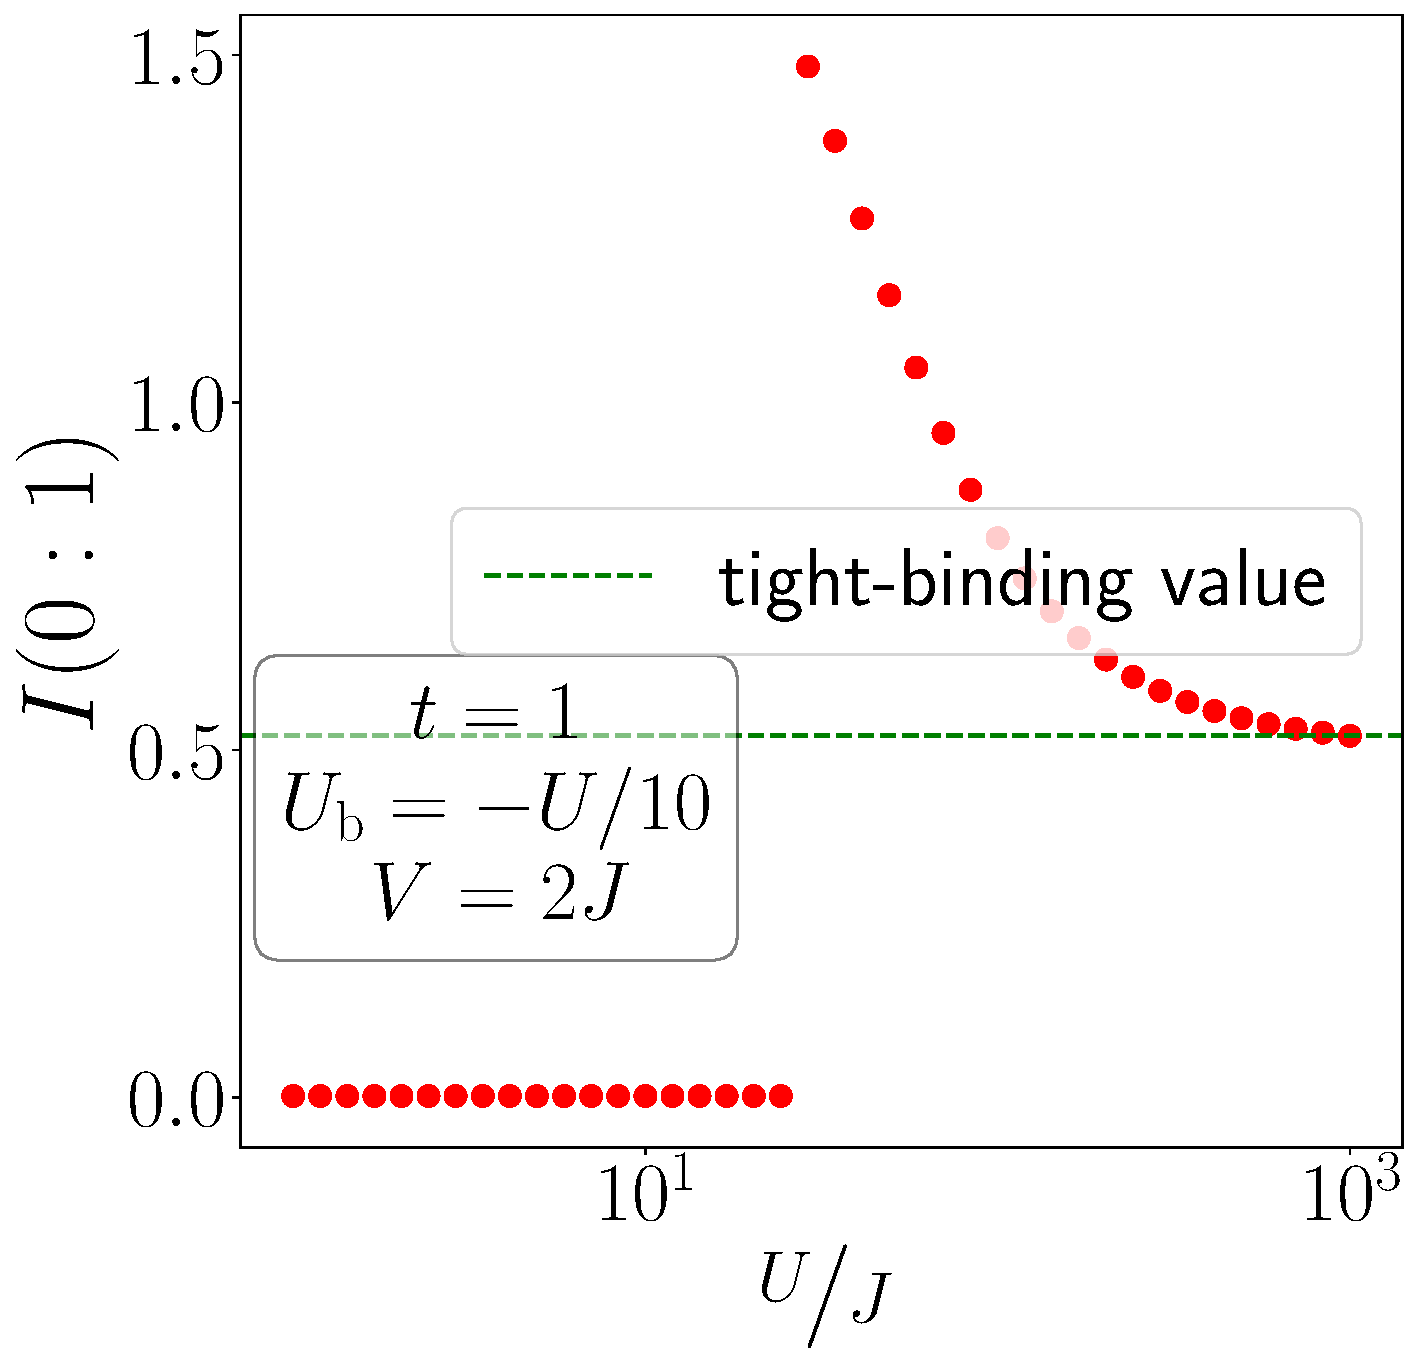
\includegraphics[width=0.49\textwidth]{./figures/mi-01-t=1.000,J=10.000,0.000,40,V=3J,Ubath=-U_by_10,N=4,U=1.000,1000.000,40.pdf}
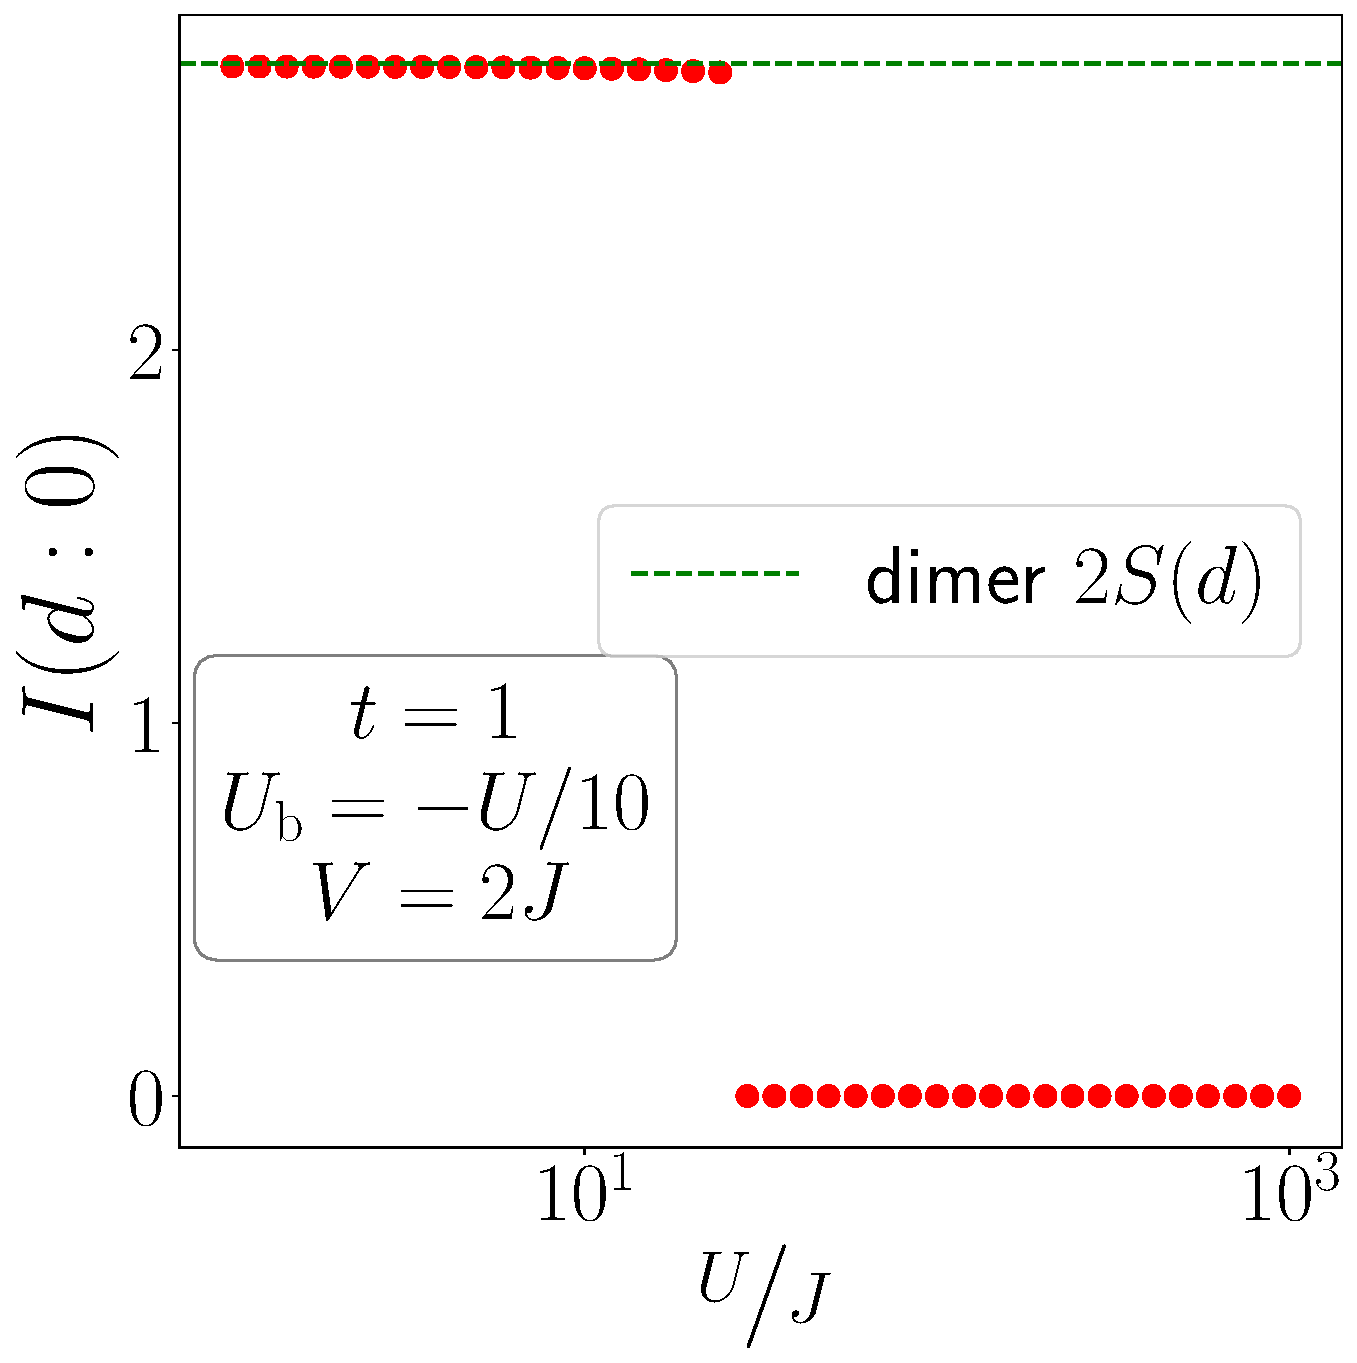
\includegraphics[width=0.49\textwidth]{./figures/mi-d0-t=1.000,J=10.000,0.000,40,V=3J,Ubath=-U_by_10,N=4,U=1.000,1000.000,40.pdf}
\end{frame}


\begin{frame}[noframenumbering]{Correlation measures: Impurity entanglement entropy and spin-spin correlations}
\vspace*{20pt}
	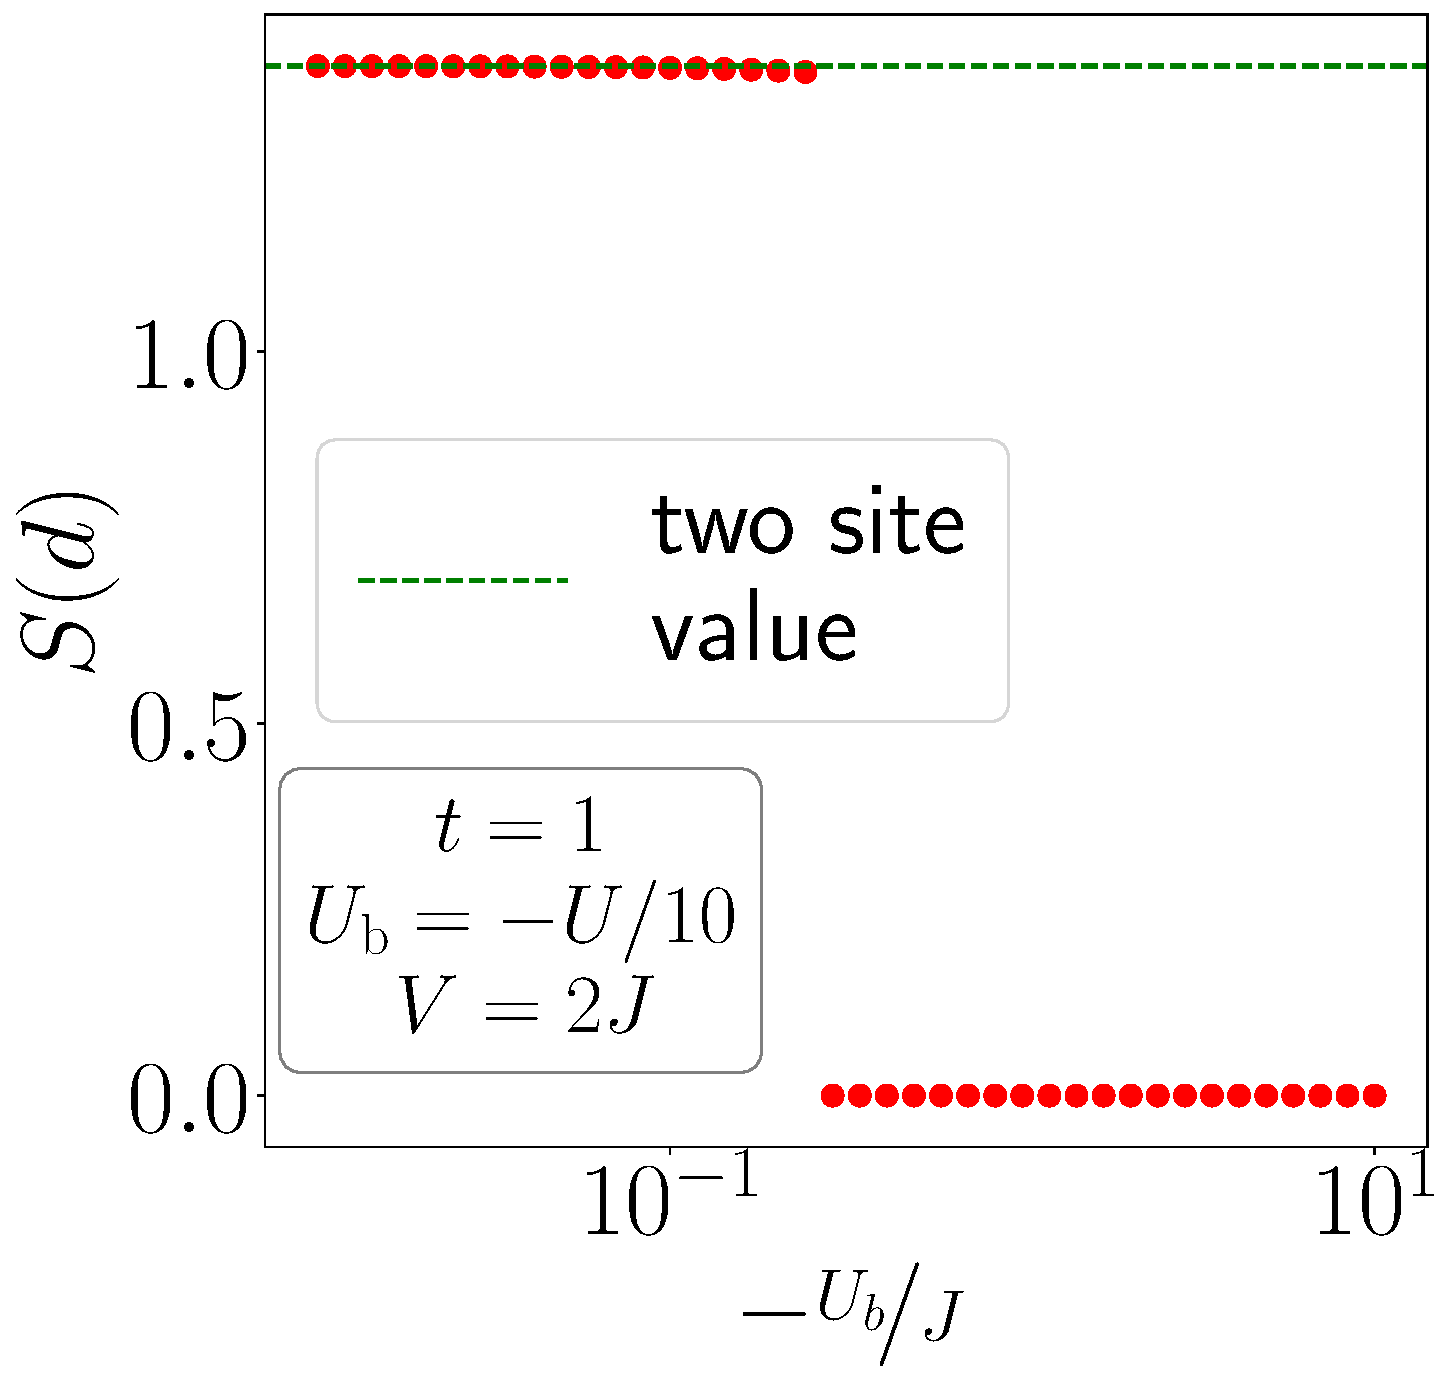
\includegraphics[width=0.32\textwidth]{./figures/EE-d-t=1.000,J=10.000,0.000,40,V=3J,Ubath=-U_by_10,N=4,U=1.000,1000.000,40.pdf}
	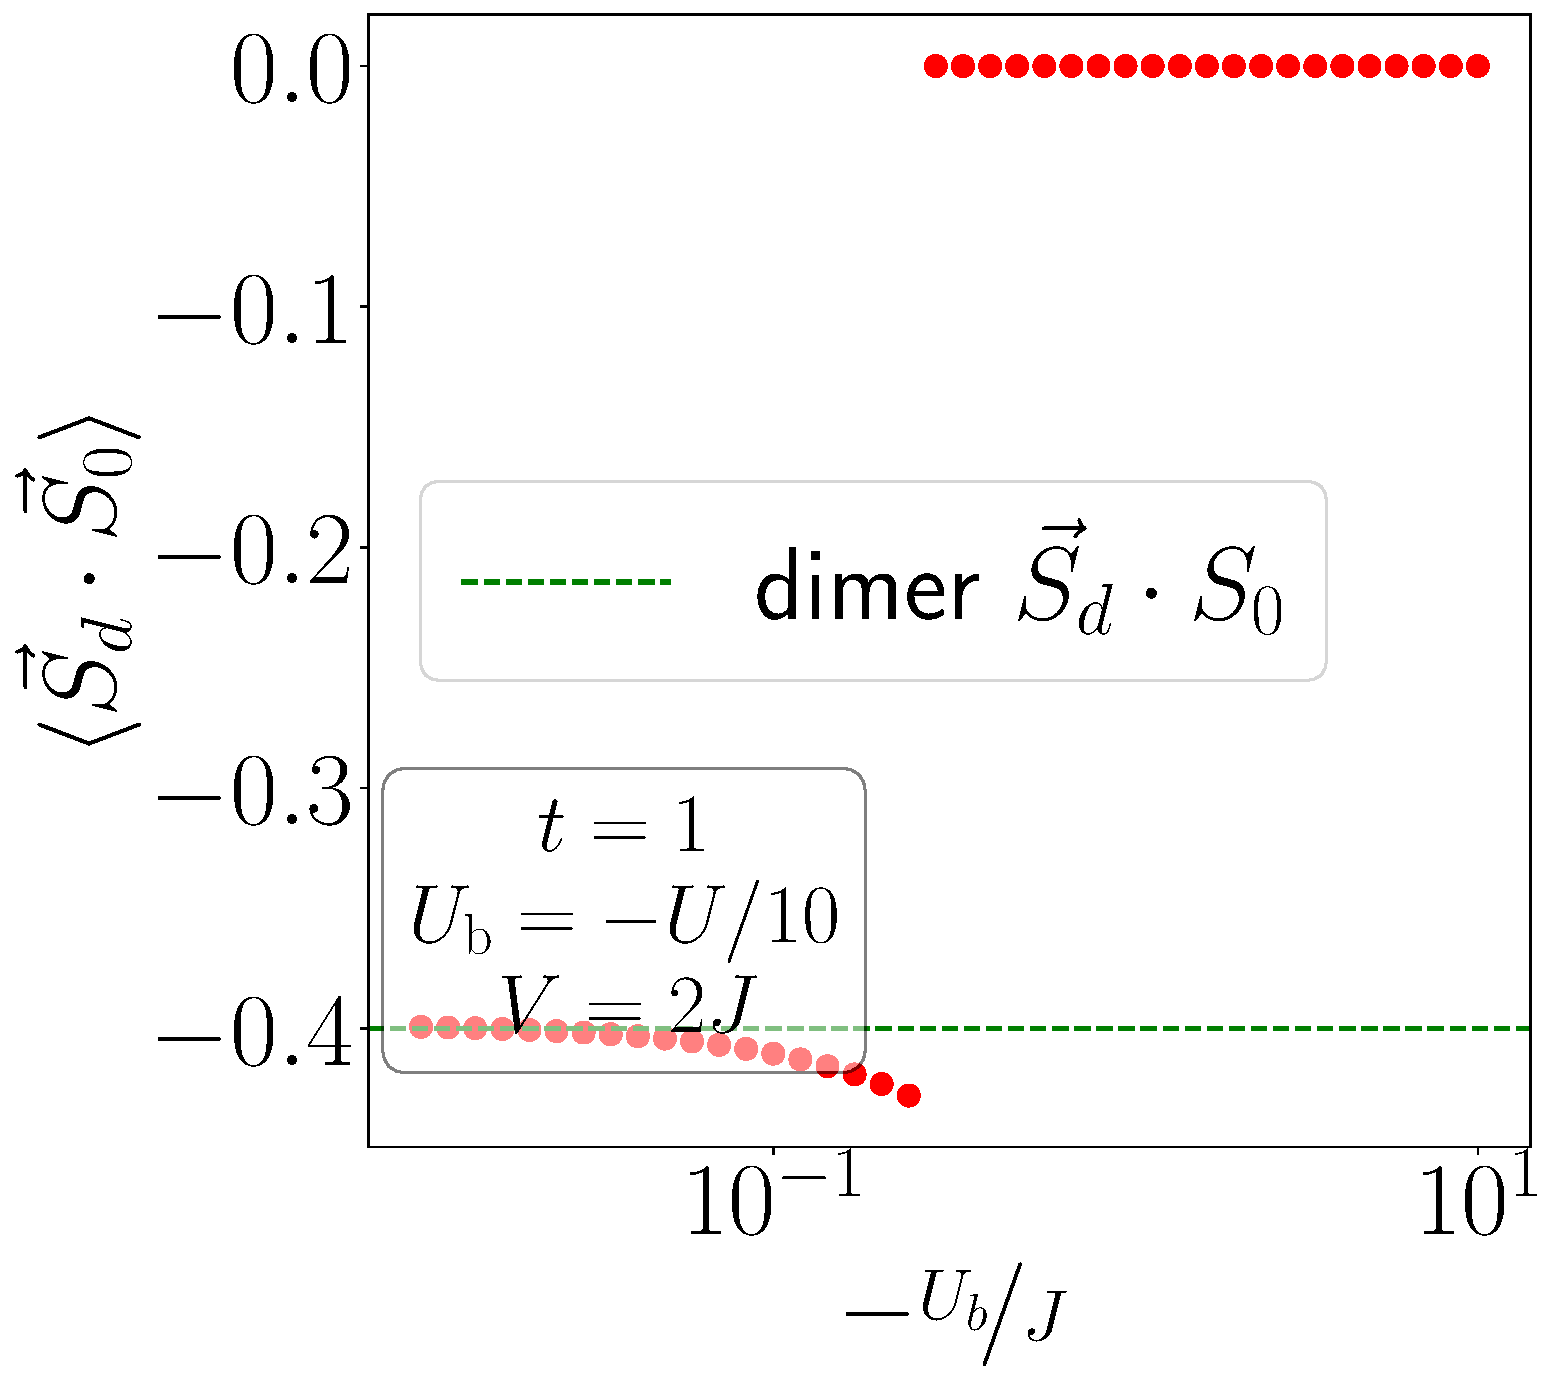
\includegraphics[width=0.32\textwidth]{./figures/corr-d0-t=1.000,J=10.000,0.000,40,V=3J,Ubath=-U_by_10,N=4,U=1.000,1000.000,40.pdf}
	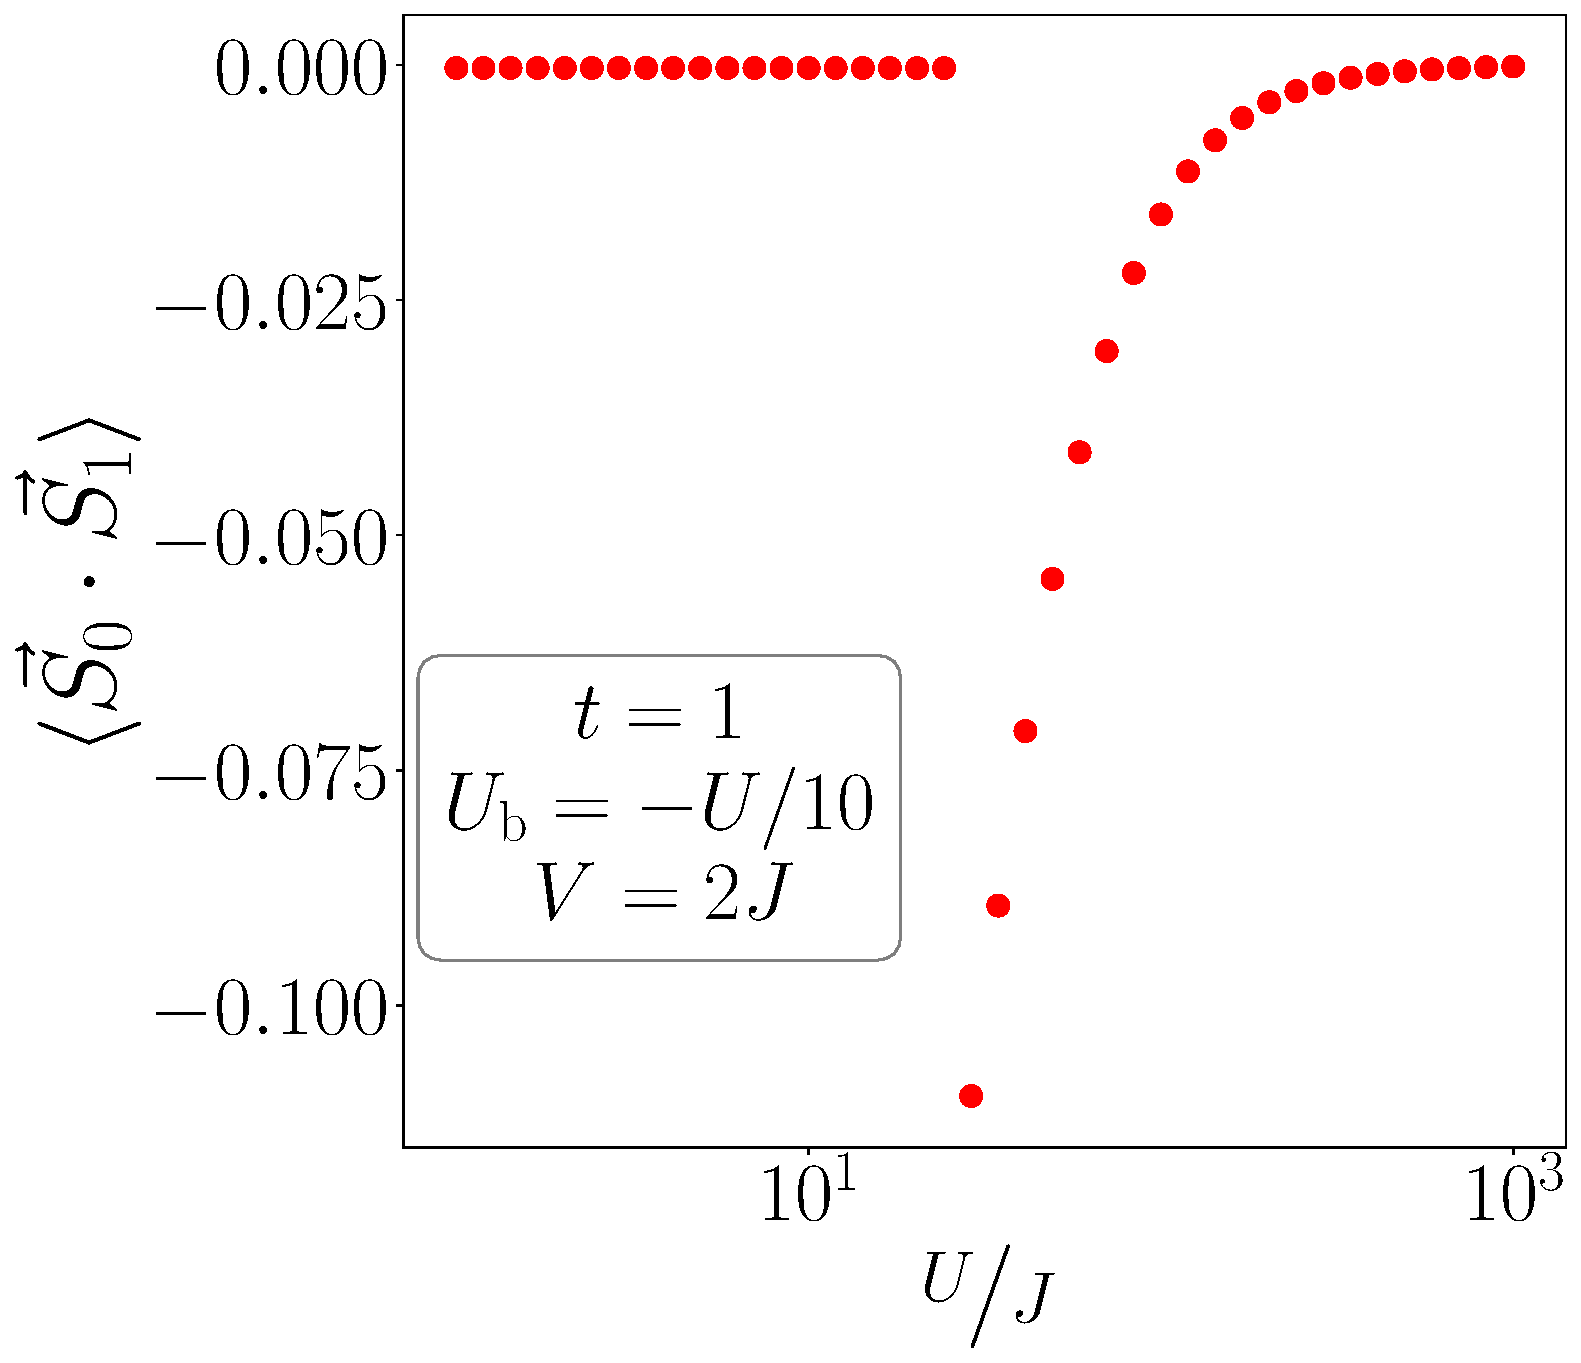
\includegraphics[width=0.32\textwidth]{./figures/r-vec-corr-01-t=1.000,J=10.000,0.000,40,V=3J,Ubath=-U_by_10,N=4,U=1.000,1000.000,40.pdf}
\end{frame}


\begin{frame}[noframenumbering]{Correlation measures: Real-space correlations}
\vspace*{20pt}
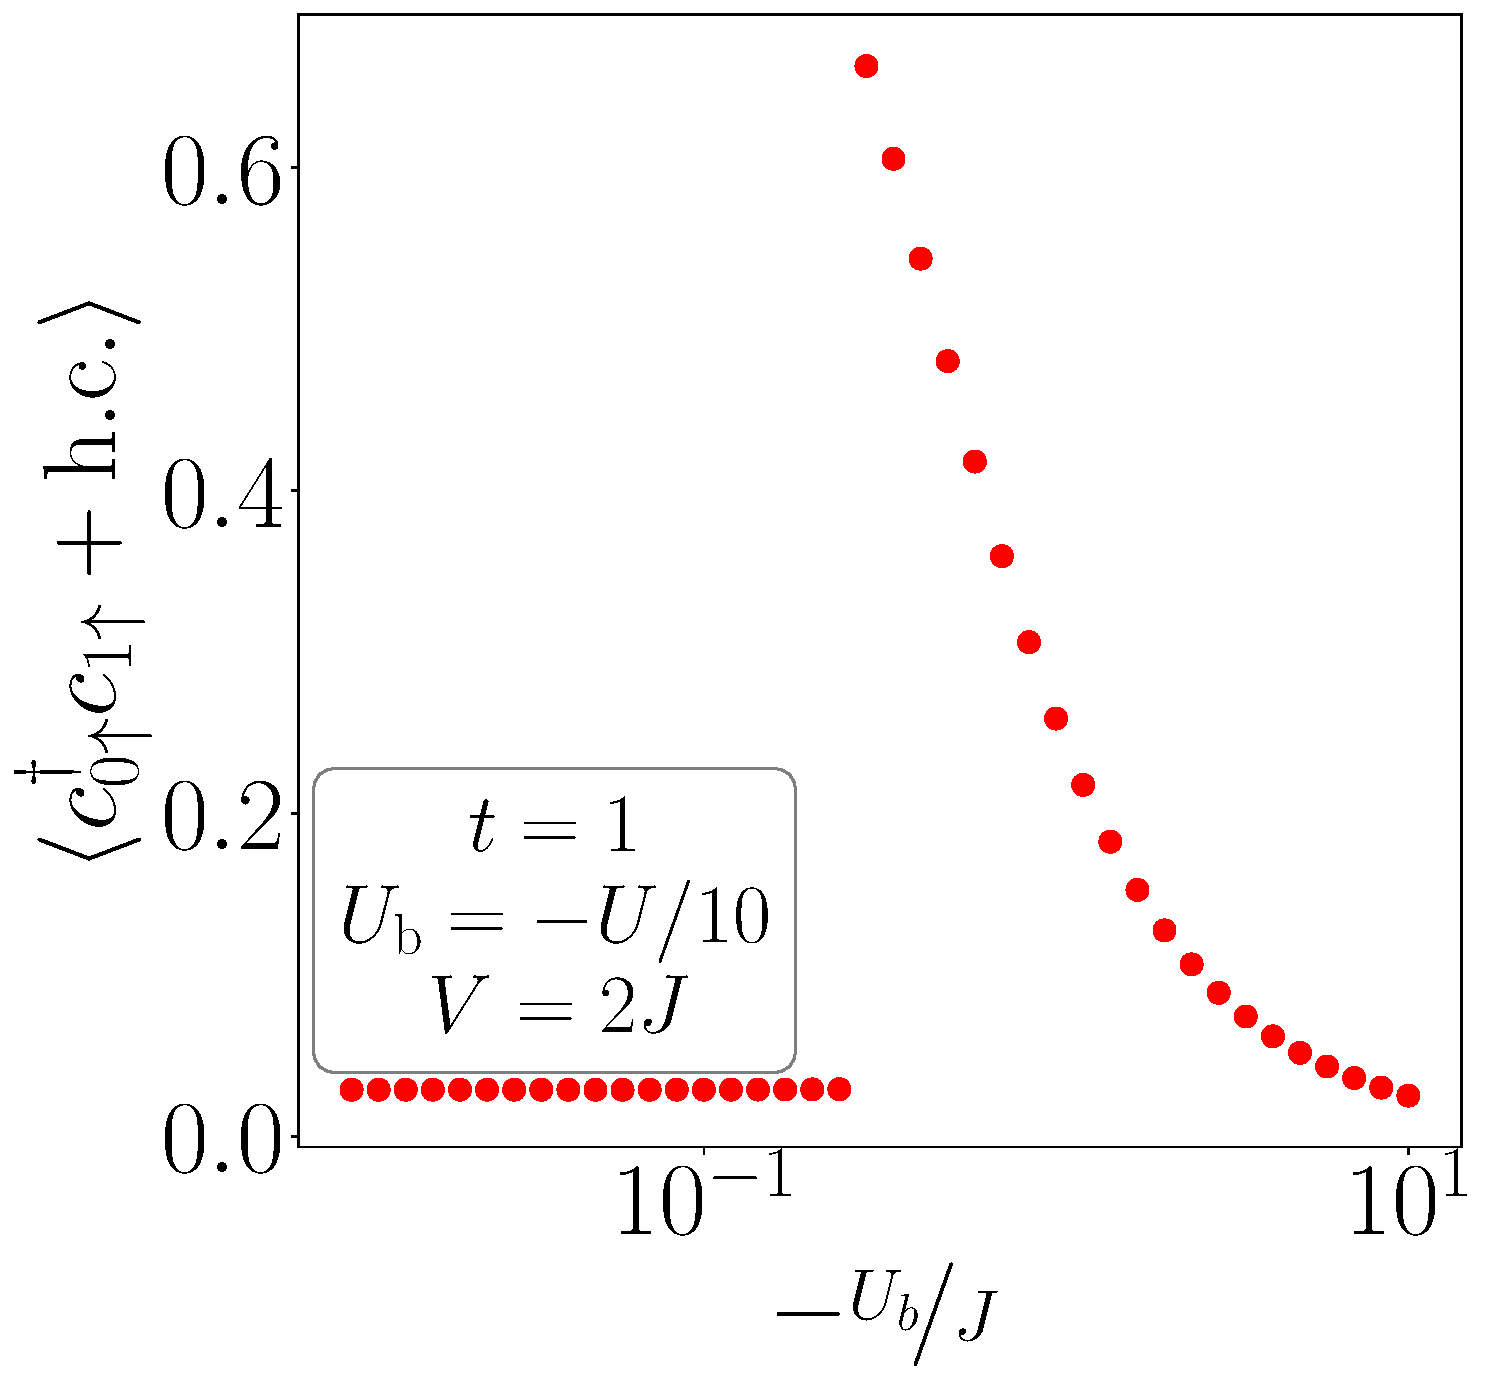
\includegraphics[width=0.49\textwidth]{./figures/r1p-t=1.000,J=10.000,0.000,40,V=3J,Ubath=-U_by_10,N=4,U=1.000,1000.000,40.pdf}
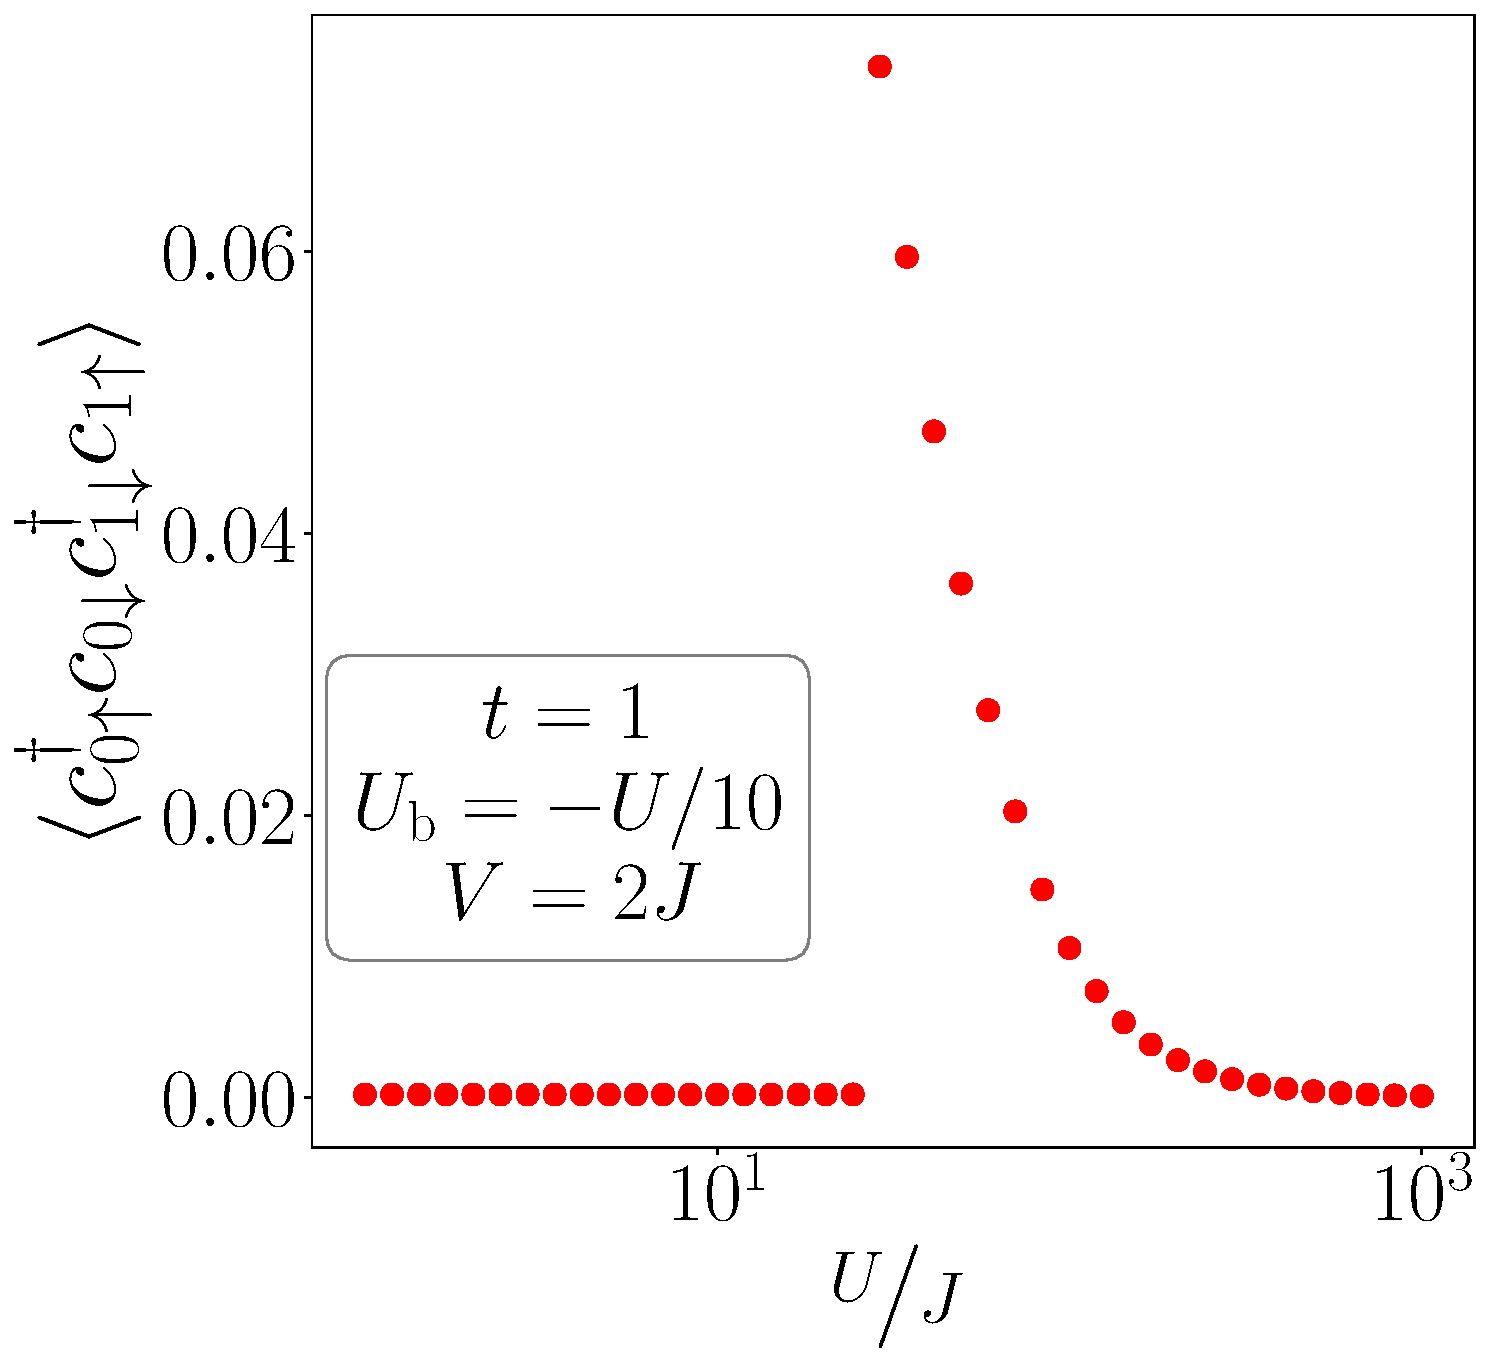
\includegraphics[width=0.49\textwidth]{./figures/r-od-t=1.000,J=10.000,0.000,40,V=3J,Ubath=-U_by_10,N=4,U=1.000,1000.000,40.pdf}
\end{frame}


\begin{frame}[noframenumbering]{Correlation measures: Impurity spectral function}
\centering
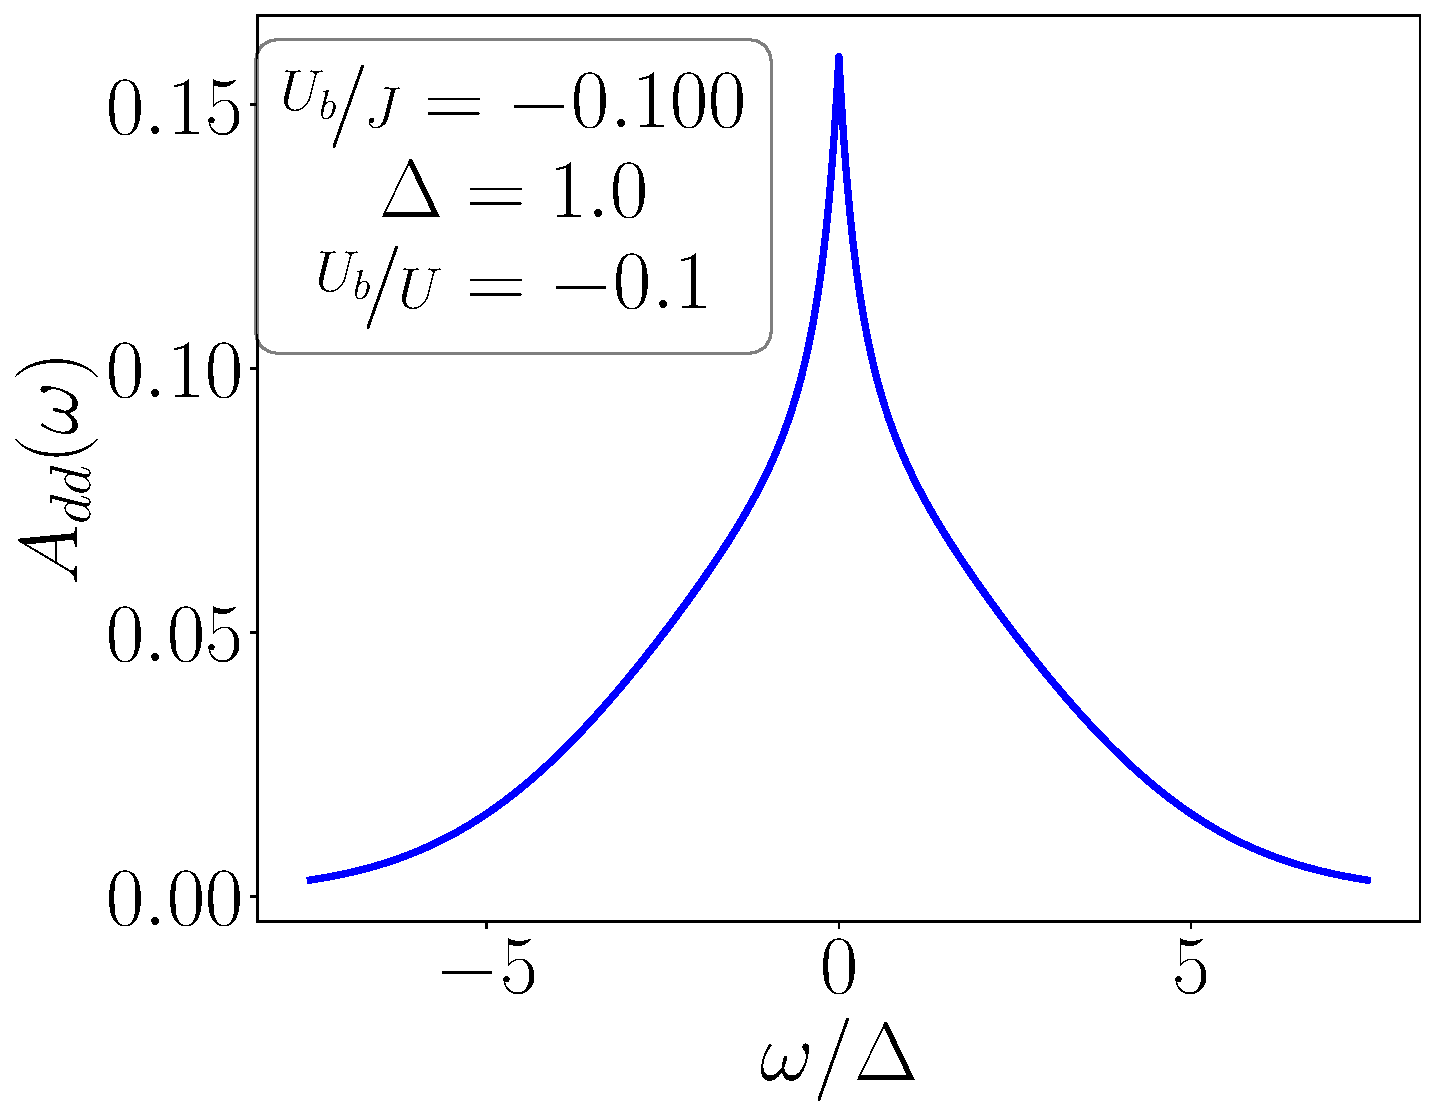
\includegraphics[width=0.32\textwidth]{./figures/spec_func_Ub_by_J=-0.100.pdf}
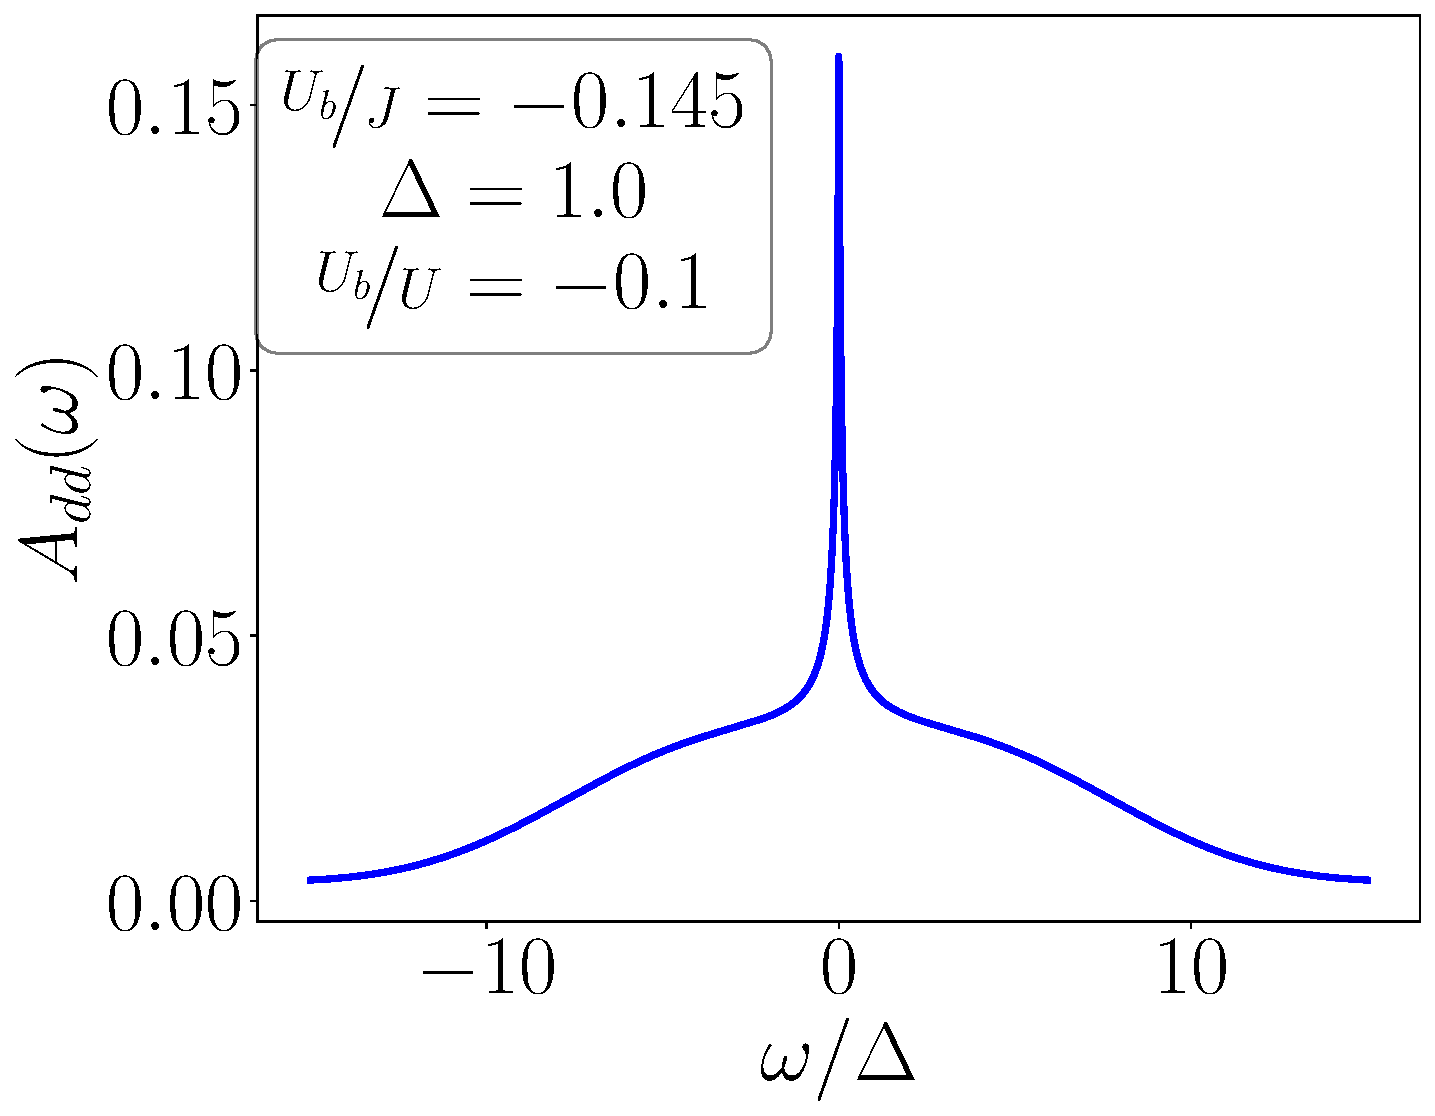
\includegraphics[width=0.32\textwidth]{./figures/spec_func_Ub_by_J=-0.145.pdf}
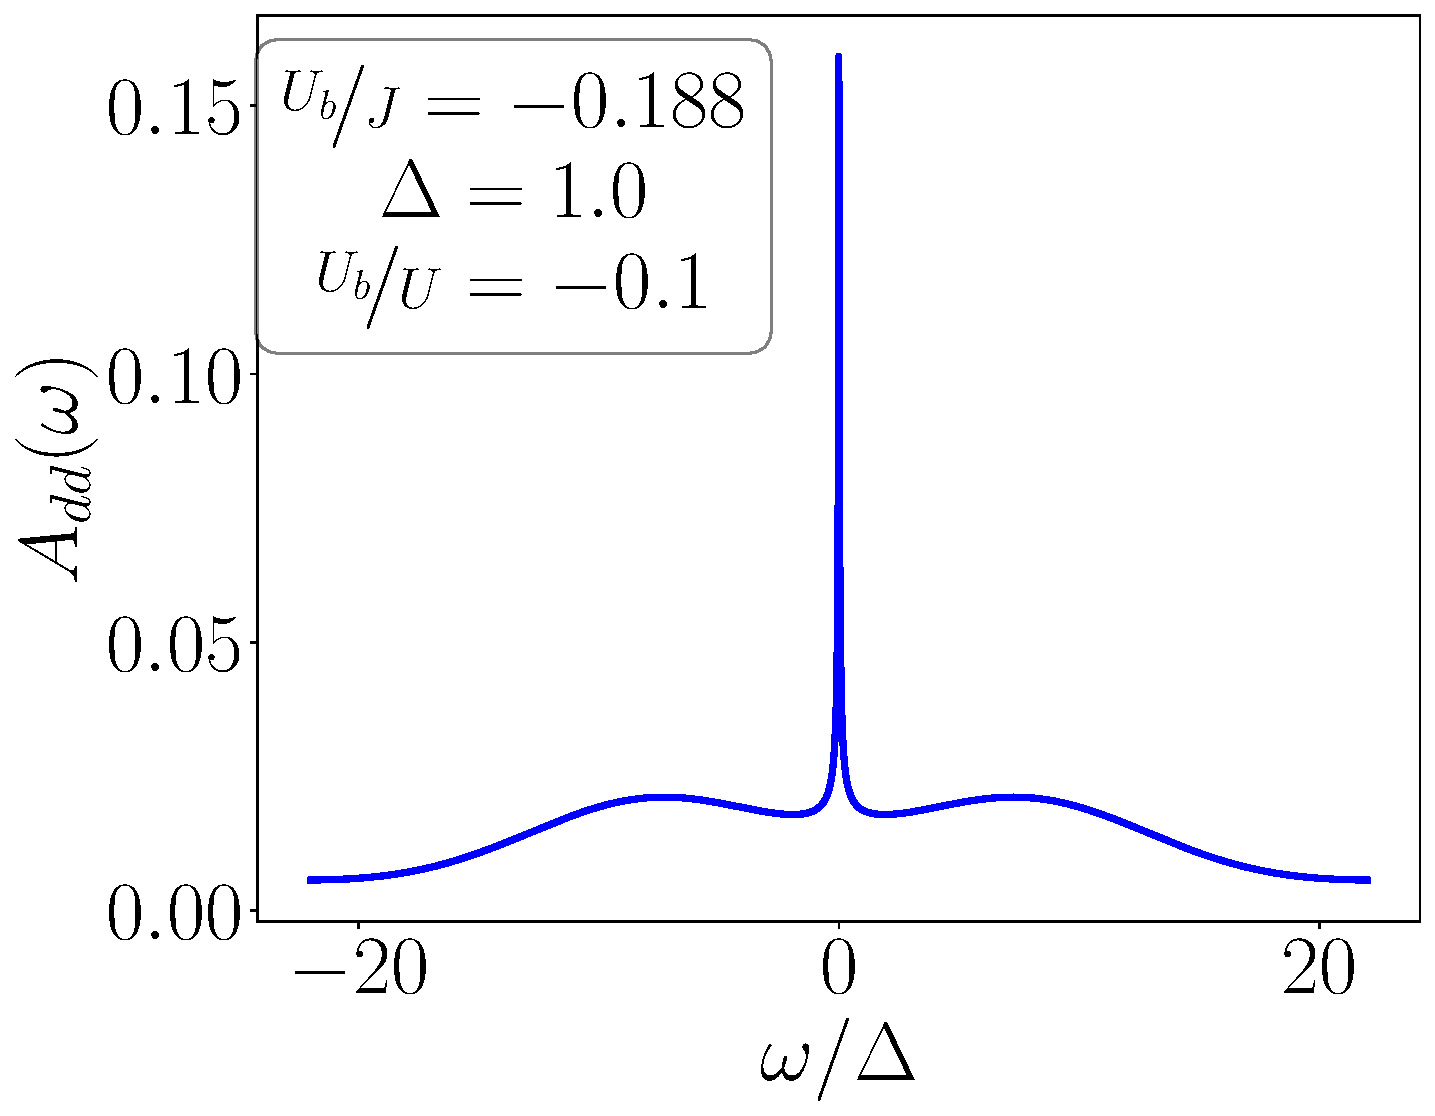
\includegraphics[width=0.32\textwidth]{./figures/spec_func_Ub_by_J=-0.188.pdf}
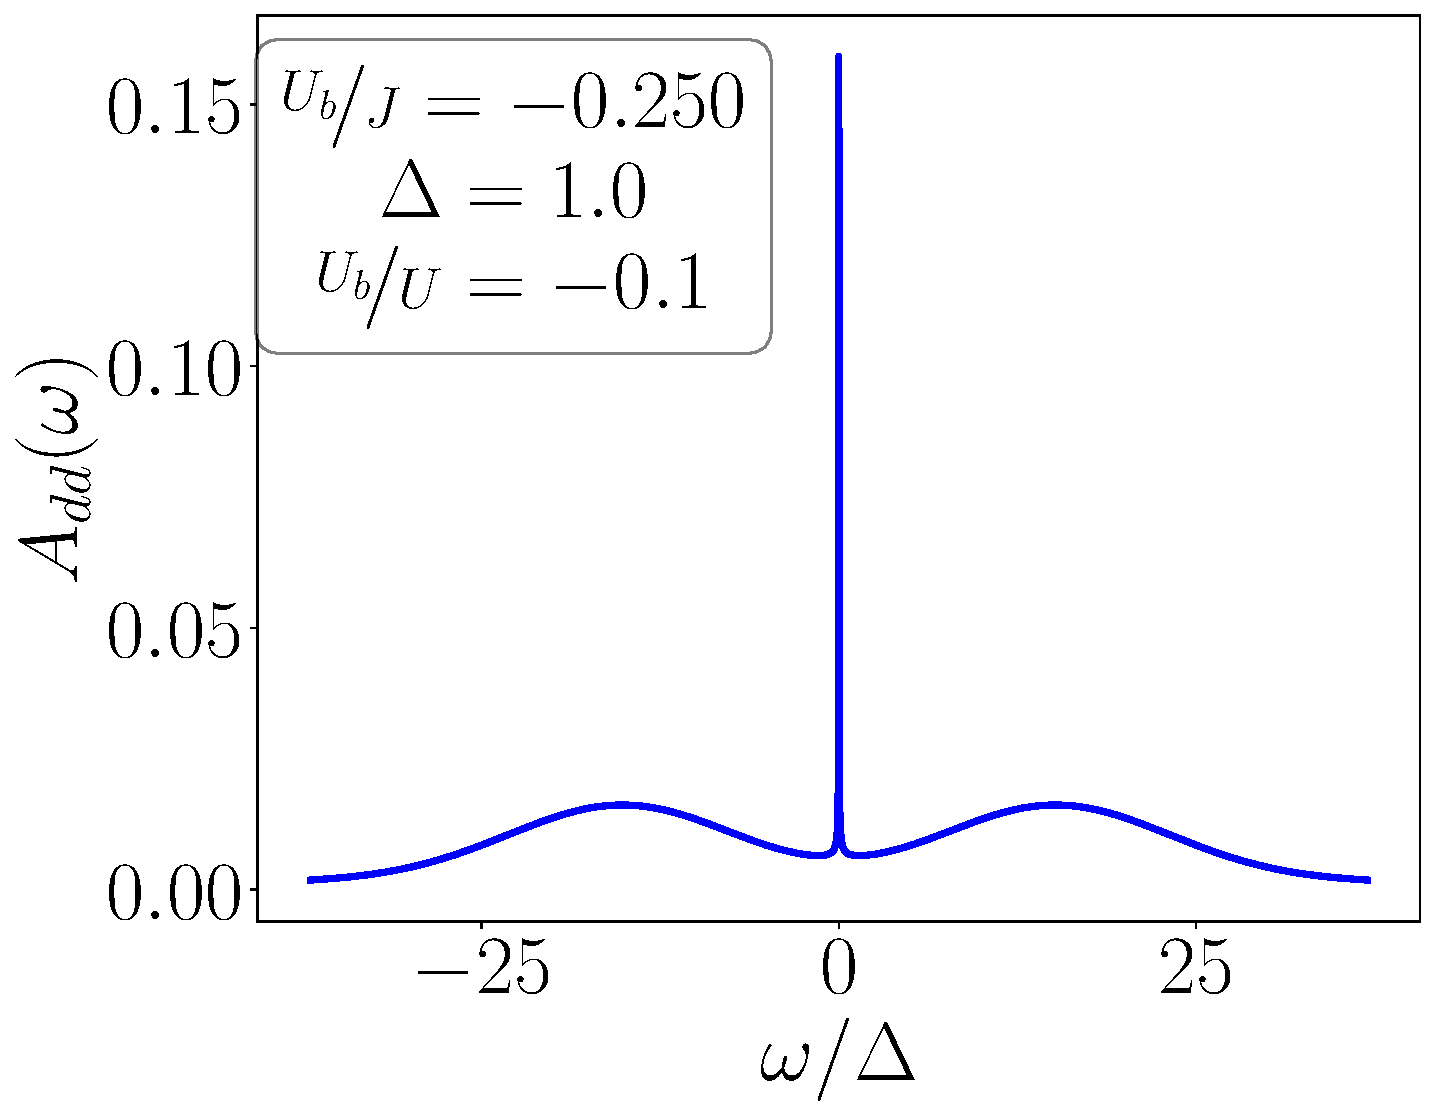
\includegraphics[width=0.32\textwidth]{./figures/spec_func_Ub_by_J=-0.250.pdf}
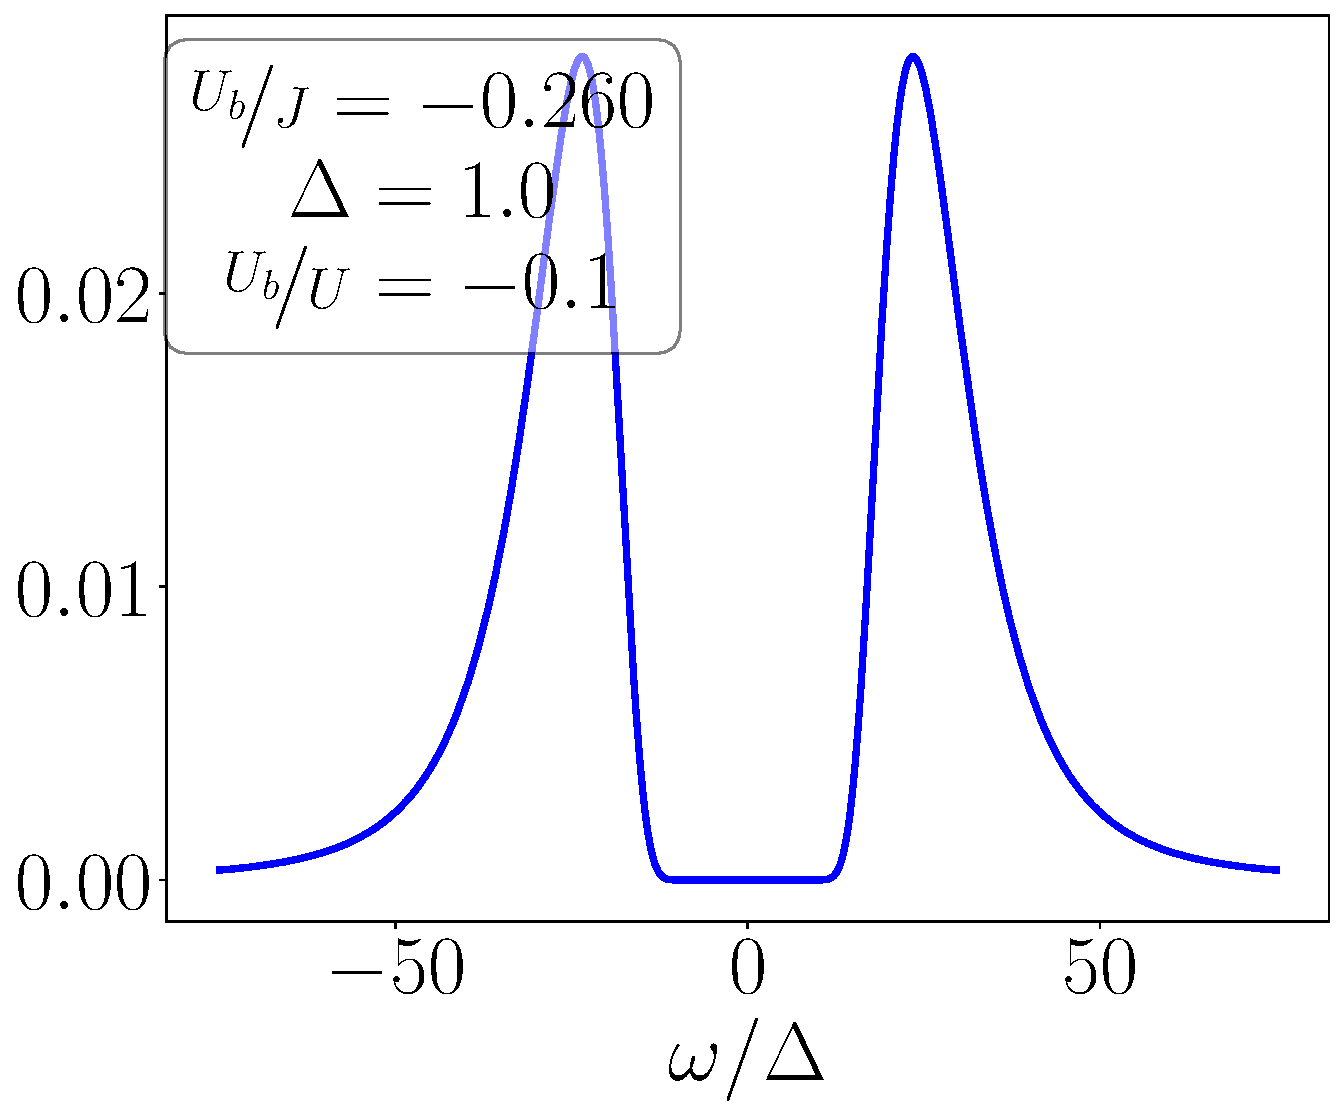
\includegraphics[width=0.32\textwidth]{./figures/spec_func_Ub_by_J=-0.26.pdf}
\end{frame}


\begin{frame}[noframenumbering]{Correlation measures: Impurity-bath spectral function \(A_{d0}\)}
\centering
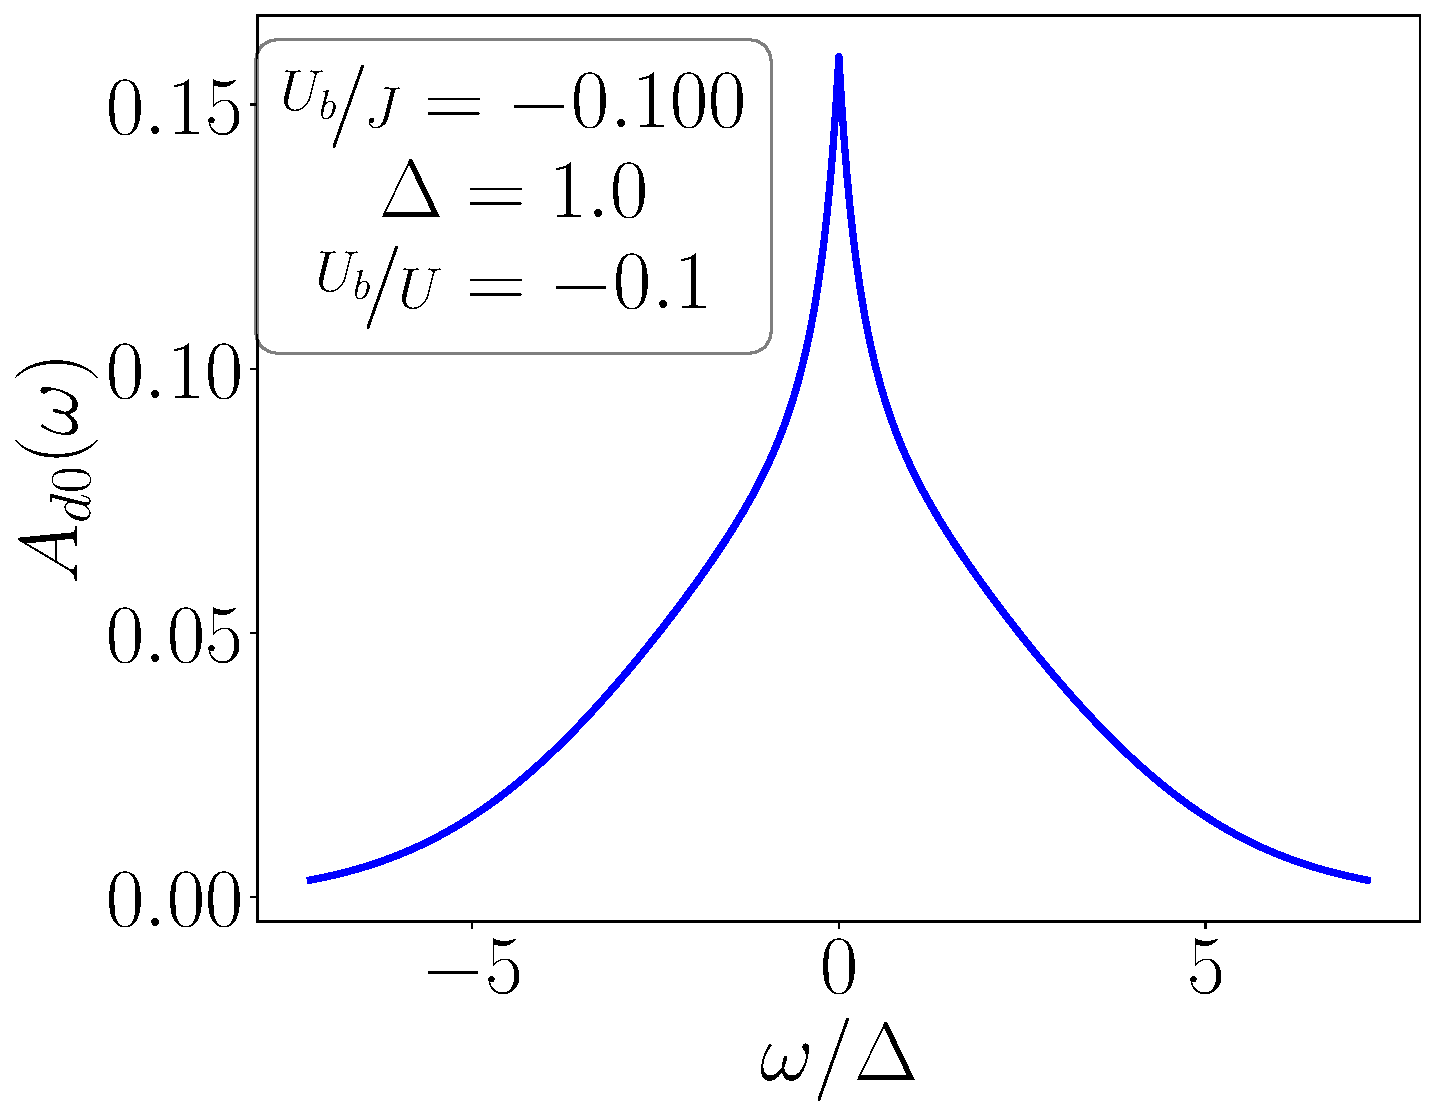
\includegraphics[width=0.32\textwidth]{./figures/spec_func_d0_Ub_by_J=-0.100.pdf}
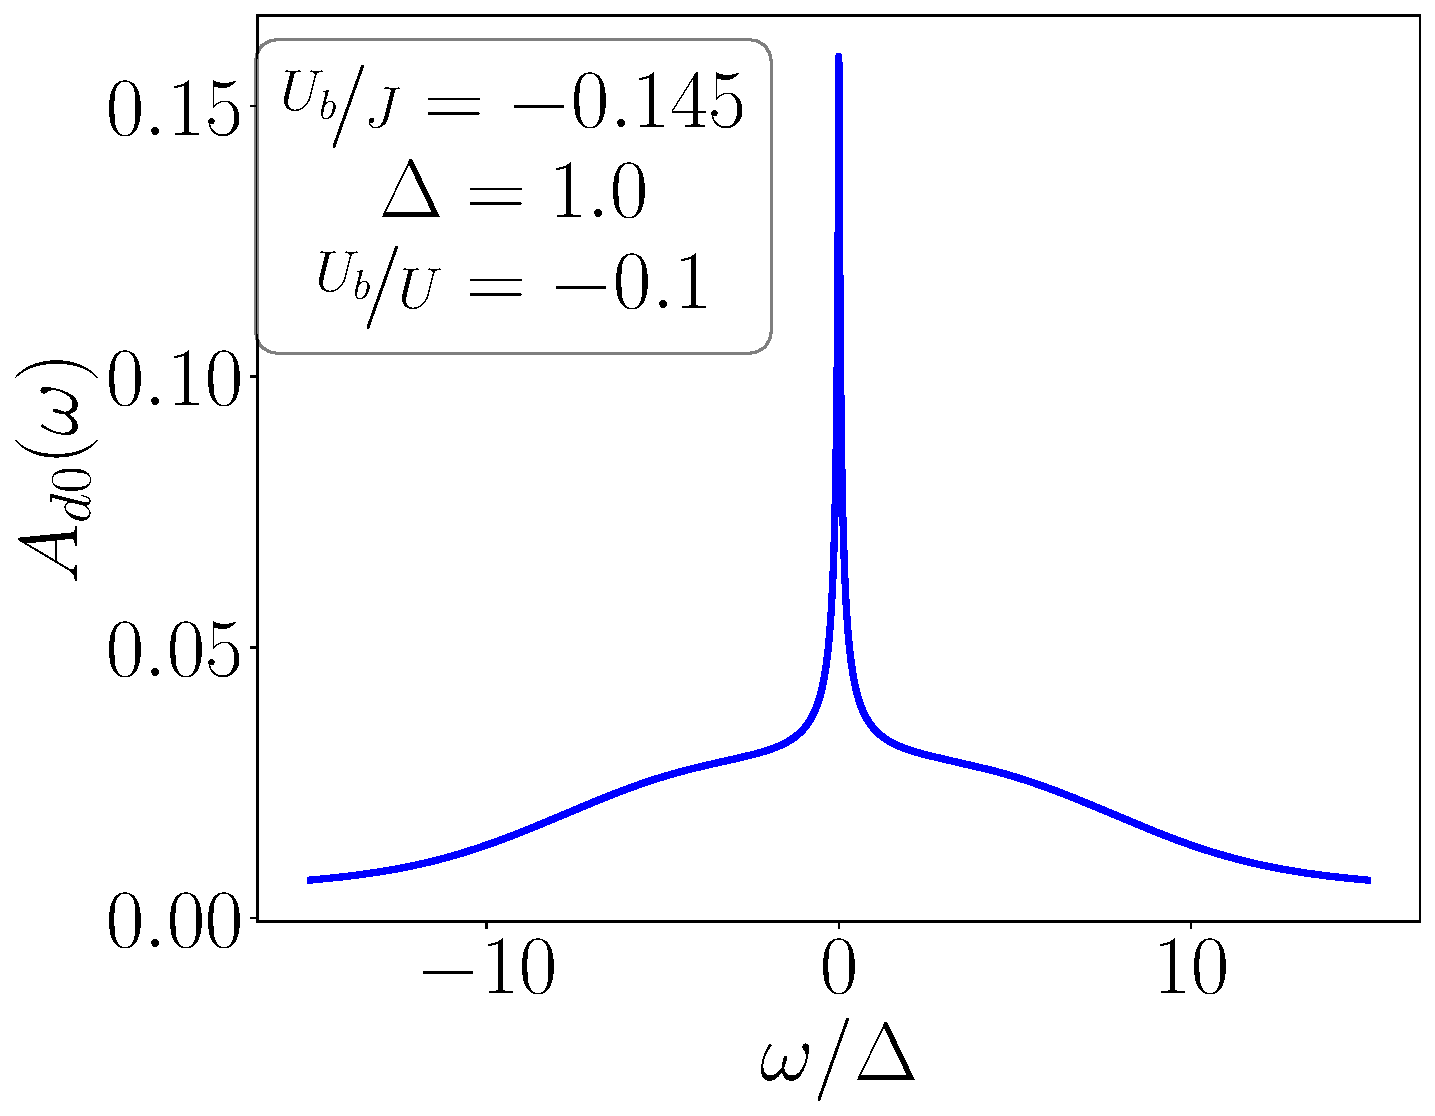
\includegraphics[width=0.32\textwidth]{./figures/spec_func_d0_Ub_by_J=-0.145.pdf}
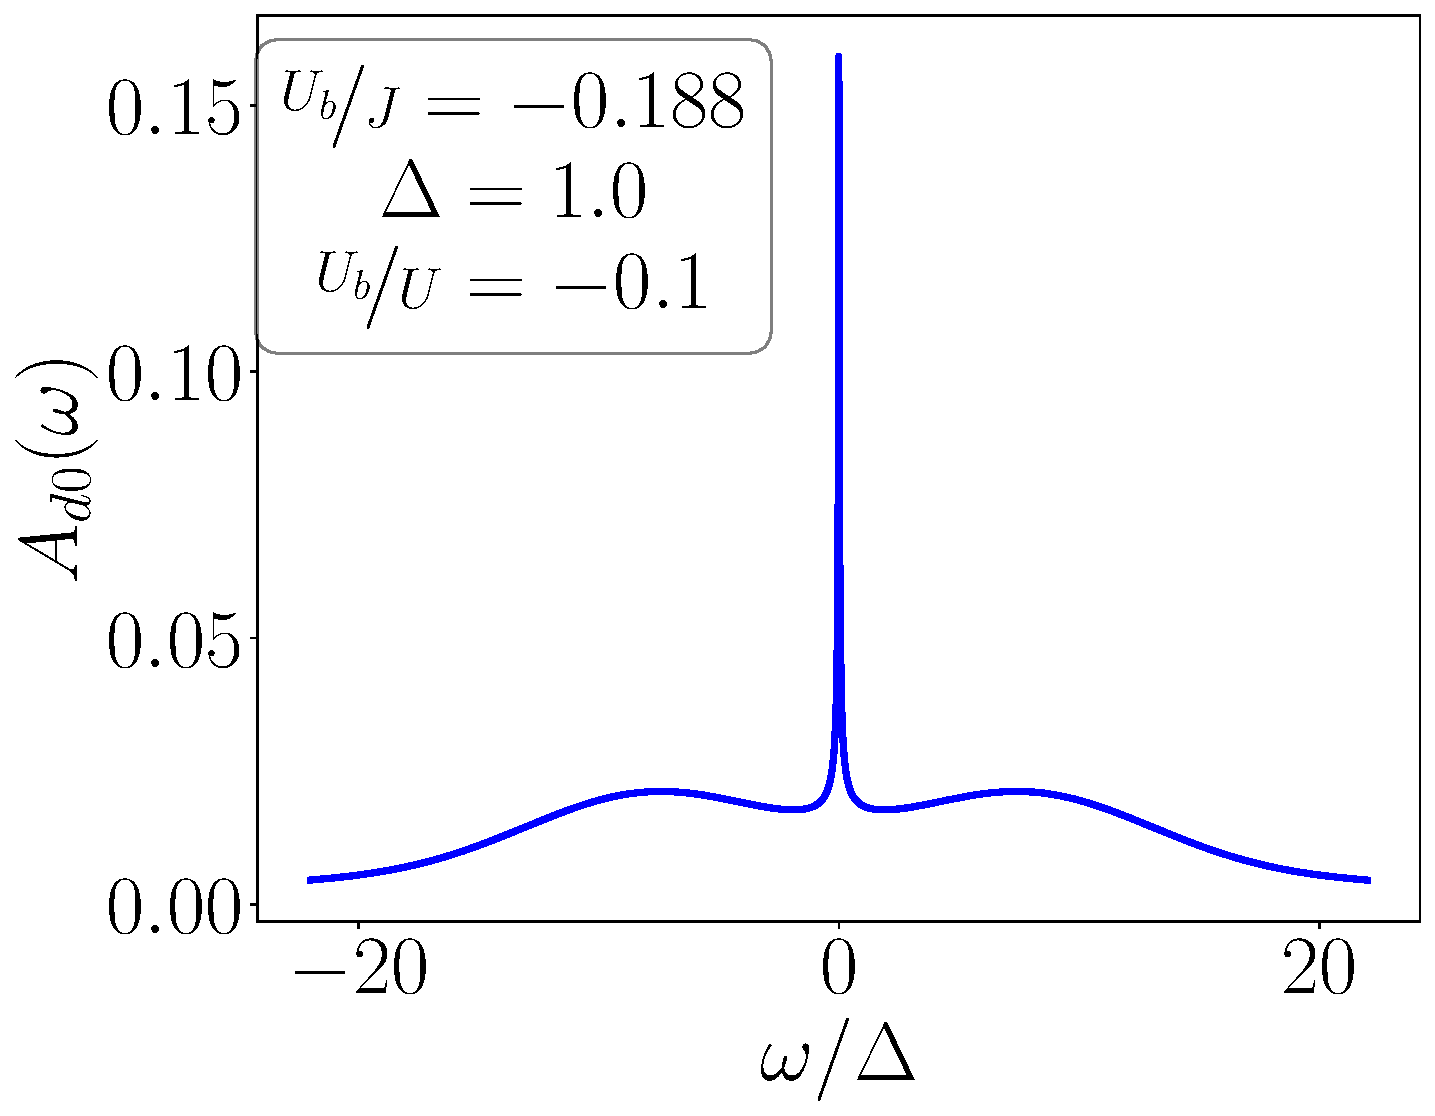
\includegraphics[width=0.32\textwidth]{./figures/spec_func_d0_Ub_by_J=-0.188.pdf}
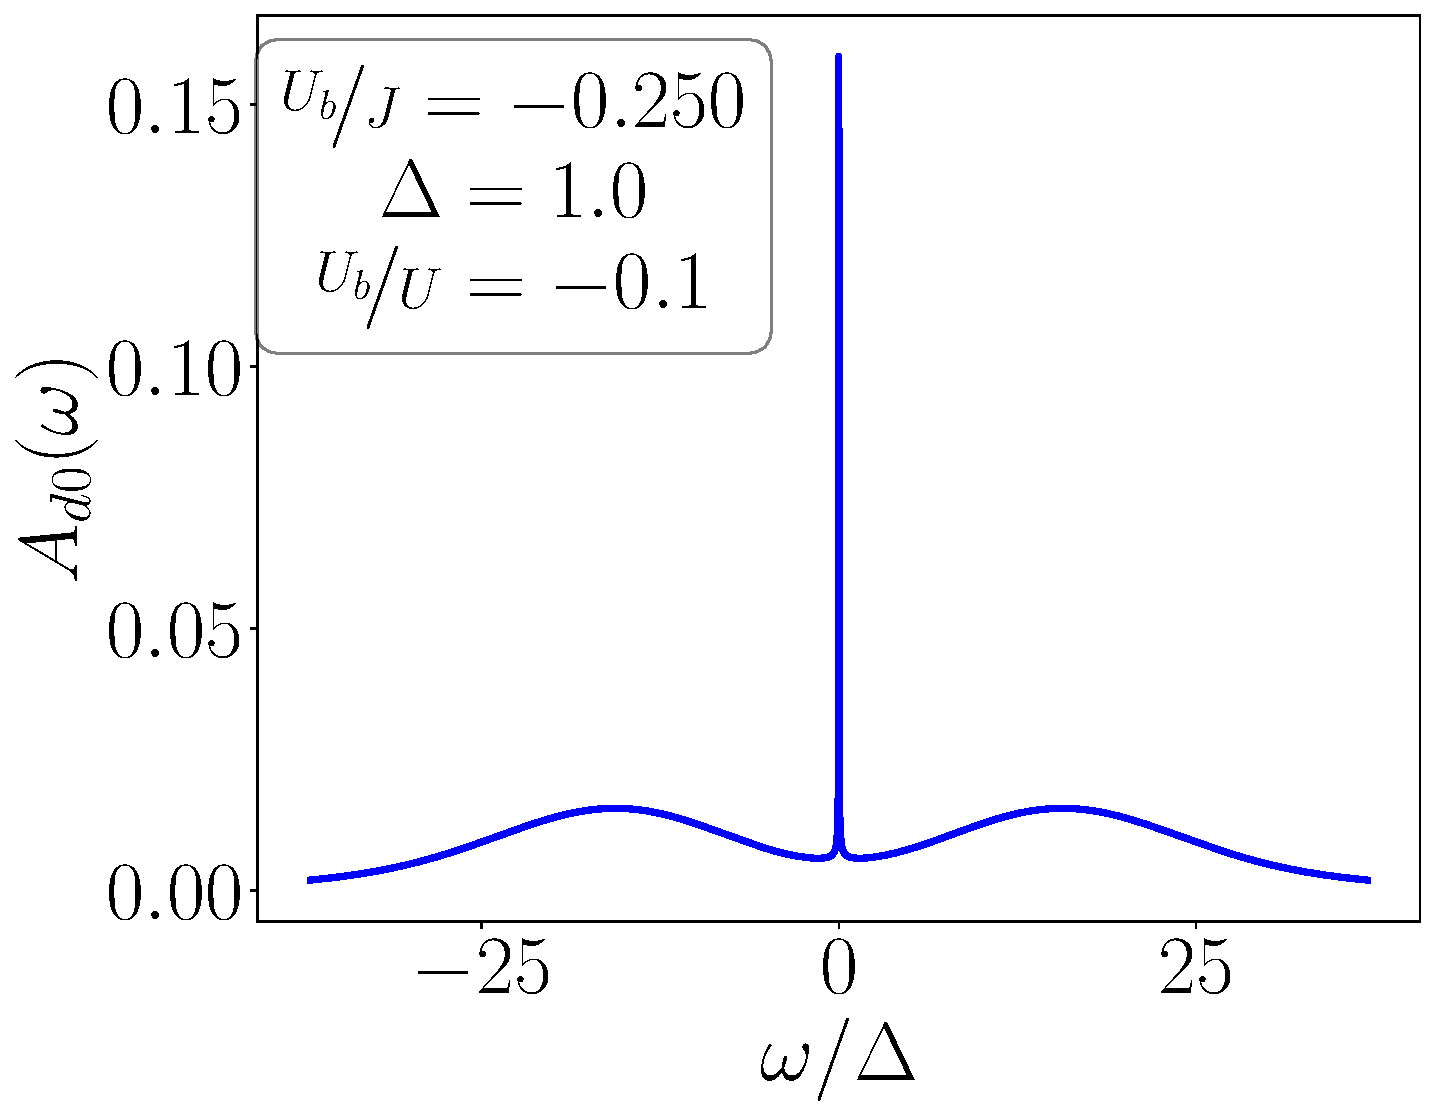
\includegraphics[width=0.32\textwidth]{./figures/spec_func_d0_Ub_by_J=-0.250.pdf}
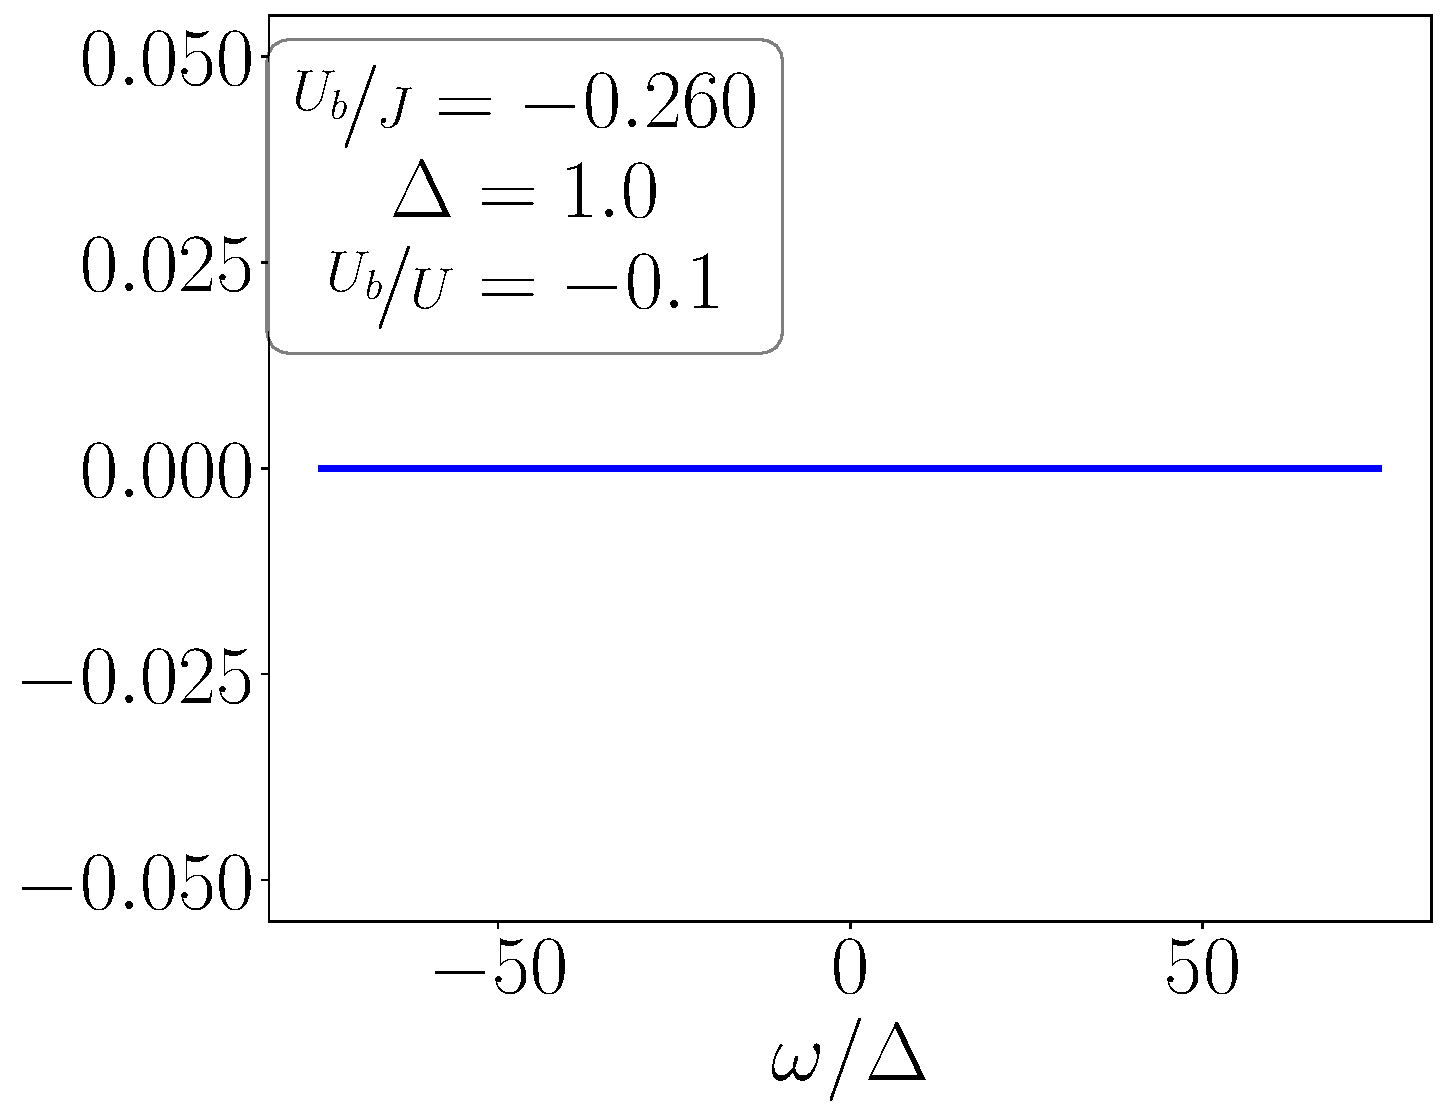
\includegraphics[width=0.32\textwidth]{./figures/spec_func_d0_Ub_by_J=-0.26.pdf}
\end{frame}


\begin{frame}[noframenumbering]{Correlation measures: Bath spectral function \(A_{00}\)}
\centering
\hspace*{\fill}
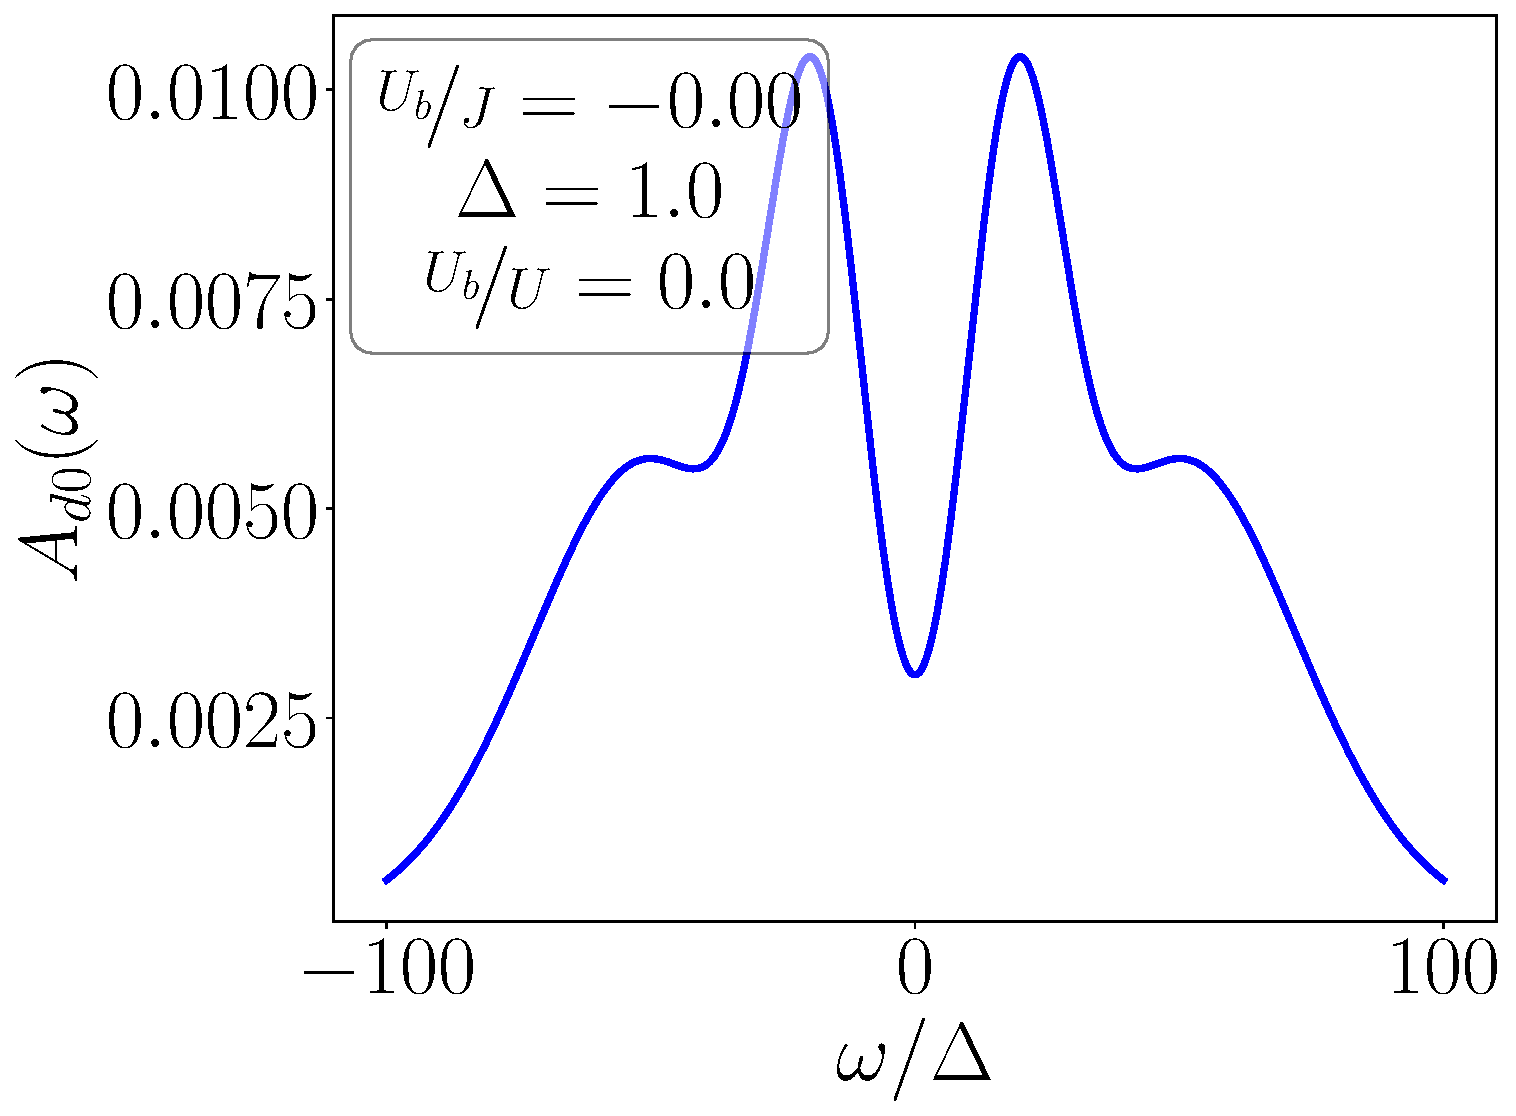
\includegraphics[width=0.33\textwidth]{./figures/spec_func_00_Ub_by_J=-0.000.pdf}
\hspace*{\fill}
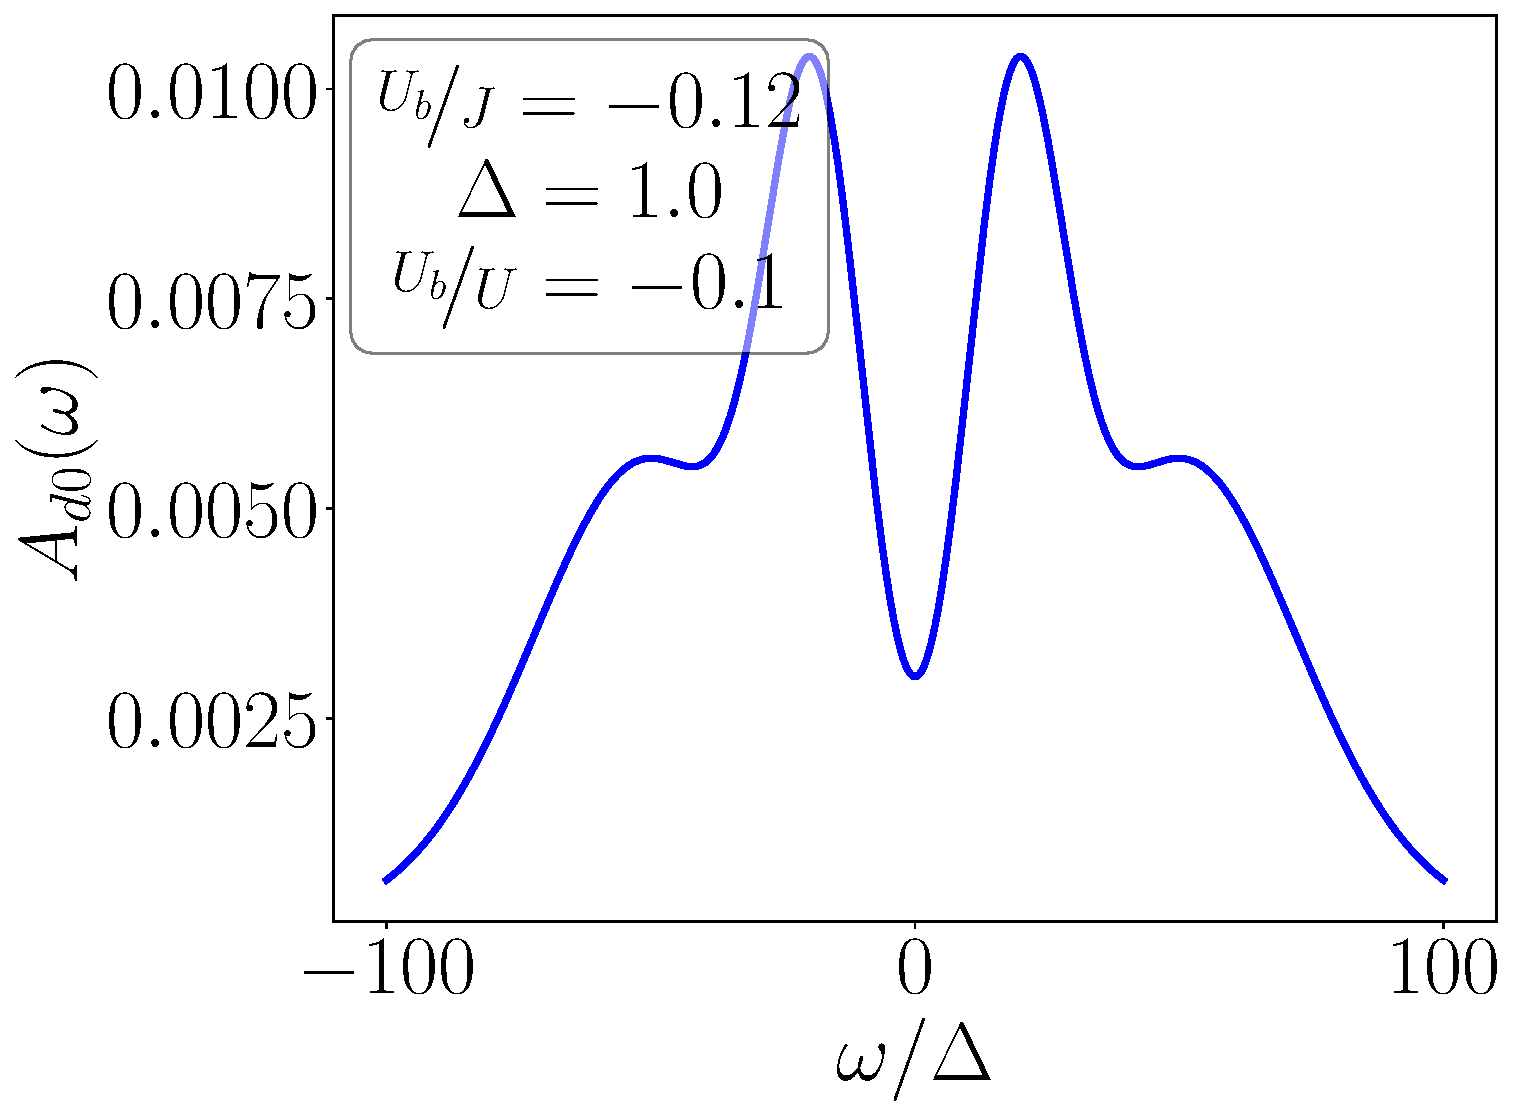
\includegraphics[width=0.33\textwidth]{./figures/spec_func_00_Ub_by_J=-0.125.pdf}
\hspace*{\fill}

\hspace*{\fill}
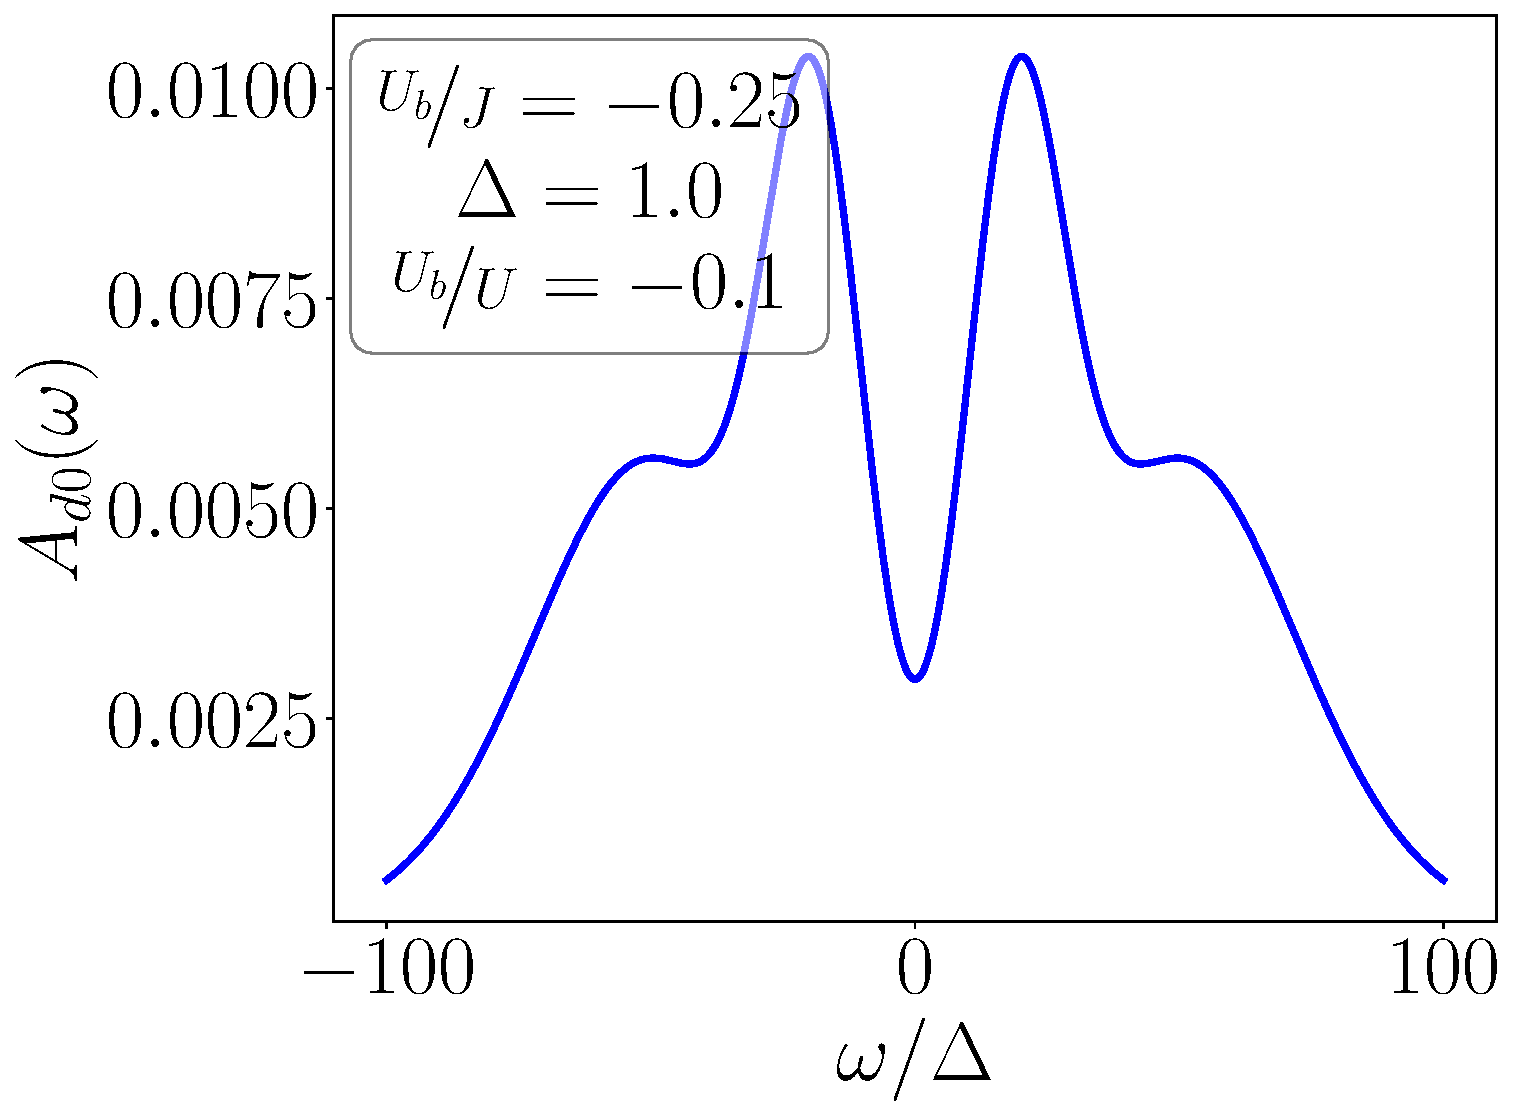
\includegraphics[width=0.33\textwidth]{./figures/spec_func_00_Ub_by_J=-0.250.pdf}
\hspace*{\fill}
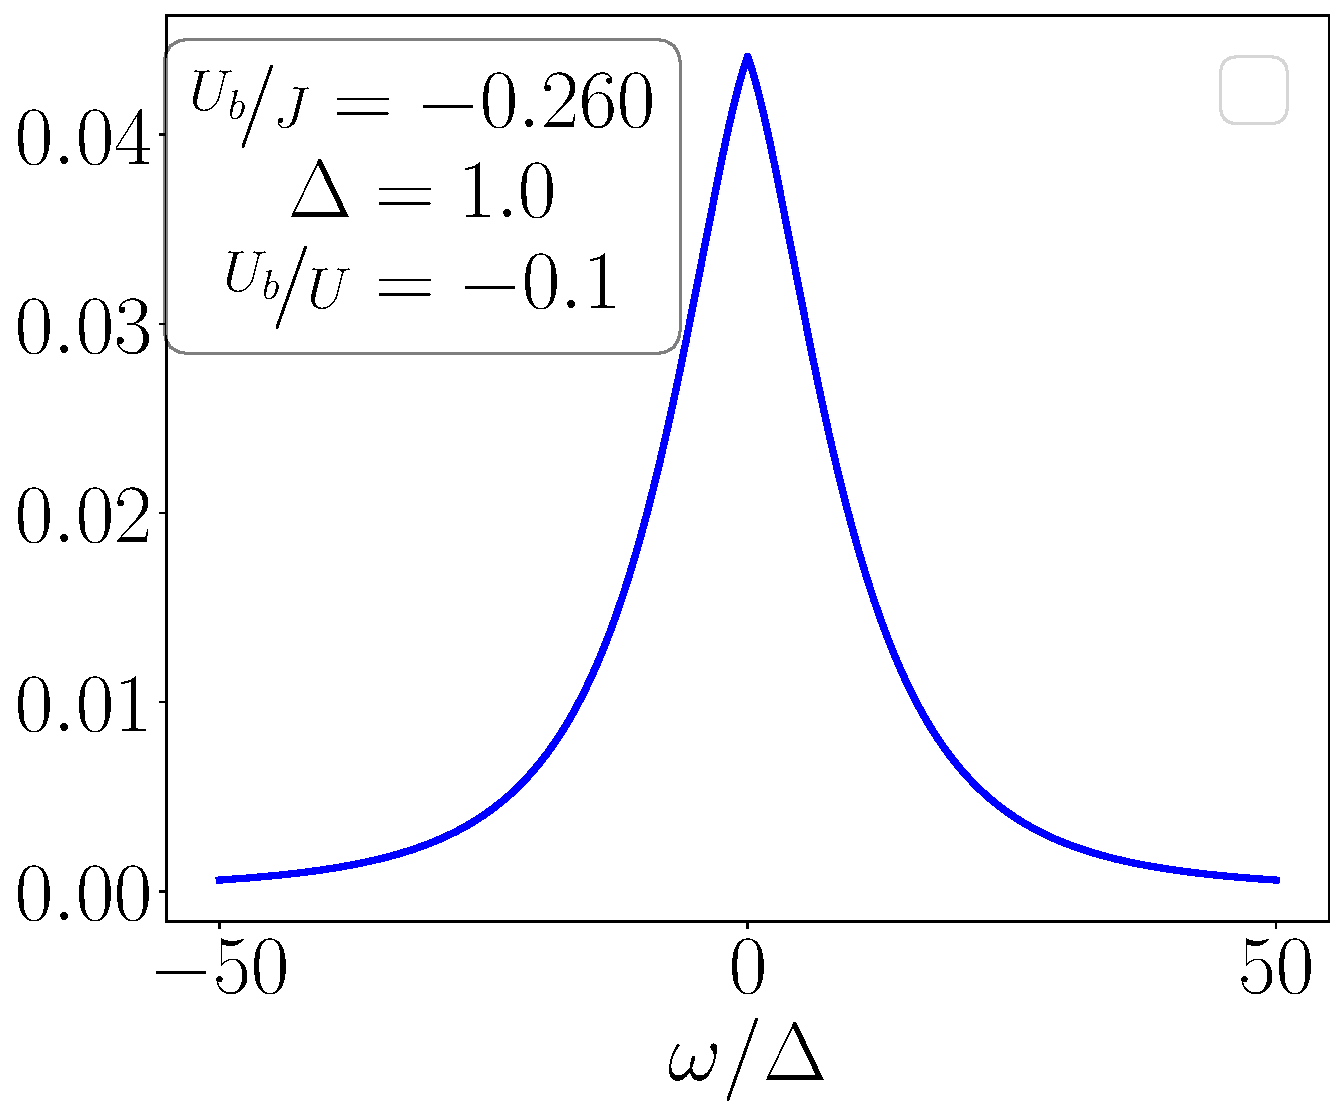
\includegraphics[width=0.29\textwidth]{./figures/spec_func_00_Ub_by_J=-0.26.pdf}
\hspace*{\fill}
\end{frame}

\section{The Auxiliary Model Approach}
\label{aux-method}

\begin{frame}[noframenumbering]{General philosophy}
\vspace*{-20pt}
	\[H = \overbrace{H_\text{cluster}}^\text{simple} + \underbrace{H_\text{bath} + H_\text{cl-bath}}_\text{complicated}\]
\begin{itemize}
	\item find "appropriate" bath and then solve the cluster+bath problem
	\item appropriate = physical + solvable
\end{itemize}

\centering
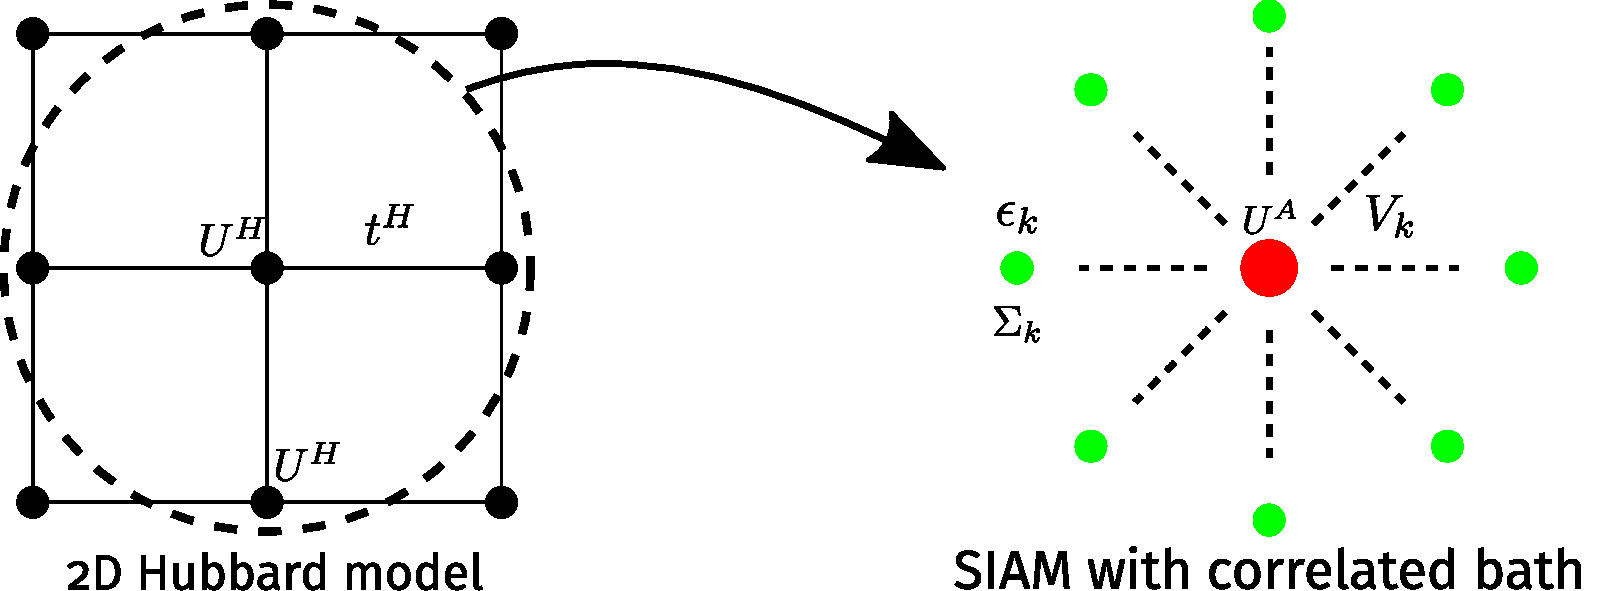
\includegraphics[width=0.8\textwidth]{./figures/cluster-bath.pdf}
\end{frame}

\begin{frame}[noframenumbering]{The present method}
\centering
\begin{itemize}[<+->]
\item \focus{Choose an auxiliary model} \(H_\text{aux}\) consisting of a correlated impurity interacting with a minimally correlated bath
\item \focus{Solve} this impurity model \(H_\text{aux}\) using the unitary RG
\item Create a \focus{bulk lattice model} \(H_\text{bulk}\) from this auxiliary model \(H_\text{aux}\) by applying translation operators on the latter
\item The relation hence obtained between the impurity and bulk models then allows us to \focus{relate the physics} of the two.
\end{itemize}

\only<1>{
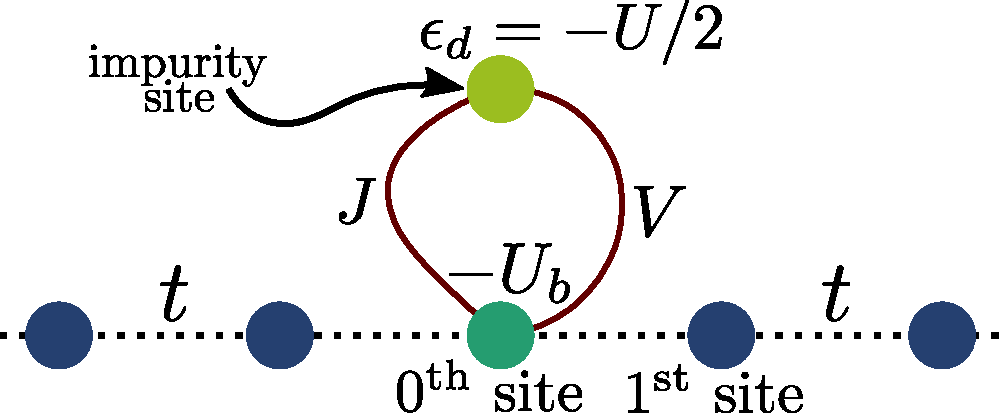
\includegraphics[height=0.4\textheight]{./figures/gen_siam.pdf}}
\end{frame}

\section{The Tiling Process}
\label{tiling}

\begin{frame}[noframenumbering]{Creating the unit of tiling}
\begin{itemize}[<+->]
\item Replace impurity index with one particular lattice site \(i\)
\item Replace bath with the remaining \(N-1\) sites of lattice
\item Replace the zeroth site with one of the neighbours \(j\) of \(i\)
\end{itemize}
\only<3>{
\centering
\[\mathcal{H}_\text{aux}(i,j) = \text{KE}_\text{rem.} - \frac{U}{2}\left( \hat n_{i \uparrow} - \hat n_{i \downarrow} \right) ^2 + V \sum_{\sigma} \left(c^\dagger_{j\sigma} c_{i\sigma} + h.c.\right) +J \vec{S_i}\cdot\vec{S}_j - U_b\left(\hat n_{j \uparrow} - \hat n_{j \downarrow}\right)^2\]
\includegraphics[height=0.4\textheight]{./figures/tiling_small.pdf}
}
\end{frame}

\begin{frame}[noframenumbering]{Creating the bulk model}
\begin{itemize}[<+->]
	\item Average over all \(w\) nearest neighbours
		\[\mathcal{H}_\text{aux}(i) = \frac{1}{w}\sum_j \mathcal{H}_\text{aux}(i,j)\]
	\item Translate over all lattice sites \(i\)
		\[\mathcal{H}_\text{full} = \sum_i \mathcal{H}_\text{aux}(i)\]
\end{itemize}
\vspace*{-10pt}
\only<2>{\centering
\includegraphics[height=0.35\textheight]{./figures/tiling_all.pdf}}
\end{frame}

\begin{frame}[noframenumbering]{Result of tiling}
We end up with a \focus{Hubbard-Heisenberg} model.
\[\mathcal{H}_{H-H} = -\sum_{i} U_H \left(\hat n_{i \uparrow} - \hat n_{i \downarrow} \right)^2 - t_H\sum_{<i,j>,\sigma}\left(c^\dagger_{i\sigma}c_{j\sigma} + \text{h.c.}\right) + J_H\sum_{<i,j>} \vec{S}_i\cdot\vec{S}_j\]

The mapping between the parameters is
\[t_{H-H} = \left(2t (N-2) - \frac{2V}{N}\right),~ ~ U_{H-H} = \left(\frac{U}{2} + U_b\right), ~ ~ J_{H-H} = \frac{2J}{w}\]
\end{frame}

\section{Greens functions, spectral functions and self-energy}
\label{greens}

\begin{frame}[noframenumbering]{Strategy}
	\begin{itemize}
	\item Replace the Hamiltonian for inverse Greens operators
	\item Use equation to relate bulk and impurity inverse Greens operators
	\item Use spectral representation to invert them and obtain Greens functions
	\item Use Greens functions to compute the rest
	\end{itemize}
\end{frame}

\begin{frame}[noframenumbering]{Inverse Greens operator}
Define inverse Greens operators:
\[\mathcal{G}_\text{aux}(i) = \frac{1}{\omega - \left(H_\text{aux}(i) - E_\text{gs}\right)}\]
\[\mathcal{G}_{H-H} = \frac{1}{N \omega - \left(H_{H-H} - N E_\text{gs}\right) }\]
Replace in tiling expression:
\[\mathcal{G}^{-1}_{H-H} = \sum_i \mathcal{G}^{-1}_\text{aux}(i) = \frac{1}{w}\sum_{i, j \in \text{NN of i}}\mathcal{G}^{-1}_\text{aux}(i,j)\]
\end{frame}

\begin{frame}[noframenumbering]{Matrix elements of \(\mathcal{G}_\text{H-H}^{-1}\)}
Particle excitation on ground state of auxiliary model:
\[\ket{i} \equiv c^\dagger_{i\sigma}\ket{\Phi_0}\]
\only<+>{
	\focus{Local} matrix elements \(\left(\mathcal{G}^{-1}_{H-H}\right)^p_{ii}\) depend on the auxiliary model at \(i\):
\[\left(\mathcal{G}^{-1}_{H-H}\right)^p_{ii} = \underbrace{w\times \frac{1}{w} \braket{\Phi_0 | c_{i\sigma} \mathcal{G}^{-1}_\text{aux}(i) c^\dagger_{i\sigma} | \Phi_0}}_\text{\(w\) nearest neighbour pairs} = \braket{\Phi_0 | c_{d\sigma} \mathcal{G}^{-1}_\text{aux}(d) c^\dagger_{d\sigma} | \Phi_0}\]
\centering
\includegraphics[width=0.4\textheight]{./figures/Gf_nlocal.pdf}
}
\only<+>{
	\focus{N-neighbour} elements \(\left(\mathcal{G}^{-1}_{H-H}\right)^p_{i,i+1}\) depend on the aux. model at \(i\) with \(0^\text{th}\) site at \(i+1\):
	\[\left(\mathcal{G}^{-1}_{H-H}\right)^p_{i,i+1} = \underbrace{\frac{1}{w}\braket{\Phi_0 | c_{d\sigma} \mathcal{G}^{-1}_\text{aux}(d) c^\dagger_{z,\sigma} | \Phi_0}}_\text{one nearest-neighbour pair}\]
\centering
\includegraphics[width=0.4\textheight]{./figures/Gf_local.pdf}
}
\end{frame}

\begin{frame}[noframenumbering]{Spectral representation of \(\mathcal{G}_\text{H-H}^{-1}\) in eigenstates of \(\mathcal{H}_\text{aux}\)}
Eigenstates of \(\mathcal{H}_\text{aux}: \ket{\Phi_n}\)

\only<+>{
Insert \(1 = \sum_m \ket{m}\bra{m}\):
\[\left(\mathcal{G}^{-1}_{H-H}(\omega)\right)^p_{ii} = \sum_{m} |d^p_m|^2 \left(\mathcal{G}^{-1}_\text{aux}(d, \omega)\right)_{mm}\]
where \(d_m^p\) is the spectral weight factor:
\[d^p_m = \bra{\Phi_m}c^\dagger_{d\sigma}\ket{\Phi_0}\]
}
\only<+>{
	Similarly, the off-diagonal matrix element also has a spectral representation:
	\[\left(\mathcal{G}^{-1}_{H-H}\left(\omega\right) \right)^p_{i,i+1} = \frac{1}{w} \sum_n \left(d^p_m\right)^* z^p_m \left(\mathcal{G}^{-1}_\text{aux}(d, \omega) \right)_{mm}\]
where
\[z_m^p = \braket{\Phi_m | c^\dagger_{z\sigma} | \Phi_0}\]
}
\end{frame}

\begin{frame}[noframenumbering]{Hole counterparts}
	\begin{itemize}
		\item Hole excitations can be similarly obtained by considering states \(\ket{\tilde i} = c_{i\sigma}\ket{\Phi_0}\)
		\item Identical process but replace spectral weight factors with hole counterparts:
			\[d^p_m = \bra{\Phi_m}c^\dagger_{d\sigma}\ket{\Phi_0} \to d^h_m = \bra{\Phi_m}c_{d\sigma}\ket{\Phi_0}\]
	\end{itemize} 
The corresponding relations are
\[\left(\mathcal{G}^{-1}_{H-H}(-\omega)\right)^h_{ii} = \sum_{n} |d^h_n|^2 \left(\mathcal{G}^{-1}_\text{aux}(d, -\omega)\right)_{nn}\]
\[\left(\mathcal{G}^{-1}_{H-H}\left(-\omega\right) \right)^h_{i,i+1} = \frac{1}{w} \sum_n \left(d^h_n\right)^* z^h_n \left(\mathcal{G}^{-1}_\text{aux}(d, -\omega) \right)_{nn}\]
\end{frame}

\begin{frame}[noframenumbering]{Summary}
	\begin{itemize}
	\item We have expressed matrix elements of the bulk in terms of those of the auxiliary model
	\item The spectral representation allows the right-hand side to have only diagonal matrix elements
	\item This makes it easier to invert them
	\end{itemize}
\end{frame}

\begin{frame}[noframenumbering]{Inversion and single-particle Greens functions}
	Since \(\mathcal{G}^{-1}_\text{aux}(d, -\omega)\) is diagonal in the basis of \(\ket{\Phi_n}\), we can simply write
	\[\left(\mathcal{G}^{-1}_{H-H}(\omega)\right)^p_{ii} = \sum_{m} |d^p_m|^2 \left(\mathcal{G}^{-1}_\text{aux}(d, \omega)\right)_{mm} \implies \left(\mathcal{G}_{H-H}(\omega)\right)^p_{ii} = \sum_{n} |d^p_n|^2 \left(\mathcal{G}_\text{aux}(d, \omega)\right)_{nn}\]
The Greens function can be related to the Greens operator:
\[G({i}, j, \omega) = \bra{{i}} \mathcal{G}(\omega, H) \ket{j} - \bra{\tilde{j}} \mathcal{G}(-\omega, H) \ket{\tilde{i}}\]
Using this, we can finally write down the Greens functions:
\[\left(G_{H-H}(\omega)\right)_\text{loc} = \sum_n \left[|d^p_n|^2 \left(\mathcal{G}_\text{aux}(d, \omega)\right)_{nn} - |d^h_n|^2 \left(\mathcal{G}_\text{aux}(d, -\omega)\right)_{nn}\right]\]
\[\left(G_{H-H}(\omega)\right)_\text{n-n} = \frac{1}{w}\sum_n \left[\left(d^p_n\right)^* z^p_n \left(\mathcal{G}_\text{aux}(d, \omega) \right)_{nn} - \left(z^h_n\right)^* d^h_n \left(\mathcal{G}_\text{aux}(d, -\omega)\right)_{nn}\right]\]
\end{frame}

\begin{frame}[noframenumbering]{\(k-\)space Greens function, spectral function and self-energy}
The \(k-\)space Greens function will be approximated by the local and nearest-neighbour Greens functions:
\[G_{H-H} (\vec k, \omega) \simeq G_{H-H} (\omega)_\text{loc} + G_{H-H} (\omega)_\text{n-n}\sum_{i=1}^w e^{i \vec{k}\cdot\vec {a_i}} = G_\text{aux}(dd, \omega) + \frac{\xi_{\vec k}}{w}G_\text{aux}(d0, \omega)\]
Taking the imaginary part gives the \focus{spectral function}:
\[A_{H-H} (\vec k, \omega) = A_\text{aux}(dd, \omega) + \frac{\xi_{\vec k}}{w}A_\text{aux}(d0, \omega), ~ ~ ~ \xi_{\vec k} = \sum_{i=1}^w e^{i \vec{k}\cdot\vec{a}_i}\]
From Dyson's equation, we get \focus{self-energy}:
\[\Sigma(\vec k, \omega) = G_0(\vec k, \omega)^{-1} - G(\vec k, \omega)^{-1} = \omega +t^{H-H}\xi_{\vec k} - \left [G_\text{aux}\left(dd, \omega\right) + \frac{\xi_{\vec k}}{w} G_\text{aux}\left(d0, \omega\right)\right]^{-1}\]
\end{frame}

\section{Evidence for the Mott MIT}
\label{mit}

\begin{frame}[noframenumbering]{Evidence for Mott MIT}
\begin{itemize}[<+->]
	\item \focus{one-to-one mapping} between Greens functions of the bulk and the auxiliary models
	\item low energy resonance in the impurity excitations implies \focus{propagation} of $e^{-}$s across lattice
	\item gap in the impurity excitations implies $e^{-}$s are "stuck" and \focus{spectral flow is not possible}
	\item Constraining \(U_b\) to, say, \(-U/10\), we get a critical ratio:
		\[\frac{U_\text{H-H}^*}{J^*_\text{H-H}} = \frac{w}{4}\left(\frac{U^*}{J^*} - \frac{1}{2}\right) = 2\]
		where we used \(w=4\) for a  2D square lattice.
\end{itemize}
\vspace*{-40pt}
\only<1>{
\centering
\includegraphics[height=0.24\textwidth]{./figures/spec_func_Ub_by_J=-0.100.pdf}
\includegraphics[height=0.24\textwidth]{./figures/spec_func_Ub_by_J=-0.250.pdf}
\includegraphics[height=0.24\textwidth]{./figures/spec_func_Ub_by_J=-0.26.pdf}
}
\only<2>{
\centering
\includegraphics[height=0.25\textheight]{./figures/metal_prop.pdf}
}
\only<3>{
\centering
\includegraphics[height=0.25\textheight]{./figures/ins_prop.pdf}
}
\end{frame}

\section{Final Remarks}
\label{concl}

\begin{frame}[noframenumbering]{Conclusions}
	\begin{itemize}[<+->]
		\item The auxiliary model method described here provides a \focus{constructionist} approach to studying systems of strong correlations
		\item \focus{Minimal attractive interaction} on bath leads to a metal-insulator transition in the Hubbard-Heisenberg model
		\item The transition derives from a competition between \focus{Kondo} spin-flip physics and the physics of \focus{pairing} instability.
\end{itemize}
\end{frame}

\begin{frame}[noframenumbering]{Moving forward}
\begin{itemize}[<+->]
	\item \(k-\)dependence of the self-energy: \focus{electronic differentiation} and effects of Van Hove singularities?
	\item Breaking particle-hole symmetry on the impurity will allow us to study bulk models \focus{away from half-filling}.
	\item For more accurate results, one can consider \focus{multiple impurities} in the cluster.
\end{itemize}
\only<3>{\centering\includegraphics[height=0.3\textheight]{./figures/dimer_dispersion.pdf}}
\end{frame}

\section{Thank you.}


\end{document}
